\documentclass[a4paper]{article}
\usepackage[utf8]{inputenc}
\usepackage{float}
\usepackage{pdfpages}
\usepackage{textcomp}
\usepackage{indentfirst}

\setlength{\parskip}{1em}

% Colour Management
\usepackage{color}

% Multi-Line Com ments
\usepackage{comment}

% Customisable Sections
\usepackage{titlesec}
\titleformat{\paragraph}[hang]{\normalfont\normalsize\bfseries}{\theparagraph}{1em}{}
\titlespacing*{\paragraph}{0pt}{3.25ex plus 1ex minus .2ex}{1em}

% Images and Captions
\usepackage{graphicx}
\usepackage{subcaption}
\usepackage{wrapfig}
\graphicspath{{./images/}}
\usepackage{fancyhdr} 


% Bibliography
\usepackage[nottoc]{tocbibind}
\usepackage[
    backend=biber,
    sorting = none, 
    style=ieee]{biblatex}

\addbibresource{report_citations.bib} %Imports bibliography file

\usepackage{amsmath} %sudo tlmgr install amsmath


% Tables
\usepackage{array}
\newcolumntype{L}{>{\raggedright\arraybackslash}m{0.9\linewidth}}
\usepackage{ragged2e}
\usepackage{hhline}
\usepackage{multicol}
\usepackage[outdir=./media]{epstopdf}

% Contents Page
\usepackage{hyperref}

% Appendices
\usepackage[toc,page]{appendix}

% Bold Maths Symbols
\usepackage{bm}
\usepackage{gensymb} %sudo tlmgr install was
\usepackage{multicol}

%Command for adding units to equations
\newcommand{\unit}[1]{\ensuremath{\, \mathrm{#1}}}


% Allowing lower levels of Contents Page
\setcounter{tocdepth}{4}
\setcounter{secnumdepth}{5}

% Make margins smaller, feel free to change
\usepackage{geometry}
\geometry{
    a4paper,
    top = 20mm,
    bottom = 20mm,
    textwidth=450pt
}





\title{Engineering Design Project}
\author{Georgios Chaimalas \and 
        Dimitrios Georgakopoulos \and 
        Edvard J. Skaarberg Holen \and 
        Hyunjoon Jeon \and 
        Josiah Mendes \and 
        Raghav Viswakumar}
\begin{document} 
\begin{titlepage}
    \setlength{\headheight}{66.89pt}
    \thispagestyle{fancy}
    \renewcommand{\headrulewidth}{0pt}
    \renewcommand{\footrulewidth}{0pt}
    \lhead{
\includegraphics[scale=0.1]{logo.png}}
    \cfoot{} % this is to remove the page number
    \hbox{}\vfill
    \begin{center} 
	    {\scshape\LARGE Imperial College London  \par}
	    \vspace{1cm}
        {\scshape\Large Second Year Design Project\par}
        \vspace{0.25cm}
        {\scshape\Large ELEC50003/ELEC50008\par}
        \vspace{1.5cm}
        {\huge\bfseries The MARS Rover\par}
        \vspace{2cm}
        {\Large\itshape Group 1\par}
        \vfill
        \begin{flushright}
            \textsl{ \large
            Georgios Chaimali \\ 
            Dimitrios Georgakopoulos \\ 
            Edvard J. Skaarberg Holen \\ 
            Hyunjoon Jeon \\ 
            Josiah Mendes \\ 
            Raghav Viswakumar
            }
        \end{flushright}
        \vfill

        % Bottom of the page
        {\large Word Count: XXXX Words \\ \today\par}
        \vfill
    \end{center}
\end{titlepage}
 
\setcounter{tocdepth}{2}
\tableofcontents

\newpage

\section{Introduction}

The aim of the Mars Rover Project as outlined by our organisers is as 
follows: “to design and build an autonomous rover system that could be 
used in a remote location without direct  supervision”\cite{MarsRoverSpec}.  
To fulfil this broad goal, the design and development of the rover is separated into 
six distinct subsystems: \textbf{Command, Control, Drive, Energy, Integration and Vision},
each of which will be led by a single team member. These modules will work semi-independently to 
achieve the functional requirements as defined by the problem and 
eventually integrate their findings and goals to achieve the goals set out by the specification 
at hand. We will work under the main consideration that our rover is meant 
to be a proof of concept for one that could function on Mars. This report 
contains our design process for the rover, how it was implemented and challenges that were faced. 

\section{Structural Design }

\begin{figure}[H]
	\begin{Center}
		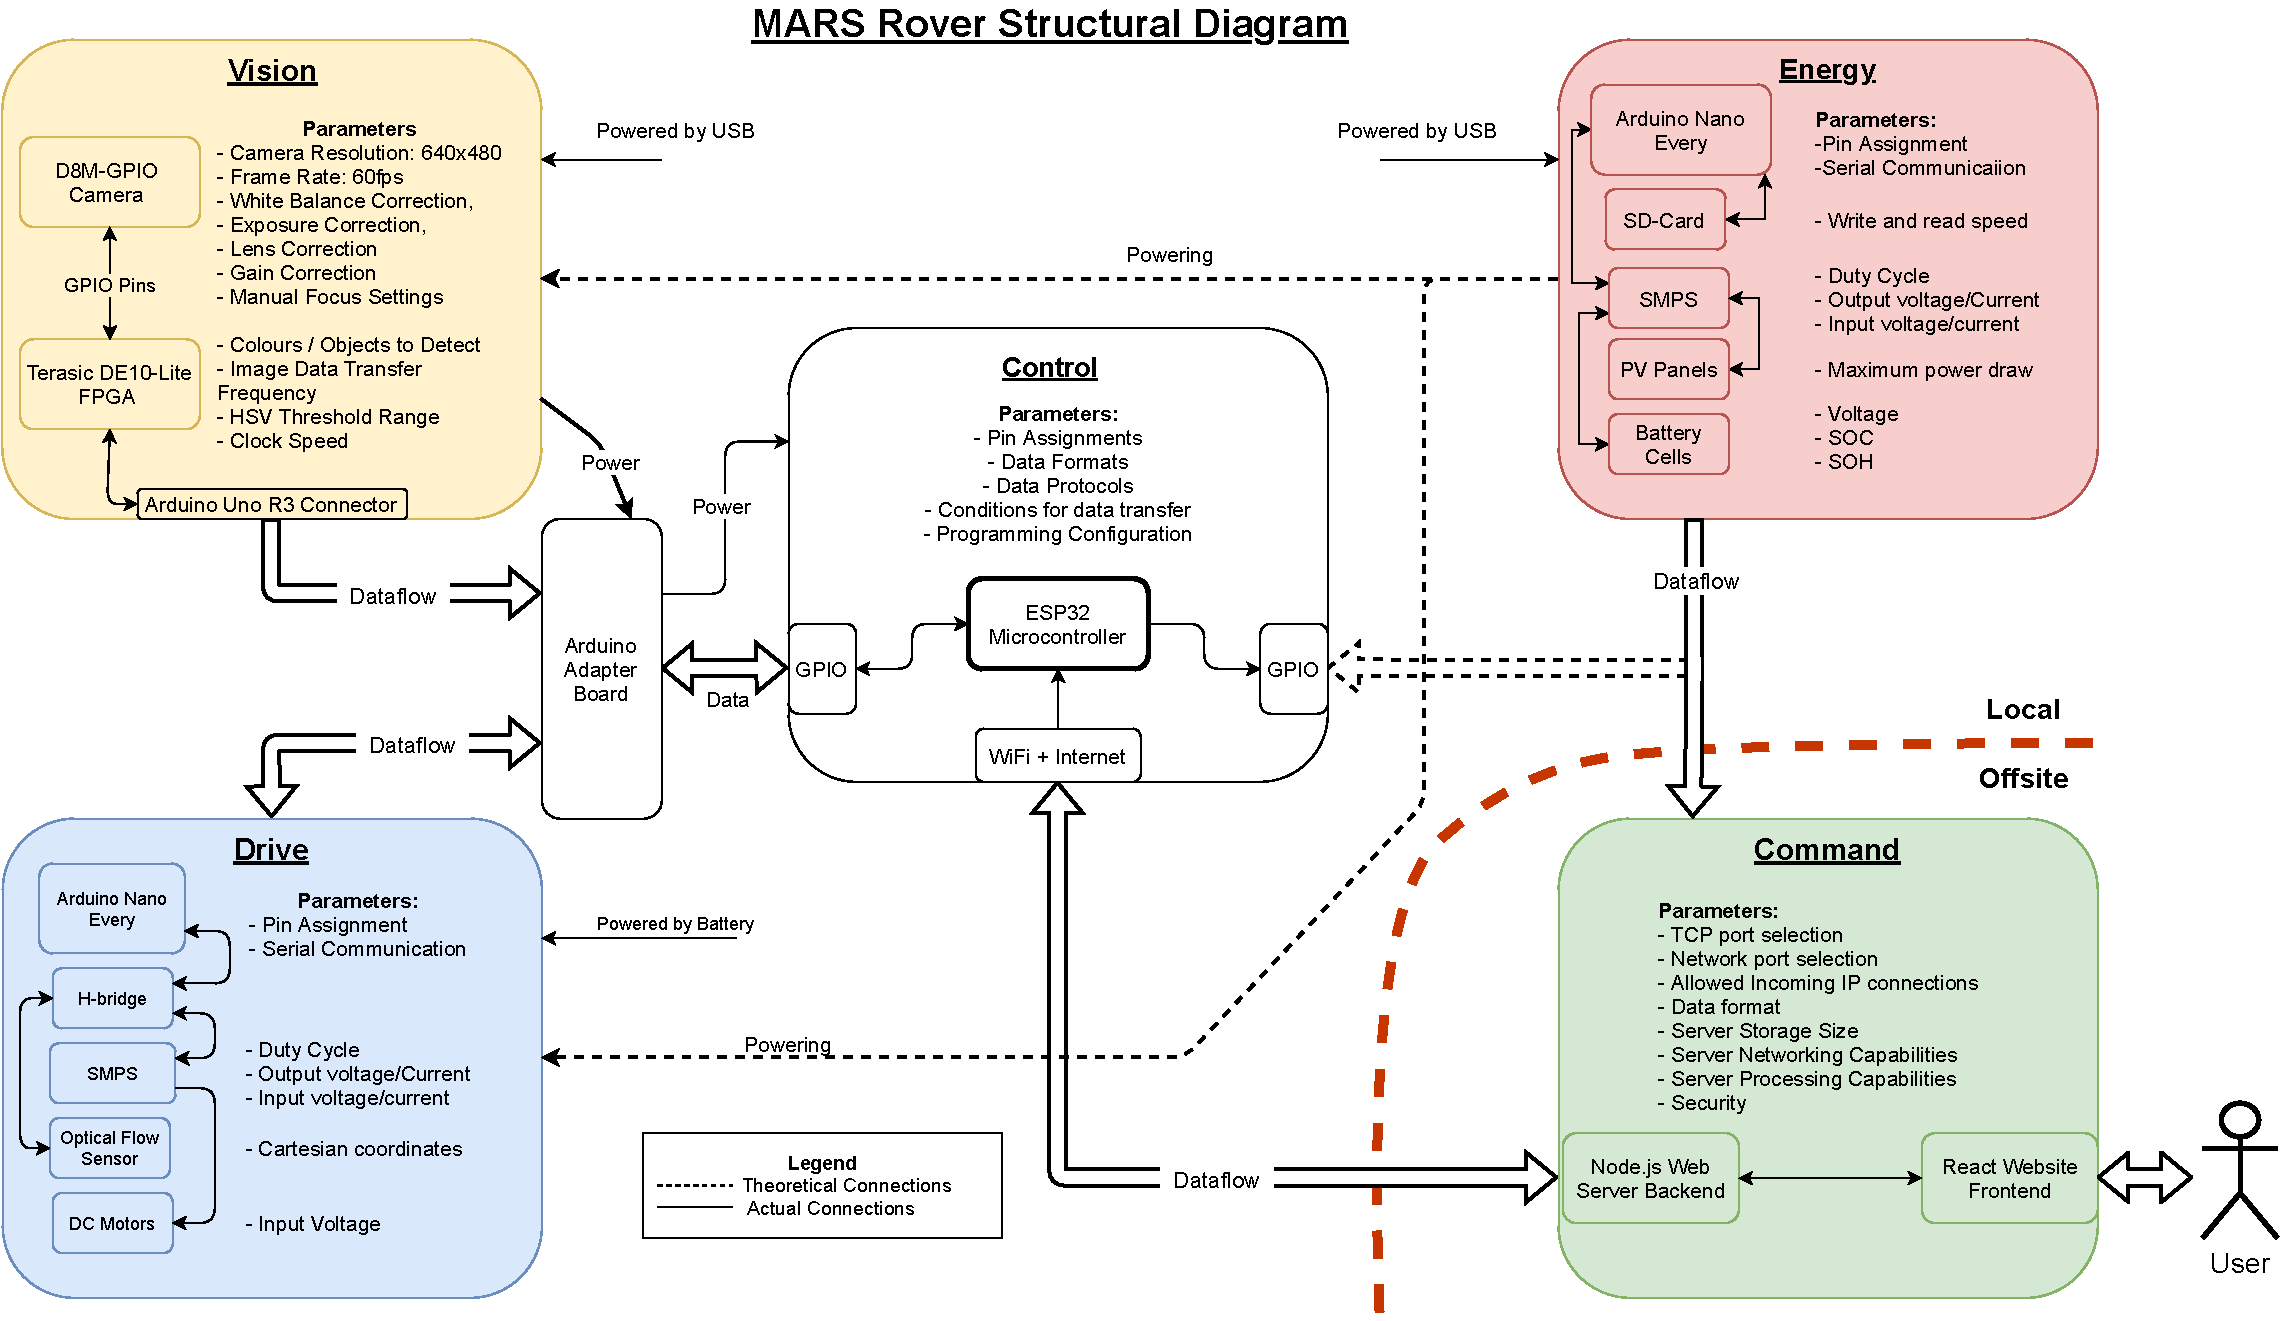
\includegraphics[width = \linewidth]{./media/StructuralDiagram.pdf}
		\caption[Structural Design Diagram showing Hardware and Parameters of Subsystems for Mars Rover]{\protect\raggedright Structural Design Diagram showing Hardware and Parameters of Subsystems for Mars Rover}
		
        \label{fig:StructuralDesignDiagram}
	\end{Center}
\end{figure}

The structural design of the Rover as shown in Figure \ref{fig:StructuralDesignDiagram}, shows
the 5 main subsystems of the rover together with their main hardware components. 
This presents an overview of the entire Rover system and how the different components 
interact with each other. Both power connections and data connections are shown, 
together with corresponding arrows where directional transfer is necessary. 
Each subsystem's hardware has a set of configurable parameters that are also shown,
these parameters are determined as part of the functional design process and 
implementation.  

\section{Functional Design}

\subsection{Control}

\begin{figure}[H]
	\begin{Center}
		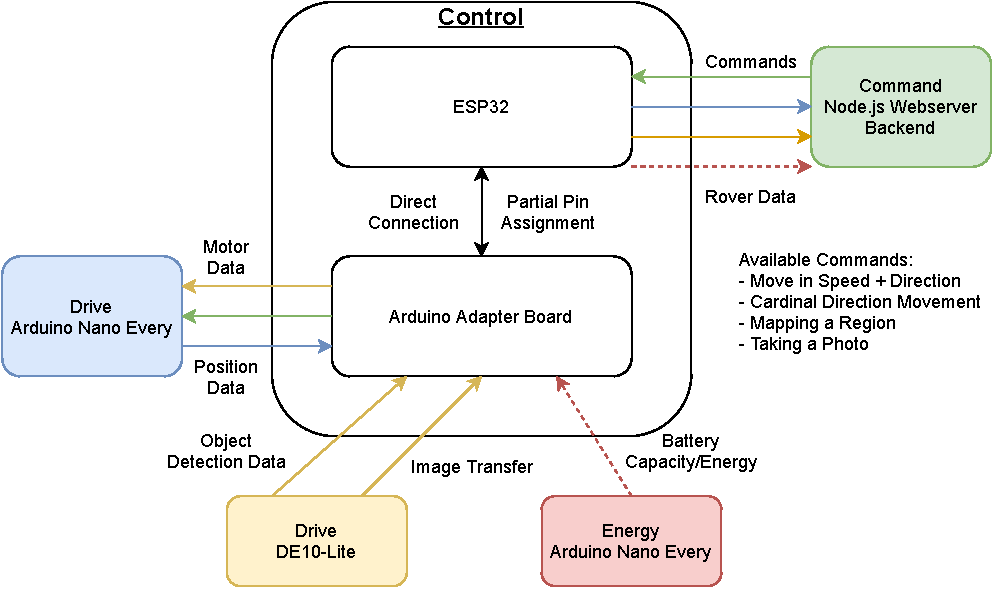
\includegraphics[width = \linewidth]{./media/ControlFunctional.pdf}
		\caption[Functional Design Diagram showing Dataflow for Control Subsystem]{\protect\raggedright Functional Design Diagram showing Dataflow for Control Subsystem}
        \label{fig:ControlFunctionalDiagram}
	\end{Center}
\end{figure}

\subsubsection{Requirements}

The Control module within the context of the rover has one main goal: 
\textbf{to act as the communication hub between all the subsystems, delivering
the relevant data where it is required to allow for the rover to integrate
as a whole} \cite{MarsRoverSpec}.  These functional requirements can be 
obtained from the Functional Design diagram for control, see Figure \ref{fig:ControlFunctional}, outlining all the 
data flow for the Control subsystem. There are a couple of core objectives 
which must be achieved in order to fulfil this role as outlined below:

\begin{enumerate}
    \item Act as a WiFi Access Point sitting under a router to receive
    commands from the Command subsystem and send data through 
    socket-level communication.
    \item Use a relevant hardware-level data transmission protocol to
    send movement commands to the Drive subsystem and receive data for 
    Command. 
    \item Use a relevant hardware-level data transmission protocol to 
    receive the Vision subsystem data.
    \item Connect the Energy subsystem with the rover, sending the 
    relevant data to the Command subsystem.
\end{enumerate}

Although the hardware is fixed, the solutions to the outlined problems
above are mostly up to design. It is for this reason that the main 
challenge stems from understanding what works best for communication 
to each subsystem and more importantly, how to integrate it such that 
the transmission of data can be smoothly facilitated through the ESP32.

\subsubsection{Hardware Organisation}

The Control module comprises of two hardware components \cite{BoxContent}: 
the ESP32, a system on chip microcontroller \cite{ESP32Datasheet}, as 
well as an Arduino adapter board designed to map some of the available 
GPIO pins on the ESP32 to an Arduino-like board \cite{ESP32ArduinoAdapter}.

This hardware was provided by the project organisers and it immediately 
limits the tools which can be used, however the wide array of functionality 
which this microcontroller can provide through programming the chip allows
for sufficient freedom and capabilities to complete the required tasks. The
GPIO pins are highly configurable when compared to an Arduino-Uno 
\cite{MicrocontrollerComparison}, as they are capable of using more data 
communication through almost any of the pins via software configuration 
\cite{ESP32PinOut}. It is low-cost and low-power, capable of using 
WiFi capabilities at 2.4GHz and Bluetooth \cite{ESP32Datasheet} to 
interface wirelessly with other devices. Using the Arduino Adapter 
board \cite{ESP32ArduinoAdapter}, it can sit directly on top of an 
Arduino or device with similar pins to directly interface through 
physical connections like the FPGA in this case. 

For wired communications, the ESP32 has limitations for the type of 
communication peripherals it can use with peer microcontrollers. 
Unlike Arduinos which have at most 1 SPI, 2 I2C and 1 UART port 
\cite{ArduinoPeripheral}, the ESP32 can support up to 3 SPI, 2 I2C and 
3 UART ports \cite{ESP32Datasheet} which are configurable to most of 
the GPIO pins available. Considering the ESP32 will have to interface with 
at most three other subsystems through wired communication, 
there is a lot of choice with peripherals that must be evaluated.

As the three most common hardware peripherals to use in any engineering
project, there is a discussion to be had about the differences between
UART, SPI and I2C \cite{CommProtocolComp}. UART and I2C utilise 2 ports 
for connections on eachdevice while SPI uses 4. While UART and SPI 
are full-duplex, allowing for simultaneous data transfer between devices, 
this is not the case for I2C. With regards to complexity, UART is the 
simplest form of transfer that is available. Due to the number of 
devices in SPI and I2C able to exceed 2, in comparison to UART, they 
can be much harder to set up as they include additional checks to reflect
their multiple device support. While I2C and SPI may be faster methods for 
data transfer, they limit flexibility in design as I2C for example, 
requires one device to designate itself as a controller and another as a 
peripheral, which is not ideal for devices which need to regularly 
instantiate communication with one another as controllers.

\subsubsection{Initial Design Choices} 

There are many options available for programming the ESP32. Due to the 
lax requirements with regards to communication, it was quickly determined 
that the Arduino IDE and supporting libraries for the ESP32 would be 
enough for developing what is necessary. As there are stringent practices 
for the base Arduino Libraries and ESP8266 Libraries, this was extended 
to a majority of the functionality available to the ESP32 including WiFi, 
Bluetooth, UART, SPI and I2C \cite{ESP32ArduinoGithub}. Seeing as the ESP32 
through Espressif is programmed through C, most of this can be imported 
through the Arduino IDE which supports simpler methods for flashing 
software onto the ESP32.

As there is no requirement imposed upon the data being transferred 
and displayed, this results in complete freedom for the form in which 
data is communicated through the ESP32 and whether it should be processed. 
Seeing as the ESP32 will be handling communication between four other 
subsystems, it was decided that the amount of processing on the device 
should be limited as much as possible and offloaded to the other 
subsystems. This is to ensure that bottlenecks would not appear due to a 
sizable processing time in between transmission of data, as this would 
cause crippling delays for communication. The simplest way to ensure the 
integrity of the data is to standardise the type for data being 
transferred. Since initially, the formatting and content of the data was 
unclear, receiving and sending them as bytes or characters would be the 
most versatile solution. Internal buffers for the ESP32 would store 
individual commands or data lines and send them to the required subsystem 
for processing.

With regards to the communication between Command and Control, 
there were a couple of options available. As the Command subsystem 
would be hosted on a website, we could choose from application layer 
protocols like HTTPs or MQTT, but as we decided our application was 
more simplistic with regards to the type of data being communicated, we 
opted for the transport layer protocol, TCP. This is due to the need for 
consistent transmission of data, retransmitting if packets are lost and 
ensuring the data does reach its destination. Speed by comparison is a 
less stringent requirement and as such, UDP was discarded as a choice
\cite{TCPvsUDP}.

For both Drive and Energy, the Arduino Nano Everything provided by the 
project organisers had it’s UART ports exposed through the specific 
hardware and it’s connections. As such, there was little need for 
deliberation over the protocol being used \cite{ArduinoSerial}. The 
peripheral chosen for both these groups was UART. For the Energy 
submodule specifically, since it can’t be integrated into the Rover 
physically, it was decided that any necessary data would be transmitted 
directly to Command. This is through the UART USB connection from the 
Arduino to the computer, which would then communicate with Command over 
TCP. However, to ensure Energy can be integrated if necessary, one UART 
port for the ESP32 was set aside for Energy.

For Vision, there are two types of data which need to be transferred 
through the ESP32; the image from the camera and data regarding object 
detection which could include values like distance to the object. Since 
the image transfer will likely take a long time to accomplish, a decision
was made to dedicate two peripherals between Vision and Control. 
Considering the ESP32 will sit on top of the DE10-Lite FPGA, the 
availability of ports is not a concern. As two UART ports are unavailable 
since one will be used to communicate with Drive and the other is 
dedicated for Energy, the peripherals chosen instead will be SPI. 
One SPI connection is dedicated to sending images while the other is 
dedicated to sending any data between the ESP32 and the FPGA.

\subsection{Command}

\subsubsection{Requirements}

The Command module has three main purposes within the system of the rover:

\begin{enumerate}
    \item Visualise data from the other subsystems
    \item Allow users to command the rover
    \item Calculate paths for the rover to follow based on the commands given by the users
\end{enumerate}

In order to achieve the aforementioned goals, it was important to establish 
connection between the Command module as a server, and other subsystems as 
clients. The ESP32 of the Control module is the main client that constantly 
communicates with the server to exchange commands and status of the rover. 
The energy module is another client and regularly sends data related to the 
battery of the rover. The received data are presented on a web application 
where users can check the current status of the rover and command the rover. 
In order to smoothly handle incoming data and render components that form the 
web application, the web application was divided into the server-side: backend, 
and the presentation side: frontend, written in Node js and React respectively.

\subsubsection{Hardware Organisation}

Unlike the other subsystems of the rover, the Command module does not require any 
hardware components except a laptop on which the web application would be running. 
Therefore, the main focus was put on choices of tools for building the web application 
and communication methods between the other submodules and the backend, and between the 
backend and the frontend of the web application. 

\subsubsection{Initial Design Choices}

For building a website, the Hypertext Markup Language (HTML) and Cascading Style Sheets (CSS) would 
be used. The two technologies are chosen because the HTML allows programmers to describe the structure 
of the website in the form of document while CSS offers tools to style the individual components of 
the website. With CSS, it would also be possible to create graphics which may visualise data in a more 
sophisticated way. React js, the language in which the frontend of the website is written, allows rendering 
of HTML pages which will form the web application. The website will consist of various graphical user 
interface in order to enhance the usability. 

The backend and the frontend of the web application are written in different languages 
and are separated. Therefore, a reliable connection between the backend and the frontend during the rover's 
operation is necessary for the web application. On the web application, users would 
interact with the frontend only while path calculations and communication with 
the rover would be done on the backend. For this reason, certain data have to be 
shared between the server and application side. Since the web application directly interacts 
with users, an application layer protocol is suitable for communication between the 
backend and the frontend. There are multiple application layer protocols available 
for this purpose such as the Hypertext Transfer Protocol (HTTP), File Transfer Protocol (FTP), 
and Telecommunication Network (TELNET). Since the HTTP protocol allows clients to send 
a request to the server and get data as a response, it was considered sufficient for 
implementing the connection between the backend and the frontend. With the web server that 
establishes connection with the web browser over the HTTP protocol and with the ESP32 over 
the TCP protocol, it would be possible for the Control module to know the user's input on 
the web application. 

For the type of commands users can send through the web application, we decided to have 
'Automated driving' and 'Manual driving'. With the 'Manual driving', the users would be able 
to directly command the rover to rotate by a specific angle or move a specific distance. For 
this command, the web server would need to securely pass the values from the website to the ESP32. 
With the 'Automated driving', the rover would be driven to find all the obstacles (5 ping pong 
balls of different colour) without direct supervision. In order to make this happen while 
preventing the rover from hitting any obstacle, it would be essential for the Command module 
to have access to data from the Vision module. Therefore, paths of the 'Automated driving' 
command would need to be calculated on the backend of the web application. It was decided for 
the website to have a page for commands where users can find text boxes to type in angle or distance 
value, and buttons to send the values for manual driving or command the rover to explore the area 
and look for obstacles. 

While the rover moves according to the commands sent by the Command module, it would be convenient for 
users to see visualisation of the rover's movement and the position of any obstacles detected 
on the way. As a way to visualise these data, it was decided to display a map of the working area on 
the website. In order to do this, the map would need to be constructed as the rover moves and checks 
for any obstacles ahead of it. As there are no strict requirements on how to display the map, 
this functionality is up to design. The map was designed to be a giant canvas which consists of a large 
number of pixels. Then the rover's movement, the position of the rover and the obstacles would be expressed 
on the map by painting pixels following the x,y coordinates of the rover's position. Besides, the 
map can possibly be stored in the form of array which keeps track of pixels to be painted. Therefore, the 
website would have a page for the map as well. 

\subsection{Vision}
\paragraph*{Core Requirements}

Within the context of the rover, the Vision module's main purpose is to \textbf{capture 
object data using the camera and relay the data to the Command module}. This involves 
taking the raw data from the camera sensor, converting from the Bayer pattern image to 
a readable RGB format and performing image processing to detect objects of interest and
carrying out calculations to determine information about those objects and pass on 
that data to the Command module via Control. Therefore, this can be broken down into a few
core requirements that are listed below:

\begin{enumerate}
    \item Capture Raw Data from Camera hardware module connected via GPIO and convert 
    it to RGB format for streaming
    \item Detect objects of interest within the current frame, and draw a bounding box around them, 
    namely 5 different coloured table tennis balls in a digital hardware system.
    \item Send the pixel coordinates of the bounding boxes to a soft core for processing.
    \item Calculate the location of objects relative to the FPGA camera based on the 
    pixels of the bounding box. 
    \item Send the location data to the Control module for forwarding to the Command Module. 
    \item Send images at regular intervals of the live view of the camera over to Control for
    forwarding to Command for display on the web client.
\end{enumerate}

\paragraph*{Hardware Organisation}

The Vision module comprises of two main hardware elements: 
    the Terasic DE10-Lite, a cost-effective Intel MAX 10 based FPGA board 
    \cite{TerasicDE10Web} 
    and the Terasic D8M-GPIO camera package that has a OV8865 image sensor \cite{TerasicD8MWeb}
that interfaces with the FPGA through the onboard GPIO connectors. 

These hardware choices were made by the project organisers, 
but are also sufficient and capable of carrying out the tasks at hand. 
As the FPGA's hardware is configurable, 
it is more flexible than other embedded systems 
that are limited to a general purpose processor,and 
is also able to handle both streaming and processing of high resolution images
without significant compromises on framerate or data speed 
through the use of concurrent operations and dedicated blocks 
for signal processing applications like multiplication.
This particular FPGA is also equipped with a 4-bit VGA output 
which is useful for debugging object detection live, 
and also has a connector for an Arduino Uno R3 shield, \cite{TerasicDE10Web} 
which can be used to interface with the ESP32 used for Control.  


\paragraph*{Initial Design Choices}

There are several common approaches to object detection, with the two most 
prominent being the use of classic Computer Vision algorithms like the Canny edge
detection technique and Hough transforms or the more recent use of convolutional
neural networks (CNN) and deep learning to perform object detection through a 
combination of layers that perform convolution and pooling and a fully connected network
at the end. 
According to \cite{DBLP:journals/corr/abs-1806-01683}, CNNs have in recent years 
become the de-facto standard for machine vision applications such as object 
classification, object detection and object segmentation; but as there is a desire 
for more performant and power-efficient systems, there has been a shift to 
using dedicated hardware tailored to the operations used for CNNs. There was a 
deep interest from the technical lead for the Vision module on this and attempts
were made to implement this on the FPGA using various tools such as Intel's High 
Level Synthesis Compiler \cite{IntelHLS} and hls4ml - a recently developed 
python package for machine learning optimised high level synthesis \cite{HLS4ML} 
as well as a manual implementation of neurons using multiply-accumulate operations in SystemVerilog. 
However, there were far too many challenges for implementing a CNN within the 
current project with key issues being the system is a real-time system that 
processes video data pixel-by-pixel in a fixed order and in contrast, most CNNs for object 
detection working with multiple pixels in different locations simultaneously. 
A lot of previous work on the subject is also on FPGAs being used as accelerators for 
CNNs running on hard cores rather than standalone embedded systems as seen in \cite{DBLP:journals/corr/abs-1806-01683}
, which is the use case here. The field in itself is also still in development and is quite niche, 
with most work being done and implemented by experienced researchers. The only feasible neural network that could be applied in this period of time
would be a non-convolutional fully connected layer network that just acted based on the individual colours of each pixel
and possibly the temporal location, but there are other more straightforward methods 
and equally effective methods for object detection at a pixel level. 
These challenges are also faced when trying to implement popular traditional computer vision 
algorithms on the FPGA, as the access of pixels is limited, and the number of pixels that can be
stored is also limited by memory constraints on the FPGA. 

It was therefore decided that a pixel by pixel approach would be taken, using techniques
based on thresholding methods from approaches to image segmentation. This would
involve setting thresholds for each desired colour of the ping-pong ball and detecting large 
areas that met the threshold to differentiate a ball from its surroundings. 

The provided ping-pong balls came in 5 different colours - pink, orange, light 
blue, grey and green. As these colours cover a wide range of the colour spectrum
and even overlap with each other (orange and pink, blue and grey), it was thought 
to be necessary to do some preprocessing on the incoming image from the camera 
to ensure optimal colour detection for object detection.  
As the channel spectrum overlap in the RGB spectrum for different colours was significant, the decision was made to apply
a transform from the RGB (Red, Green, Blue) colour space to the HSV (Hue, 
Saturation, Value) colour space.  HSV has been shown to be a theoretically better colour space
for image processing tasks like colour segmentation in road sign detection for 
autonomous driving as it is invariant to illumination changes unlike the RGB 
space.\cite{ali2013performance} 

In order to perform general purpose operations like
    calculating the location of the detected objects,
    configure camera settings,
    and to provide a debugging interface,
the decision was made to instantiate a Nios\textsuperscript{\textregistered} II/f ``Fast'' soft core on the FPGA. 
This would also allow for a quicker development cycle as the compilation of Quartus projects
is upwards of 6 minutes, but C files can be changed and compiled in seconds. But as the Nios\textsuperscript{\textregistered} II 
is limited in processing power and also in available memory, it is not capable of performing 
the tasks for the actual detection of the objects.  
Alternatively, to implement more advanced image processing algorithms
or to reduce other hardware components in the system like the multiple Arduinos, 
a FPGA with a hard core connected via PCIe, 
known as a FPGA System-On-Chip (FPGA SoC) \cite{FPGASoC} could be used, 
which would provide the advantages of having reconfigurable hardware, and
a more capable general purpose processor and a higher bandwidth limit for communications
between the general purpose software core and the FPGA's hardware. 




\subsection{Drive}
The purpose of the Driving module is the following:
\begin{enumerate}
  \item Make the rover able to move forward, backward, rotate clockwise and anticlockwise.
  \item Measure the distance that the rover has covered. 
  \item Program the rover to move or rotate for a specific distance or angle, respectively.
  \item Regulate the voltage and the current that the SMPS generates to the DC motors in order to control the speed of the rover.
\end{enumerate}
\subsubsection{Initial Design}
First and foremost, the most important was to make the rover able to move. Thus, one of the main tasks was to find a way to regulate the voltages that are being delivered to the DC motors. In other words, find a way to control the speed of the rover. Initially, the idea of controlling the speed using numbers from 1-10 came up. This was controversial, because for low and high speeds this would work perfectly, but for intermediate speeds this might have been confusing. For example, if 3/10 was sent to the rover as a speed, then the user would not exactly know how fast the rover would move. One other, idea was to use km/h or mph but for the low speeds that the rover is moving is again confusing. That is why the idea of the 5 speed levels was found, that can be seen in the implementation part analytically. 

Moreover, one more potential problem was how to make the rover rotate clockwise and anticlockwise accurately for a specific angle. One potential solution was to convert the cartesian coordinates that the optical flow sensor measures, to polar coordinates. The issue with that solution was that some angles had the same tangent, or it did not exist at all. 

In addition, the need for voltage regulation was important. Specifically, the rover has to “generate” the desired voltage for every command (forward, backward, rotation) and also keep the voltage stable in order to maintain the speed and the direction that the rover is having. For that reason, the PID controller had to be tuned perfectly in order to achieve the accuracy of the rover.

Finally, there was a thought of designing a program that could assist the rover if it diverged from its path, but by having a very good voltage regulation and by programming the optical flow sensor to measure the distance covered, precisely, it was not needed. 



\subsection{Integration}
\subsubsection{Requirements}
\subsubsection{Initial Design}

%Start of functional energy section
\subsection{Energy}

The energy submodule must:
\begin{enumerate}
    \item Design a battery pack and charge it using solar power.
    \item Track SOC data and use it to estimate the range of the rover.
    \item Track SOH data and complete necessary SOH maintenance.
    \item Integrate into the main data mailbox.
    \item Consider how to physically integrate with the rest of the rover.
\end{enumerate}

\subsubsection{Characterising Components}
The energy system consists of three main components: the battery cells, the 
PV panels and the SMPS. To ensure that appropriate design choices are made 
it is necessary to determine the behaviour and limitations of these components.

\paragraph*{Battery Cells}
To determine their behaviour, each cell was tracked through a full charge/discharge 
cycle using the provided “Battery\_Charge\_Cycle\_Logged\_V1.1.ino” 
code\cite{chargeCode}. Plotting the obtained data, all cells were found to 
have similar graphs for voltage versus time. Figure~\ref{fig:charge_cycle} 
shows the voltage evolution of a battery cell for a full discharge/charge cycle.

\begin{figure}[H]
    \centering
    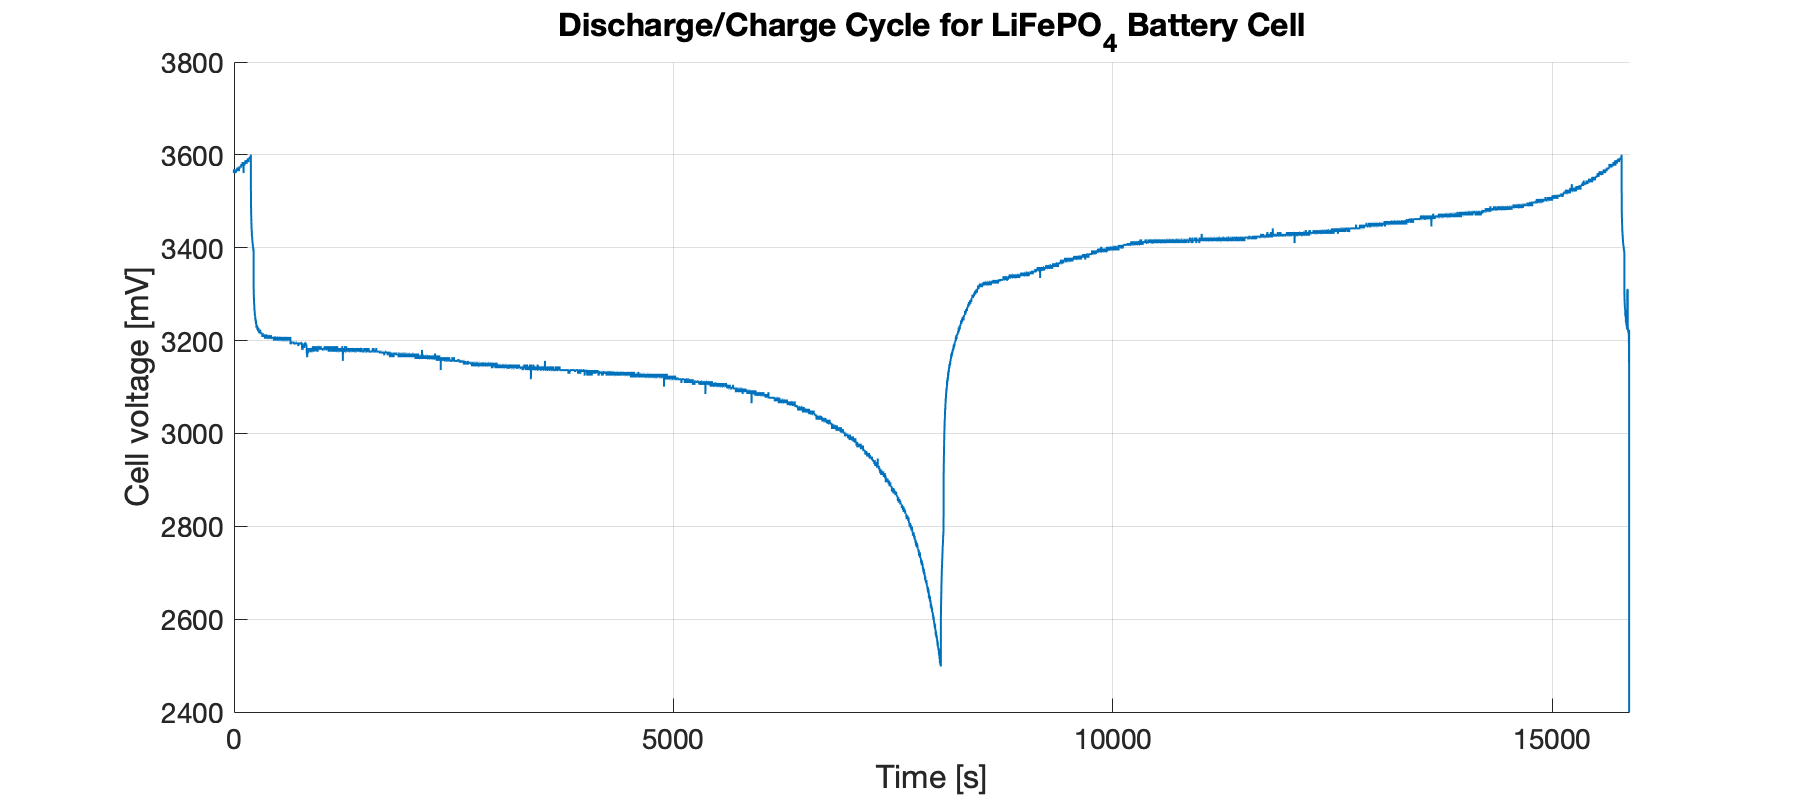
\includegraphics[scale=0.22]{Charge_Cycle2.png}
    \caption{The voltage evolution of a battery cell through a full discharge/charge cycle. The
    cell is fully charged at 200 s and 16000s and fully discharged at 8000s.}
    \label{fig:charge_cycle}
\end{figure}

In addition to logging the cell voltage, the provided charging algorithm also 
logs the charging current. By integrating said current for a full charge or 
discharge section we can determine a cells capacity in mAh. The results from 
performing this analysis on each cell are shown in table \ref{table:1}:

\vspace{5pt}
\begin{table}[h!]
    \centering
    \begin{tabular}{||c| c c c c c||} 
        \hline
        Cell Number& 1 & 2 & 3 & 4 & 5 \\ [0.5ex] 
        \hline
        Capacity (mAh) & 542.7	& 526.1	& 519.5	& 530.1	& 543.7\\ [1ex] 
        \hline
    \end{tabular}
    \caption{Cell capacities}
    \label{table:1}
\end{table}

As expected from the datasheet\cite{batteryDatasheet} all cells have a capacity of about 500 mAh. However, some cells 
have a higher capacity than others, which may have implications for the 
performance for certain battery configurations.

\paragraph*{PV panels}
The PV panels are rated for a maximum power of 1.15 W at a voltage of 
5.0 V and current 230 mA. Away from the maximum power point the performance 
of the panels can be determined from their IV curves. To find the IV 
curves, each panel was connected on the B-side of the SMPS operating 
in non-synchronous boost. They were then lit by the lamp and the duty 
cycle of the SMPS was swept while measurements of panel current and 
voltage were taken. The resulting data was processed and is plotted 
in Figure~\ref{fig:IV_curve}.

\begin{figure}[H]
    \centering
    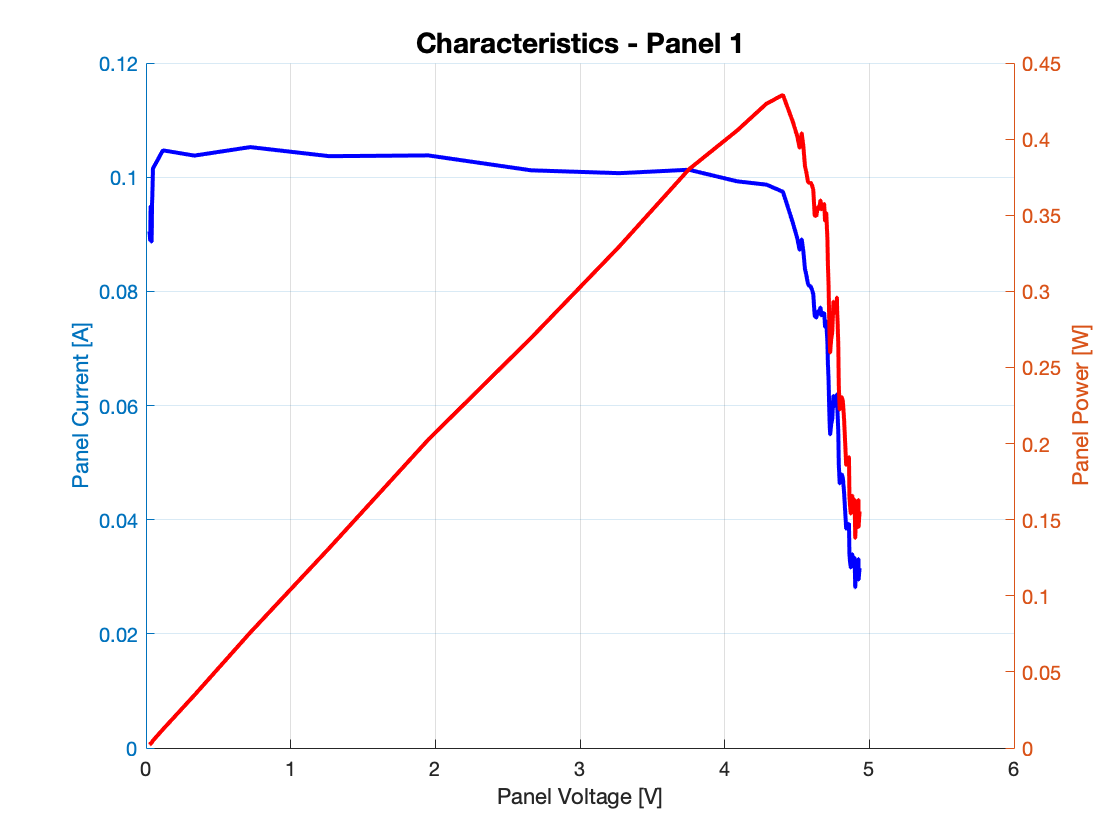
\includegraphics[scale=0.18]{Panel1.png}
    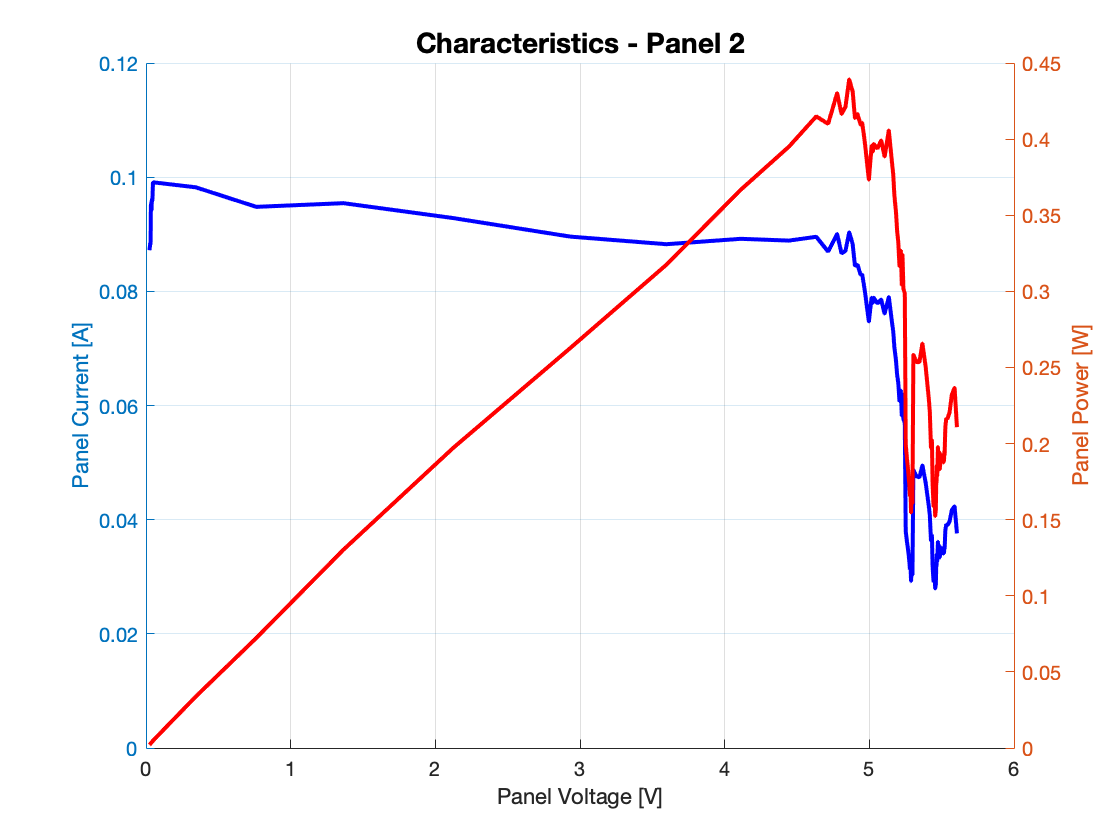
\includegraphics[scale=0.18]{Panel2.png}
    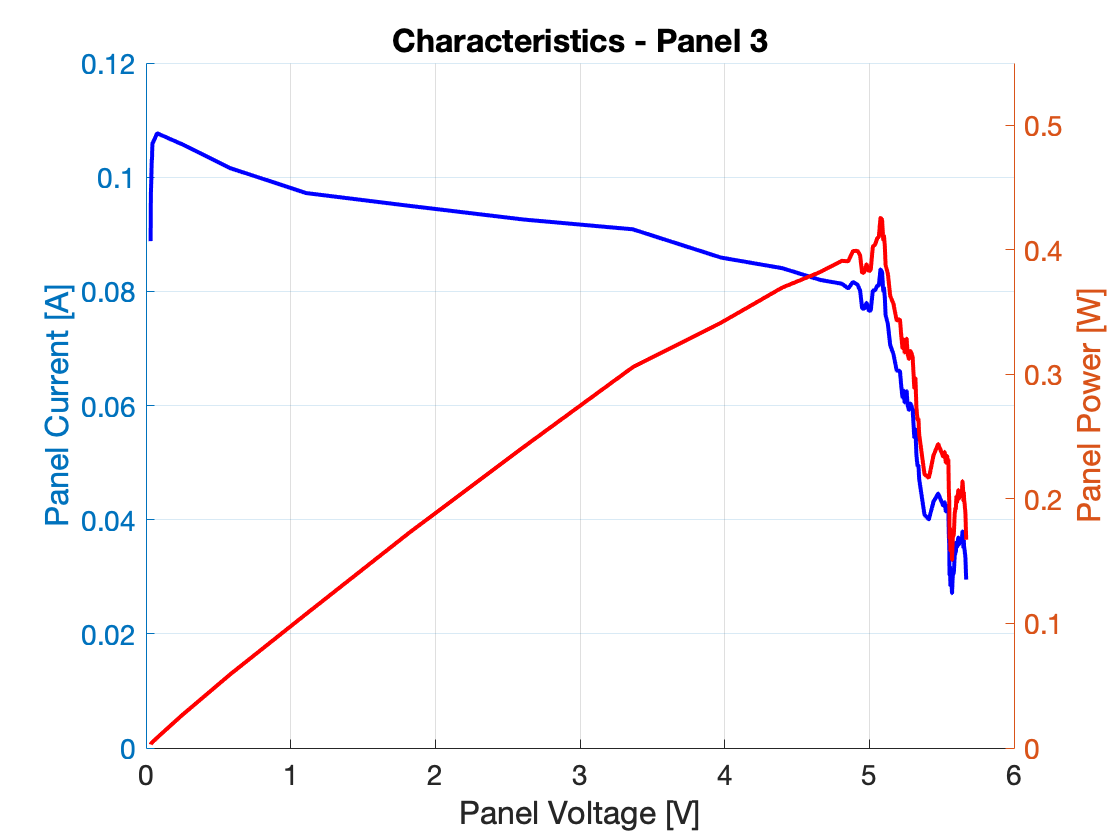
\includegraphics[scale=0.18]{Panel3.png}
    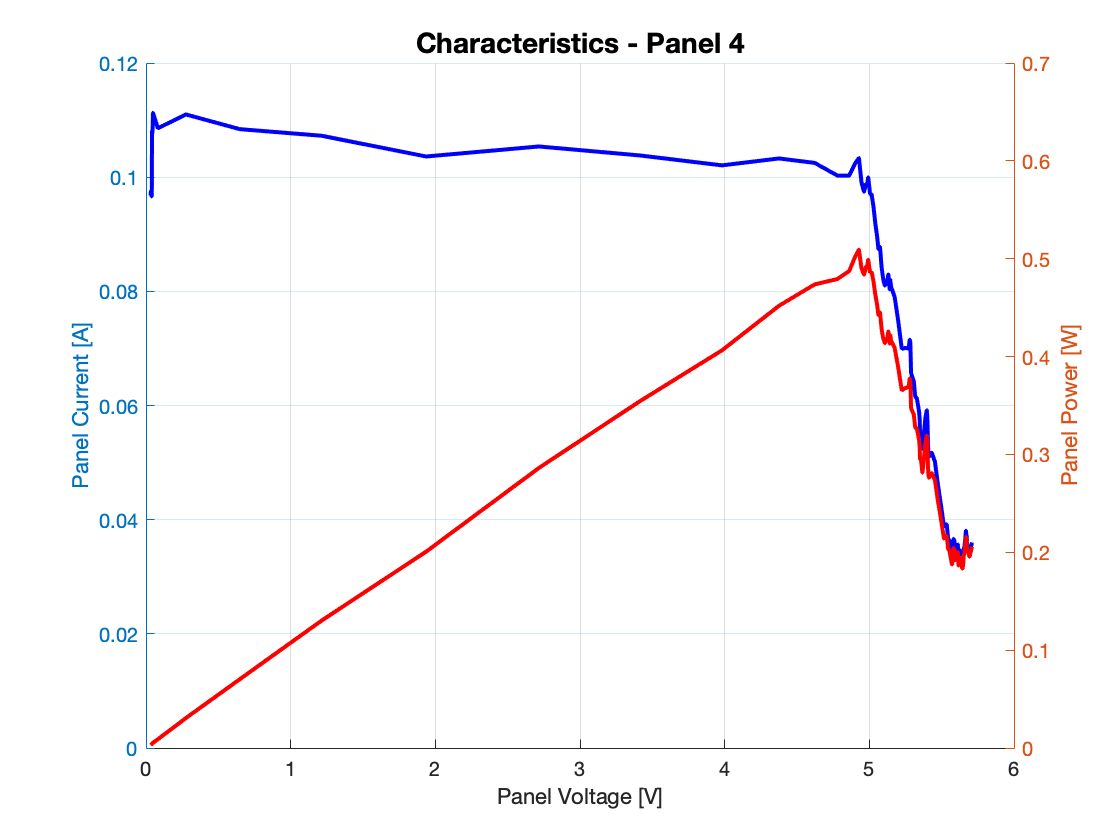
\includegraphics[scale=0.18]{Panel4.png}
    \caption{IV curves for the PV panels.}
    \label{fig:IV_curve}
\end{figure}

Even though the data is noisy, it is clear that all panels exhibit the 
standard IV characteristics of a PV cell. That is, they behave as 
non-ideal current sources with a nearly constant current at low 
voltages and a rapid current reduction at high voltages\cite{green}. 
Moreover, it is clear that the provided lamp activates the panels poorly 
as the peak power for each of the panels is only $\sim$0.5 W.

\paragraph*{SMPS}
\begin{wrapfigure}[12]{r}[0pt]{0.5\textwidth}
    \centering
    \raisebox{0pt}[\dimexpr\height-3\baselineskip\relax]{%
        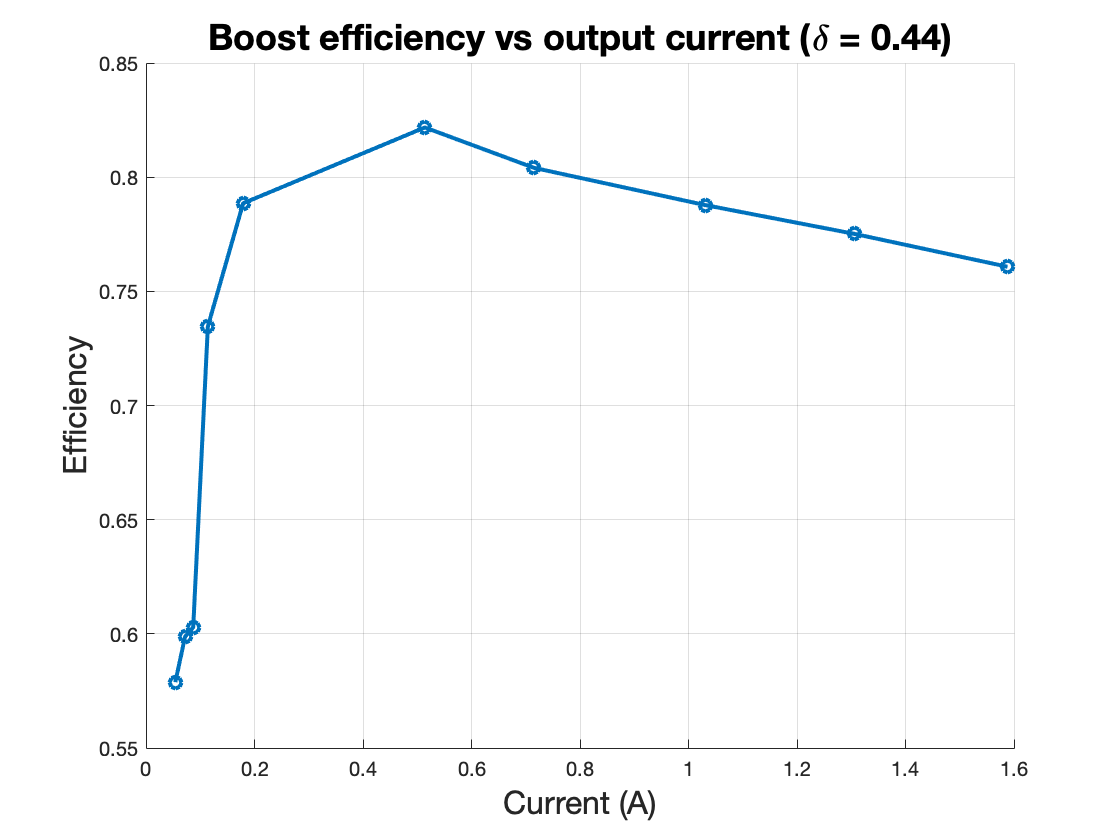
\includegraphics[trim=0pt 0pt 0pt 0pt,width=0.48\textwidth]{Boost_efficiency_wduty.png}
    }%
    \vspace{-5pt}
    \caption{SMPS efficiency versus output current with input voltage of 5V\cite{powerLogbook}}
    \label{fig:efficiency}
\end{wrapfigure}
The SMPS is rated for 10 W throughput with a maximum boost output voltage 
of 35 V and maximum output current of 10 A\cite{SMPS_lab}. These ratings 
are far higher than what is needed to charge the battery and are not 
expected to impose limitations on the design of the energy module. 

The many characteristics of the SMPS have been thoroughly examined in 
2nd year labs. However, for the energy submodule the most important 
characteristic will be the SMPS efficiency during non-synchronous 
boost operation. A graph of efficiency versus output current is shown 
in Figure~\ref{fig:efficiency}.

\subsubsection{Initial Design}

\paragraph*{Battery Configuration}
When designing the battery pack there are two principal choices that need to be 
made. Firstly, how many cells should be in the battery pack and secondly, in 
what manner should these cells be connected? 

The optimal number of cells is in large part set by the power and energy 
needs of other submodules. During testing the total power draw of the 
rover was found to be about 2 W. Each battery cell has a nominal voltage 
of 3.2 V and a maximum peak discharge current of 1 A \cite{batteryDatasheet}, 
giving a maximum power draw of 3.2 W per cell. Thus, even with only a 
single cell the power requirements of the rover are met. However, each 
cell can only store about 
\(3.2 \unit{V} * 0.5 \unit{A} * 3600 \unit{s} \approx 5760 \unit{J} \),  
which would only power the rover for 48 minutes. It is desirable to 
have the rover be operational for as many hours as possible each day. 
Assuming that 12 hours a day are completely without sunlight it is 
clear that the rover cannot work through the night even if all 
5 available battery cells are used. To give the rover the most 
operational hours we would then want to use all 5 battery cells. 
However, connecting 5 battery boards to the Arduino would use at 
least 11 of the 12 free Arduino pins, leaving only one pin for 
all other purposes. As such it might be wise to not use all of the 
available cells in the battery pack.

Now consider the PV array. Each PV panel is rated for 1.15 W, meaning that 
the array as a whole should have a peak power of 4.6 W. As shown in 
Figure~\ref{fig:efficiency} the peak efficiency of the SMPS in boost mode 
is about 80\% giving a maximum usable power on the SMPS output of 
\(0.8 * 4.6 \unit{W} \approx 3.7 \unit{W} \). Assuming 12 hours of 
sunlight in a day, this means that the PV array produces less energy 
each day than the rover uses in 24 hours. It is therefore of high 
priority to capture as much of the solar power as possible. The 
battery cells have a standard charging current of  250 mA 
\cite{batteryDatasheet}. The power needed to charge the battery 
pack at this current based on the number of cells is shown in 
table \ref{table:2}. 

\vspace{5pt}
\begin{table}[h!]
    \centering
    \begin{tabular}{||c| c c c c c||} 
        \hline
        Number of cells& 1 & 2 & 3 & 4 & 5 \\ [0.5ex] 
        \hline
        Nominal charging power (W) & 0.8 & 1.6 & 2.4 & 3.2 & 4.0\\ [1ex] 
        \hline
        Peak charging power (W) & 0.9 & 1.8 & 2.7 & 3.6 & 4.5 \\ [1ex] 
        \hline
    \end{tabular}
    \caption{Power needed to charge at standard charging current at nominal cell voltage of 3.2 V and peak cell voltage of 3.6 V}
    \label{table:2}
\end{table}
From the table we see that a battery pack using 4 cells has the highest 
power consumption without going over the limit of 3.7 W. Moreover, 
4 cells is a good compromise between having enough free Arduino 
pins and providing enough energy for long operation. As such,
a 4 cell battery pack seems like a good choice. Moreover, as cells 
1, 2, 4 and 5 were found to have the highest capacity, these 
are the cells that will be used. 

There are several ways to connect the 4 cells into a power pack, 
however the design brief advised against mixing parallel and series 
connections\cite{energyBrief}. As such only fully series and parallel 
battery packs will be considered. 

A series battery pack has some obvious disadvantages compared to 
a parallel battery pack. Firstly, for a series battery pack the 
battery capacity is limited by the weakest cell. This is not the 
case for a parallel battery pack as it is possible to draw different 
currents from each cell. As a consequence, a series battery pack
is able to store less usable energy than an equivalent parallel 
battery pack. Moreover, to check the OCV of each cell they need 
to be switched out of circuit using the battery board relay. 
For a series battery pack this leads to an open circuit and 
any charging/discharging must halt while the voltage is measured. 
For a parallel battery pack on the other hand, switching the 
relay of a cell only takes that one cell out of circuit and it 
is still possible to charge/discharge while measuring cell 
voltages. Finally, a parallel battery pack is 
self-balancing\cite{batteryBalancing}, while series cells 
need to be manually balanced using, for example, balancing 
resistors. This not only is more complex, but also leads to 
energy being lost as heat during balancing.

There is however a major weakness to a parallel battery pack: it is 
very hard to track the current into individual cells. The current 
sensor on the SMPS can only measure the current flowing into the 
battery pack as a whole and there is no way to know how the 
current splits between cells. To prevent over-current one must 
therefore operate with the assumption that all the current can 
flow into a single cell. Each cell is only rated for a max charging 
current of 500 mA\cite{batteryDatasheet}, which is therefore the 
maximum charging current. At 500 mA the nominal charge power is 
only \(3.2 \unit{V} * 0.5 \unit{A} = 1.6 \unit{W} \), which is 
less than half the available solar power and with a parallel 
battery pack a lot of power will therefore go unused. As 
previously determined, energy is a precious resource and only 
being able to use half of the available solar power is such a 
large drawback, that despite the disadvantages of a series battery 
pack it is still deemed the best option.

\paragraph*{PV Array Configuration}
There are four ways in which the four PV panels can feasibly be connected. 
The possible arrangements are shown in Figure~\ref{fig:arrayConfigurations}.

\begin{figure}[H]
    \centering
    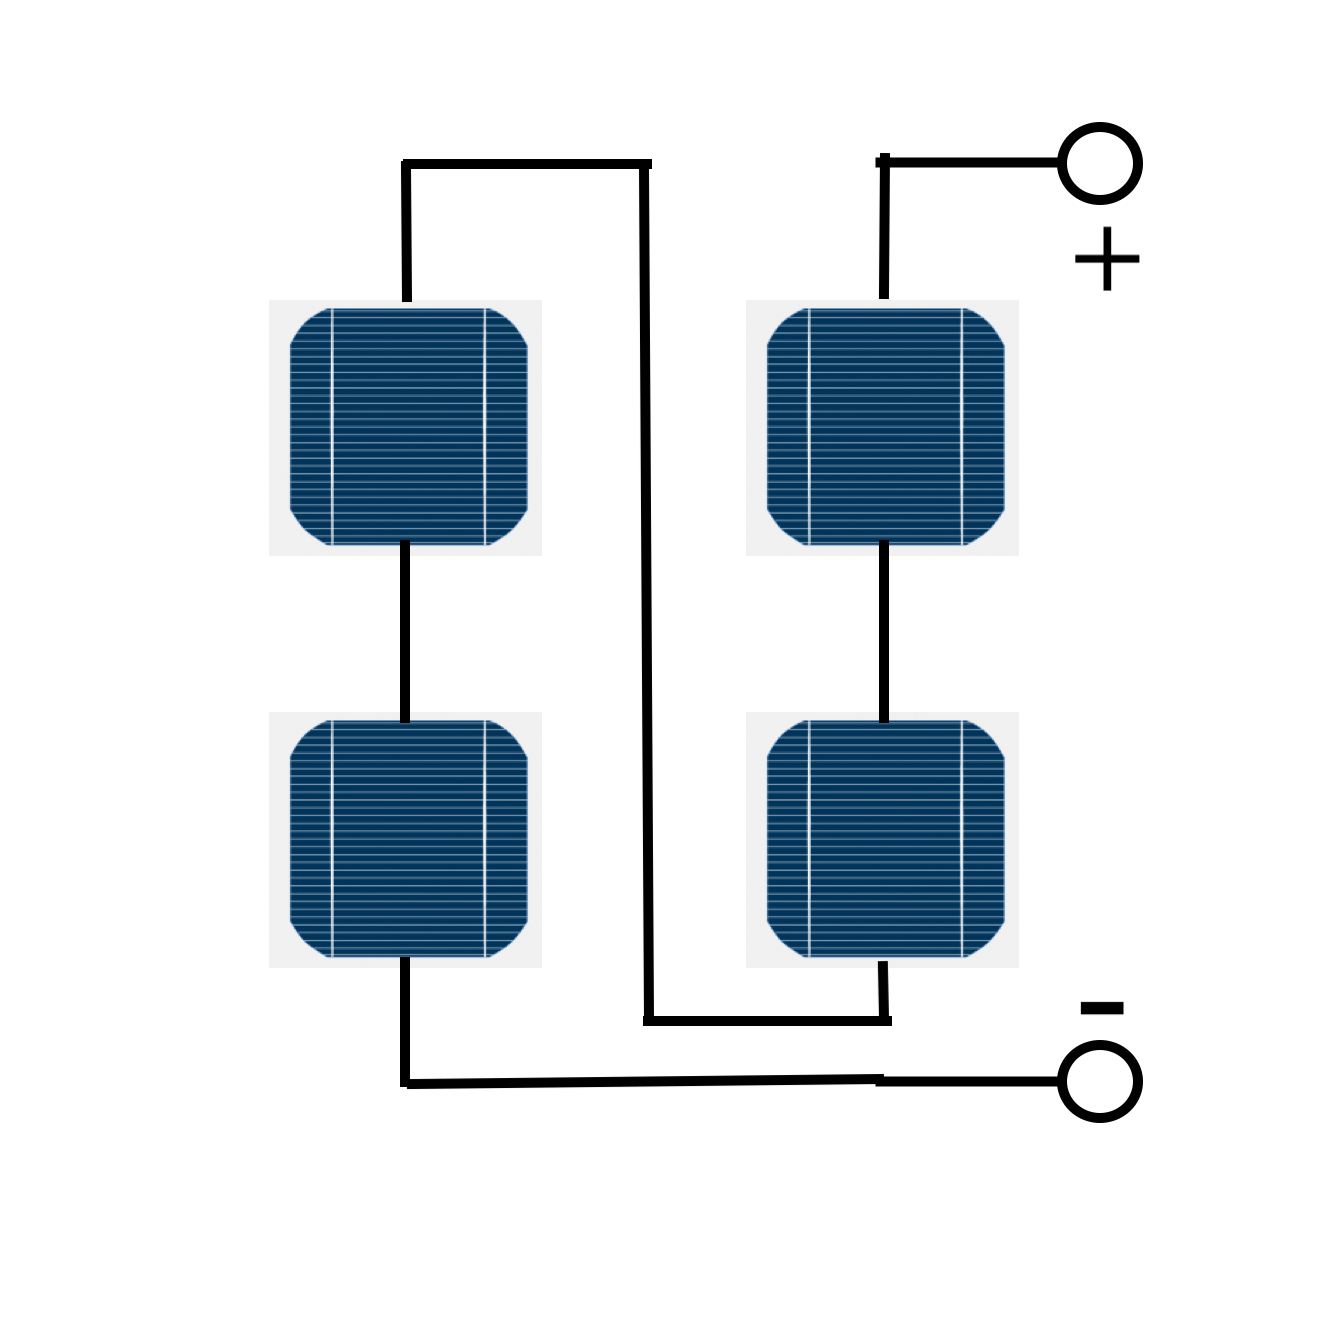
\includegraphics[scale=0.10]{Series(S)}
    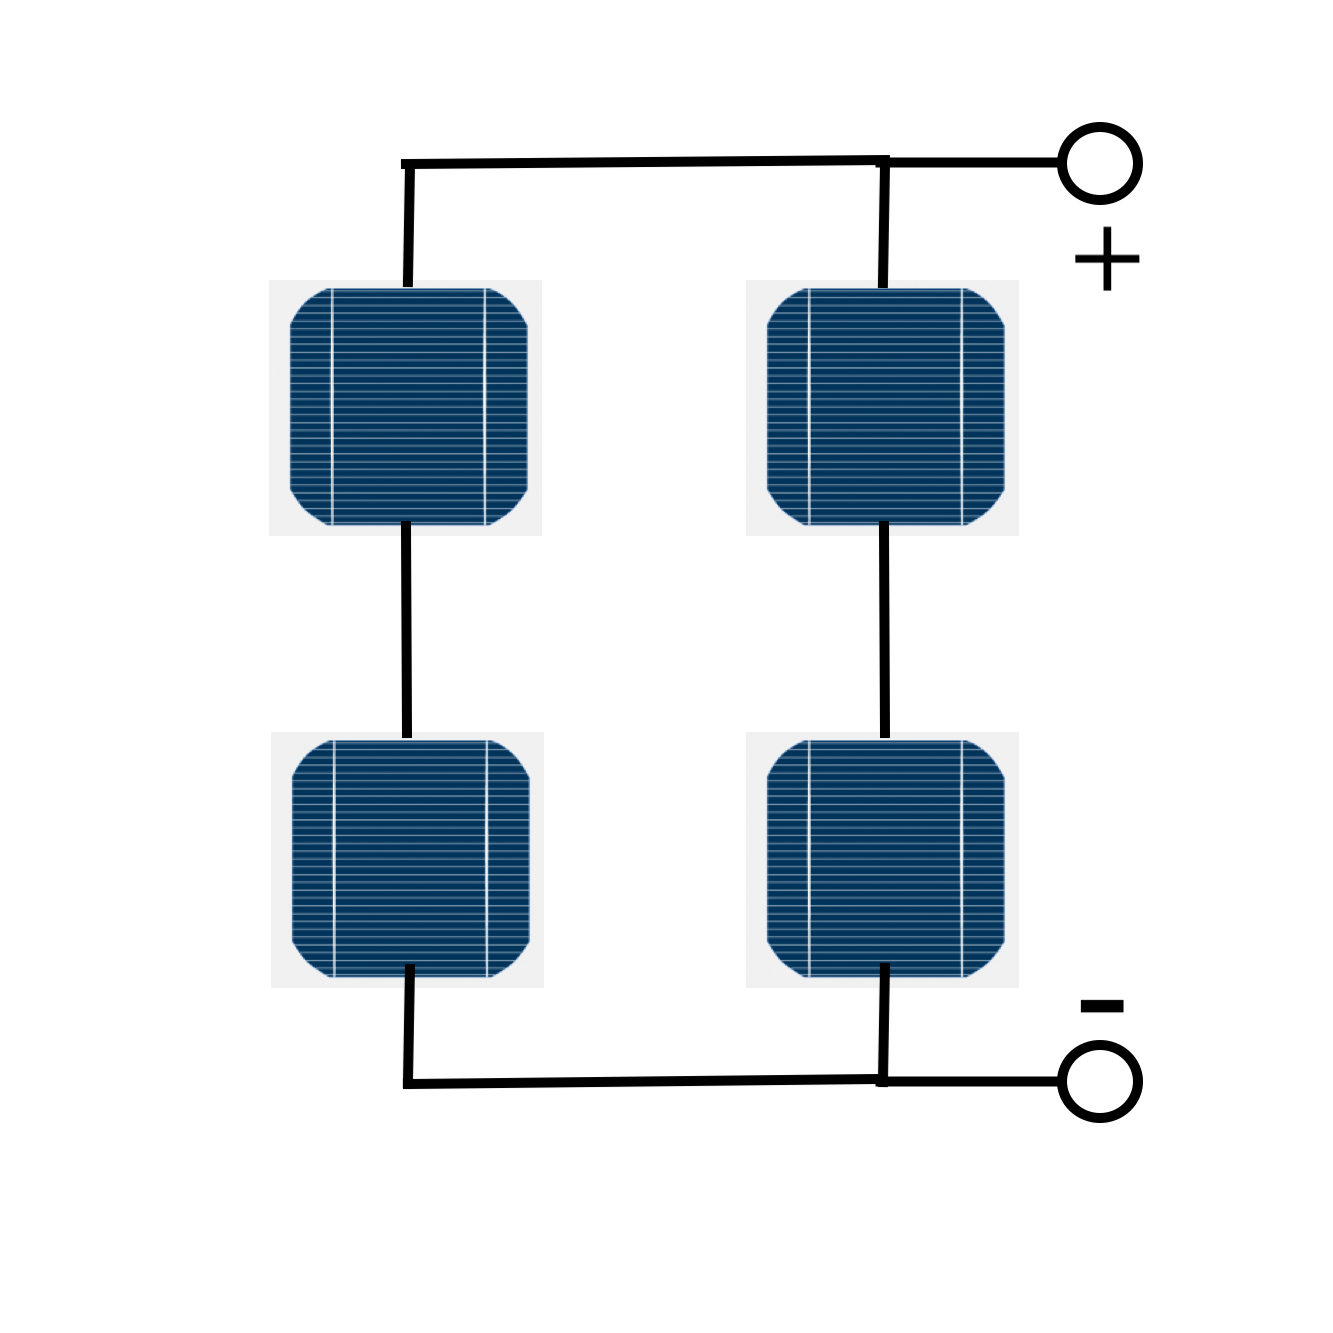
\includegraphics[scale=0.10]{Series-parallel(SP)}
    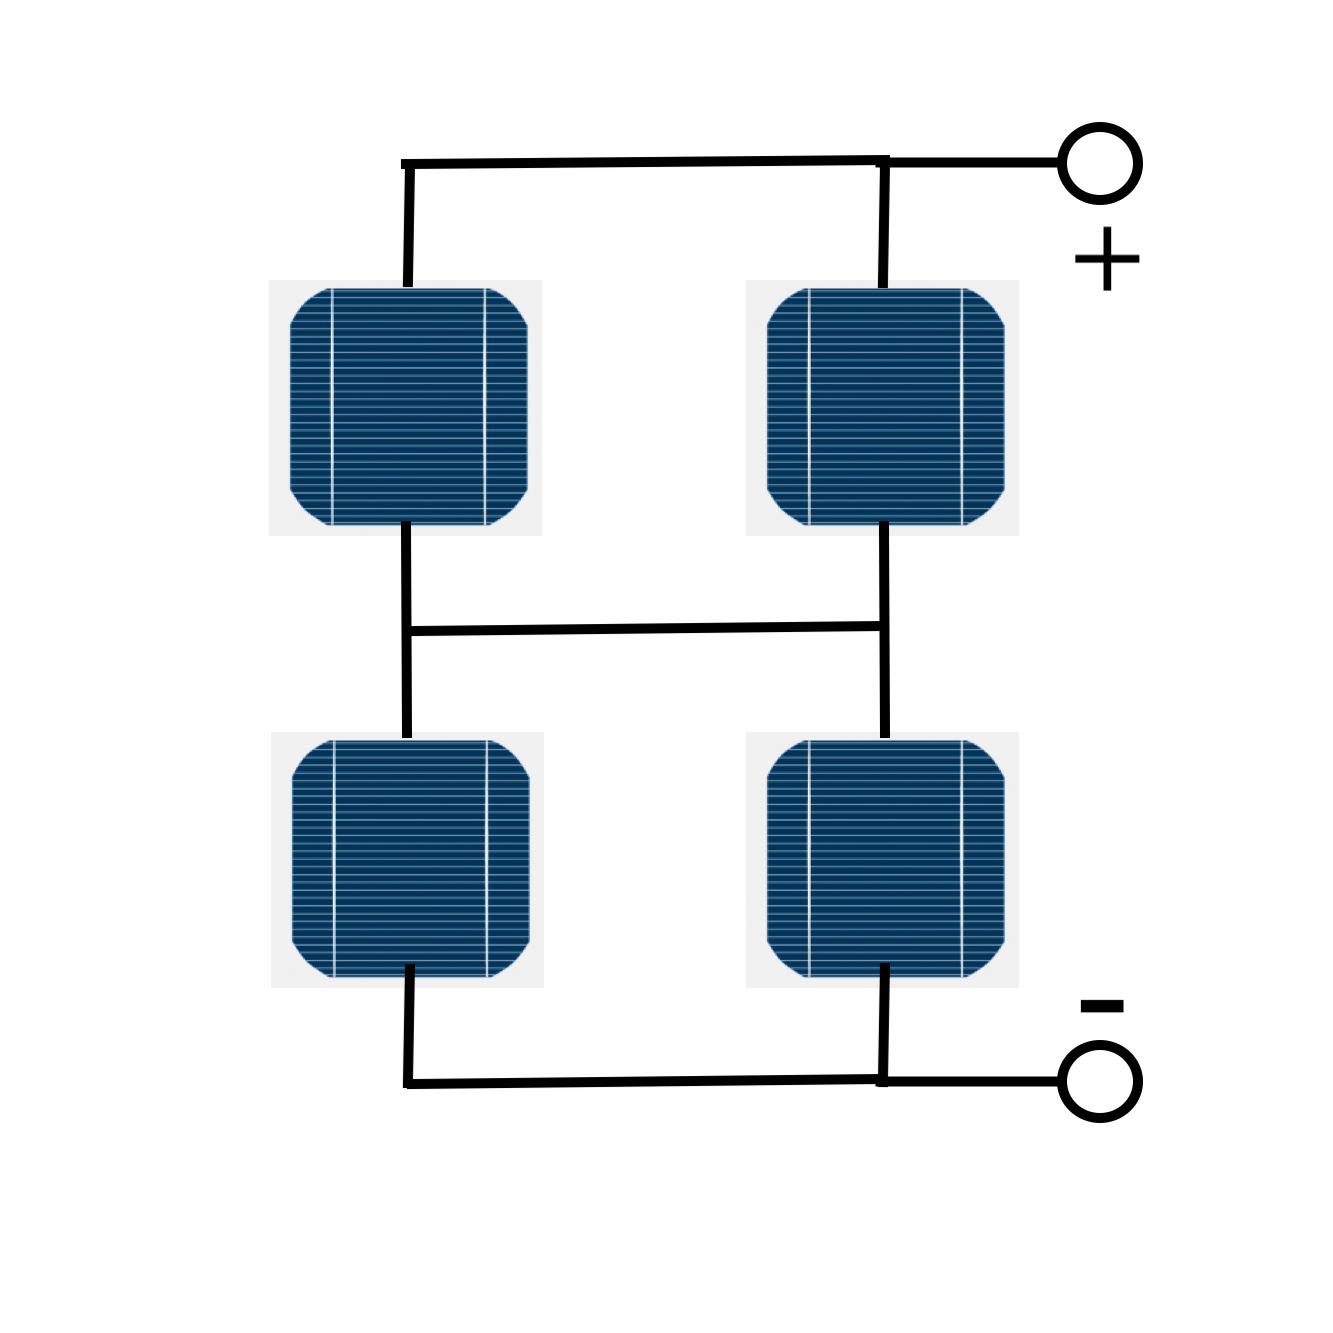
\includegraphics[scale=0.10]{Total-cross-tied(TCT)}
    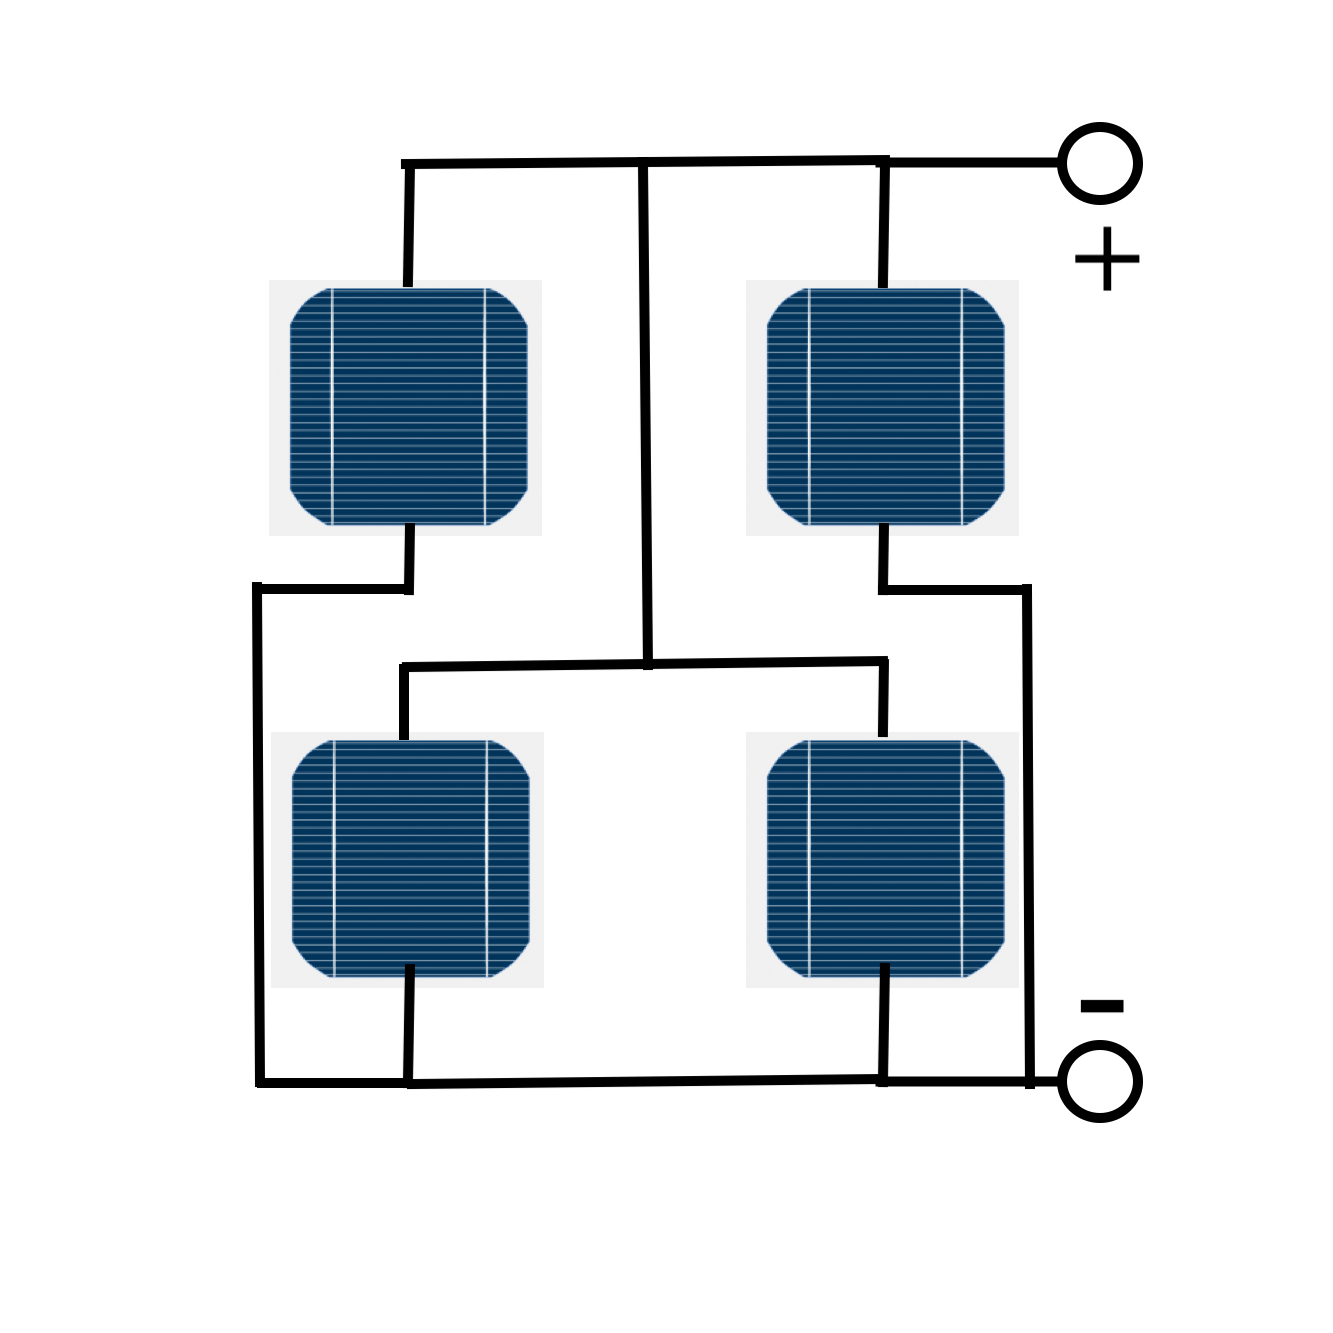
\includegraphics[scale=0.10]{Parallel(P)}
    \vspace{-10pt}
    \caption{From left to right: Series (S), Series-Parallel (SP), Total-Cross-Tied (TCT), Parallel (P)}
    \vspace{-10pt}
    \label{fig:arrayConfigurations}
\end{figure}
Consider first a pure series connection. During characterisation each PV 
panel was found to have a max voltage of  $\sim$5.5 V. In a series 
connection the array voltage will then be 20+ V. The nominal voltage of 
the series battery pack is \(4 * 3.2 \unit{V} = 12.8 \unit{V} \). As the 
array voltage is higher than the battery voltage, the SMPS must be used 
in the buck configuration. However, the maximum buck input voltage is 
only 7 V\cite{PMOS} and therefore a series connected PV array cannot be 
used. Similarly, for the Series-Parallel and Total-Cross-Tied arrangements 
the maximum array voltage will be about 11 V. However, as the battery 
voltage can swing between 10 V and 14.4 in a charge cycle, neither a 
buck nor a boost configuration will be able be able to provide the 
necessary voltage range with an 11 V input voltages. Thus it is not 
possible to use either the Series-Parallel or Total-Cross-Tied 
configuration. This leaves a purely parallel connected PV array as 
the only viable option, which is why it has been chosen. 

\paragraph*{Maximum Power Point Tracking}
The energy submodule only has access to a single SMPS device. At any time it 
will therefore only be possible to either perform MPPT or have the PV power 
be outputted at the correct current/voltage. This is not a problem, as the 
goal of the PV array is not to output the maximum amount of power, but simply 
to provide the power demanded by the charging algorithm. As such, the system 
does not need conventional MPPT. However, if the PV panels cannot provide the 
demanded power some sort of power tracking must be used. 

\begin{wrapfigure}[20]{r}[0pt]{0.45\textwidth}
    \begin{center}
        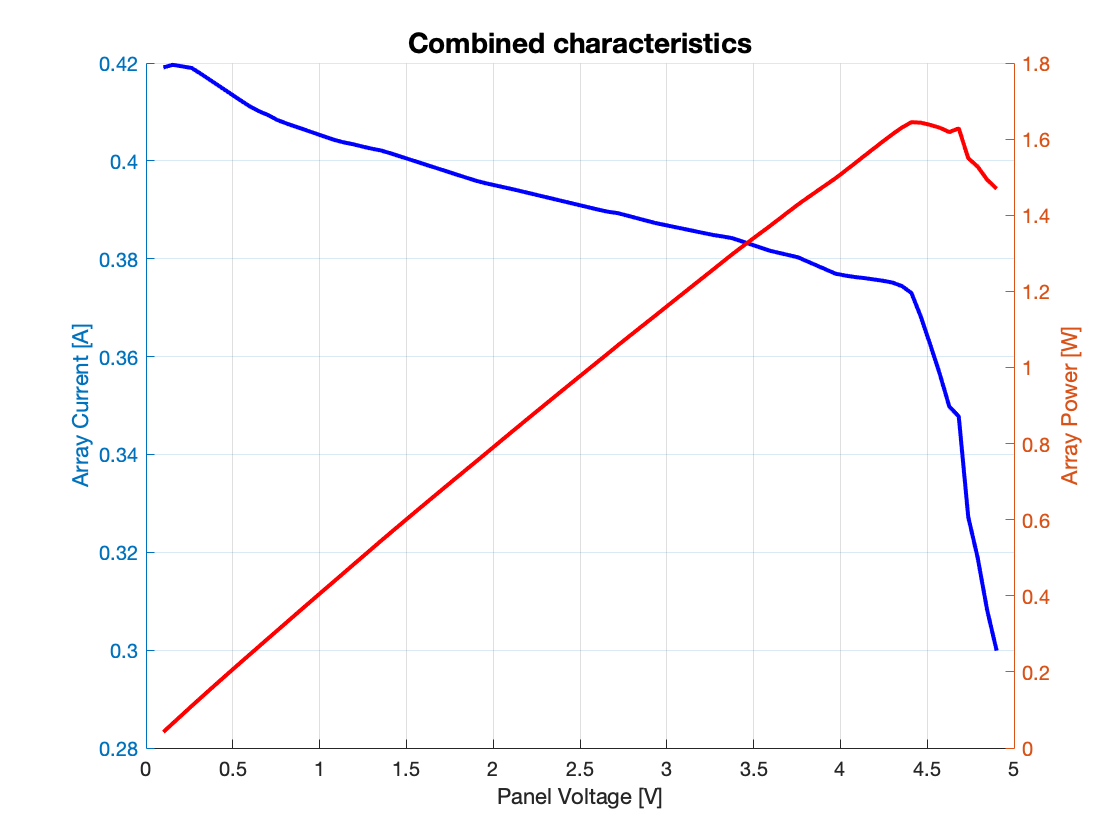
\includegraphics[width=0.45\textwidth]{Combined.png}
    \vspace{-15pt}
    \end{center}
    \caption{IV-curve (blue) and power curve (red) of the parallel configured PV array lit by a lamp.}
    \label{fig:parallelArray}
\end{wrapfigure}

Consider an SMPS being used to charge a battery pack at a set current. If 
the actual current on the output is lower than the setpoint, one would 
attempt to increase the output current by increasing the output voltage. 
This is achieved by increasing the duty cycle. Similarly, if the output 
current is too high one would attempt to lower the output current by 
lowering the duty cycle. From these considerations we see that increasing 
and decreasing the duty cycle is associated with higher and lower output power 
respectively. Now compare this with the IV and power characteristics of the 
parallel PV array shown in Figure ~\ref{fig:parallelArray}. For an SMPS, 
increasing the duty cycle will lower the input resistance, causing the input 
current to increase. As increasing the duty cycle increases the output 
power so too must increased input current lead to increased input power for 
an equilibrium to exist. However, increased input current only gives increased 
output current if the PV panels are operating in the region to the right of the 
maximum power point. Thus this is the region one would want the panels to operate in. 

\paragraph*{State of Charge}
The state of charge (SOC) of a battery is defined as the remaining usable charge 
given as a percentage of the battery’s total charge capacity\cite{DICKINSON2009452}. There are many 
methods for  estimating the SOC of a battery, the most common of which rely on 
measurements of the voltage and/or current of the battery\cite{DANKO2019186}. The perhaps 
simplest SOC estimation method is to measure the open circuit voltage (OCV) 
of the battery and then calculate the SOC using a formula or a lookup table. 
For many types of battery this is a good estimation method. An example is 
lead-acid batteries, for which the OCV varies approximately linearly with the 
SOC. However, as was shown figure ~\ref{fig:efficiency}, this is not the case 
for LiFePO4 batteries. For LiFePO4 cells the voltage is nearly constant for 
a majority of each charge/discharge cycle. Any measurement error or change in 
OCV due to current recently flowing through the battery, would therefore produce large 
SOC estimation errors. This holds true for all SOC methods relying purely on 
voltage measurements and they are therefore not good alternatives. 

An alternative SOC estimation method is Coulomb counting, where the current 
flowing through the battery is integrated to find the net charge that has 
left or entered the battery. Seeing as charge is a conserved quantity nearly 
all charge put into the battery will be available during discharge. As such, 
the SOC will vary nearly perfectly linearly with the integrated current. 
The sources of error for Coulomb counting are mainly the Coulombic efficiency 
of the batteries and current measurement errors. However, using correction 
methods the error can be kept small, on the order of 1-2\%\cite{NG20091506}. Given the 
simplicity of the estimation method, this is a very small error. Other 
estimation methods, such as Kalman filters and neural networks, are claimed 
to give higher estimation accuracies\cite{DANKO2019186}. However given the already high 
accuracy of Coulomb counting the improvement is marginal. Moreover, they 
are far more complex both computationally and in implementation. As such, 
Coulomb counting was deemed the best option for SOC estimation. 

\paragraph*{State of Health}
The state of health of a battery is a measure of its current condition and 
performance compared to when it was new\cite{mpower}. Indicators of a battery’s 
state of health include battery charge capacity, energy capacity, cell voltage 
balance, and the number of completed charge/discharge 
cycles\cite{https://doi.org/10.1002/er.3598}. Over the course of its lifetime 
the SOH of a battery will naturally degrade. However, through SOH maintenance 
the degradation can be slowed significantly. Most importantly for a series 
battery pack is to keep the battery cells balanced, as unbalanced battery 
cells lead to lower capacity and faster cell degradation\cite{texas}. To 
facilitate balancing, each of the provided battery boards have mounted 
resistors which through a MOSFET can be connected to the battery cell. During 
operation one must decide when to switch said resistors on and off to keep the 
cells balanced. Usually, balancing is only done towards the end of a charge cycle. 
There are several reasons for this. Firstly, passive balancing requires energy 
to be expended and will therefore reduce the total amount of usable energy 
in a battery if done during discharging. Secondly, differences in impedance 
and charge curves between cells might make it look as though a cell is charged 
more than others, but the voltage difference might disappear naturally as the 
battery is charged more or as charge current is reduced towards the end of a 
charge cycle.

\paragraph*{Integration of the Energy Submodule}
It is not necessary to physically integrate the energy module with 
the full rover. However, if it were, the energy module could either 
be integrated as a charging station or be mounted directly on the 
rover itself. The advantage of a charging station is that the 
battery is only ever charged or discharged at a given time. This 
makes it easier to track current and power and leads to simpler 
charging and SOC algorithms. A drawback of using a charging station 
is a reduced range, as the rover always needs to get back to the 
charging station before its battery is depleted. Moreover, if the 
rover is detached it is difficult for the energy module to track 
the cell voltages and SOC during discharging. This could be fixed 
by using the microcontroller of another subsystem to track the 
battery while the rover is not connected to the charging station. 
However, a likely simpler solution is to mount the energy module on 
the rover. This would increase range, but does require the battery 
to charge and discharge at the same time. To be able to track the 
battery current, it would then be necessary to collect current and 
power data from other submodules. This data could be relayed through 
control and read in on the energy Arduino through UART.

The rover has four separate voltage regions. The battery and PV array 
have already been discussed. In addition there is a 5 V node used to 
power the FPGA and microcontrollers, and a variable voltage node used 
to power the motors. This power must originate in the battery and as 
such the 5 V and motor voltages must be connected to the battery 
through voltage converters. The obvious implementation is to use 
two switch mode power supplies in buck mode, one to provide 5 V and 
one to power the motors. One problem exists however with this solution: 
The 10.0 – 14.4 V of the battery is higher than the SMPS maximum 
input voltage\cite{powerLogbook}. A way to solve this would be to 
exchange the PMOS on the SMPS board for another NMOS, which would 
increase the maximum input voltage.

%End of energy functional section

%End of funtional section



\section{Implementation}

\subsection{Control} 

\subsubsection{Command Communication}

The first connection that had to be established was the one between Command 
and Control. From the requirements set out, it was clear that the ESP32 
had to use it’s WiFi capabilities to interface with Command. The two 
options available to the ESP32 are as follows: to act as either it's own 
router through the Access Point mode or it's own station under an existing 
router through the Stationary mode \cite{ESPWIFI}. As the Access Point mode 
would mean that the rover is not connected to the internet, since 
it would create a private inaccessible network, the stationary mode was chosen 
instead. Having the capability to communicate with the rover through an 
existing router allows for communication from anywhere in the world 
through WiFi. This would be much more flexible and representative of 
communicating with a rover on Mars. A working prototype for communication 
was built using TCP. In order to test whether it was functioning, since 
Command was still in very early stages, a python-based TCP server was created. 
When running, it would take the text put into the terminal and send it 
to the ESP32 while displaying the messages incoming from the ESP32. 
The ESP32 was configured to echo back all messages. Through this 
simple system, the connection was successfully implemented by debugging
 the connection and the messages being sent back and forth.

\subsubsection{Drive Communication}

As the first physical connection between the ESP32 and a peer 
microcontroller, it was decided that the best course of action would 
be to completely test communication with the simplest of devices, 
the Arduino Nano Every. Since the Arduino has an extensive 
and well-documented library for UART communication, Drive was the 
best subsystem to test out initial communication. When testing out the 
UART communication, two methods documented through the Arduino IDE were used. 
SoftwareSerial \cite{ESPSoftwareSerial}, which uses code to imitate a 
UART connection allowing you to map the peripheral to any GPIO pin, 
or directly assigning the pins through hardware assignment. 
Initially the former was utilised, but it was quickly realised that the 
multiplexing feature of the ESP32 chip allows for hardware configuration 
to most of the GPIO pins of your own choice \cite{ESP32PinOut}. However, 
an interesting interaction that was recorded was that the 3 UART connections 
that are available to the ESP32 aren’t completely unused \cite{ESPHardwareUART}. 
One of the UART connections is used to communicate with the laptop when 
connected via USB. This UART connection by default is assigned to pins 
0\_RX and 1\_TX on the Arduino Adapter Board. As a result, 
mapping a secondary UART on these same pins and serially writing 
to your laptop would also write to the peripheral connected to 
0\_RX and 1\_TX. Once this was determined, these two pins were 
discarded as options for communication. UART between Drive and Control 
was tested with some movement functionality on Drive and test code on the 
ESP32 allowing for commands to be sent by the terminal of the 
Serial Monitor through the UART connection between the laptop and the 
ESP32. This was then forwarded to Drive. This allowed for imitating the 
entire chain of communication from Command to Drive, but by only using the 
Control subsystem and ESP32 as a testing device.

\subsubsection{Vision Communication}

As described in the functional requirements for Control, the initial 
design was to set up two SPI connections with the FPGA due to the 
overabundance of pins between the two devices. SPI as a peripheral was 
superior as well since it would take less overhead for the FPGA and 
would be a faster method for communication when compared to UART 
\cite{CommProtocolComp}. Alongside this, due to the ESP32 being dual-core
, a task scheduler \cite{ESP32DualCore} could be used to simultaneously support 
image transfer while standard data was being transferred. Initially, to test out 
the SPI capabilities of the ESP32, the ESP32 was set up as an SPI controller, 
while an Arduino was set up as an SPI peripheral. Through SPI.h, 
a library designed for the ESP32 and ESP8266 \cite{ESP32ArduinoGithub}, 
this was accomplished and communication between the two 
devices was successful. It was discovered that although the Nios\textsuperscript{\textregistered} II processor 
supported acting as an SPI controller, acting as an SPI peripheral was not 
well-supported. This proved problematic when instantiating an SPI peripheral 
using the Nios\textsuperscript{\textregistered} II, even if the FPGA itself supported it. Although there is an 
immense amount of support for the ESP32 on the Arduino, when it comes 
to acting as an SPI peripheral, this has yet to be implemented from the 
Espressif documentation in C. Although SPI peripheral libraries have 
been created for the older ESP8266, this unfortunately has not extended 
to the ESP32. There have been some projects which attempted to develop 
and use their own SPI peripheral functionality. This is done by 
translating and porting over the libraries from the original Espressif 
documentation into Arduino, setting them up as Arduino libraries. 
After attempting to rework these libraries \cite{ESPSPISlaveMaster} \cite{ESPSPISlave}so that they could support 
the functionality we needed, it was eventually discarded as an option. 
Even if the ESP32 could function successfully as an SPI controller, 
it wouldn’t matter since the FPGA had the same limitation as it only 
had SPI controller functionality. Eventually it was agreed that this 
would have to change to UART for standard data transmission. 
As for image transfer, since this was meant to be done through SPI, a 
framework for the ESP32 acting as an SPI controller to transfer these 
images was created. However, as it proved too difficult to use the FPGA 
as a functioning SPI peripheral, this also had to be scrapped. In the 
end the only connection which remained between Vision and Control was 
the singular UART port designed for collecting Vision data to send to 
Command for mapping and detecting obstacles.

\subsubsection{Integrating Communication}
 
Although the communication between peer devices was successfully set
up and tested, there was still a small challenge. To be able to
incorporate all communication such that it could occur simultaneously and
effectively, with as limited of a delay as possible. In order to achieve
this, it was noted that the UART and TCP communication between devices
are always held within internal buffers and as such there is no need to
immediately pull out the data as it arrives. A secondary set of buffers
were created, except these were created to store the next line of data or
next command depending on the datastream. To understand what was considered
a line of data or command, there was discussion between the groups. This
allowed us to dedicate certain characters as “start” and “end” characters
to differentiate between data sets. Also, certain subsystems would send
special characters to the ESP32 to designate their status. For example,
Drive would send an ‘@’ if it was prepared for its next command. Command
would send a ‘S’ if it required the Drive subsystem to stop it’s current
command. Unlike a complete path, which had the program collect the data
from one device and immediately send it to another, this would allow the
program for a better scheduling of tasks to be able to simultaneously keep
up data collection. Once a certain buffer had the required contents to be
sent, a boolean would evaluate to true, activating the sending loop to
transmit the contents of the buffer and then clear it. In the end, this
would allow for staggered sending and receiving between subsystems, giving
the illusion that communication is simultaneous even when all subsystems
are transmitting across the ESP32. For ease of understanding in what order
the processes were occurring, the UART dedicated to Energy was used as a
debugging tool, sending data to the Serial Monitor to understand how the
data was flowing to and from the ESP32.

\subsection{Command}

\subsection{Drive}

\textbf{General Specifications}

Initially, the main goal of the driving subsystem was to make a movable rover. 
The specifications and the limitations of the SMPS, Arduino and the DC motors, 
needed to be known.  The first challenge was to find a way to measure the 
rotations per minute (RPM) of the DC motors, precisely. The solution was to 
stick a small piece of paper on the rotating axes of the DC motor. Additionally,
one screwdriver was placed perpendicularly to the small piece of paper. This was
done because each time the DC motor completed one whole rotation the small piece
of paper would ``trigger'' the screwdriver and generate a distinctive sound.
Finally, the only unsolved part was how to pick up that sound. So, the 
microphone of one set of earphones was placed close enough to the DC motor in order 
to pick up that distinctive sound. Then, the whole process was recorded, leading 
to the following outstanding outcome. The recorded sound was processed with an 
audio application and every time the DC motor completed a whole period the 
waveform of the recorded sound had a spike with a recognisable magnitude. 
Finally, the time difference between one spike to the following one was the 
period (T) of the DC motor. 
Then only the conversion from time to RPM was left and in order to find the RPM,
the following formula was used: \( RPM=\frac{60}{T} \) 

%%%%%%%%%%%%%%%%%%%% Figure/Image No: 1 starts here %%%%%%%%%%%%%%%%%%%%

\begin{figure}[H]
\begin{Center}
\advance\leftskip 0.23in		
    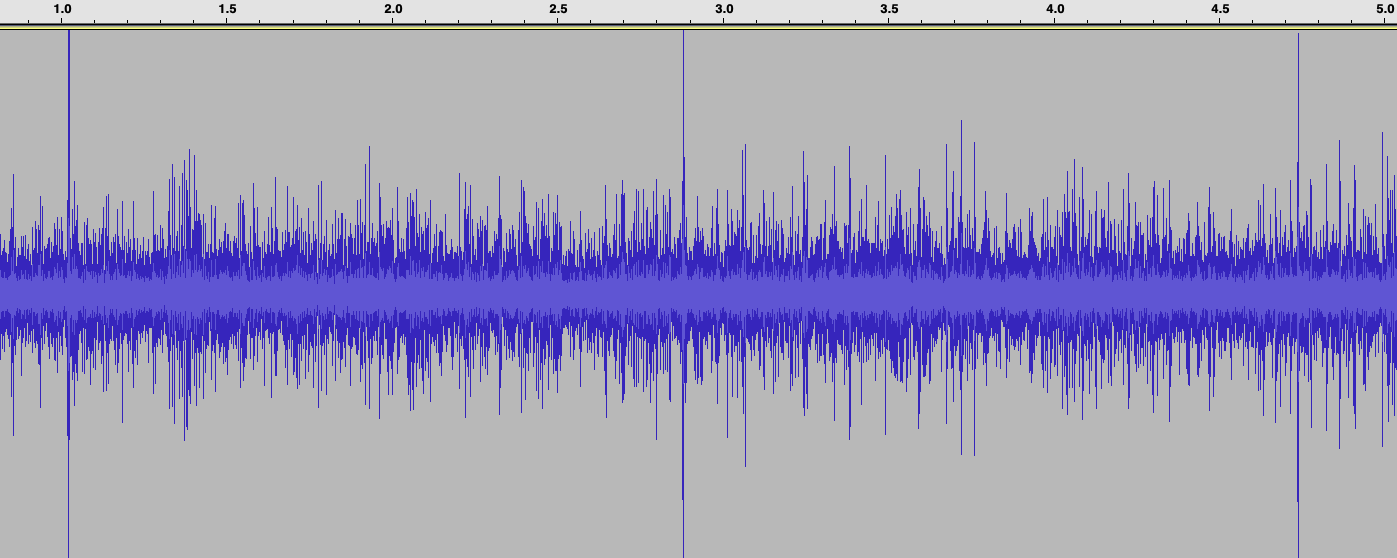
\includegraphics[width=5.06in,height=2.02in]{./media/image2.png}
	\caption{Shows the spikes that correspond to a period(T)}
		\label{Shows the spikes that correspond to a period(T)}
\end{Center}
\end{figure}


%%%%%%%%%%%%%%%%%%%% Figure/Image No: 1 Ends here %%%%%%%%%%%%%%%%%%%%




%%%%%%%%%%%%%%%%%%%% Figure/Image No: 2 starts here %%%%%%%%%%%%%%%%%%%%

\begin{figure}[H]
	\begin{Center}
		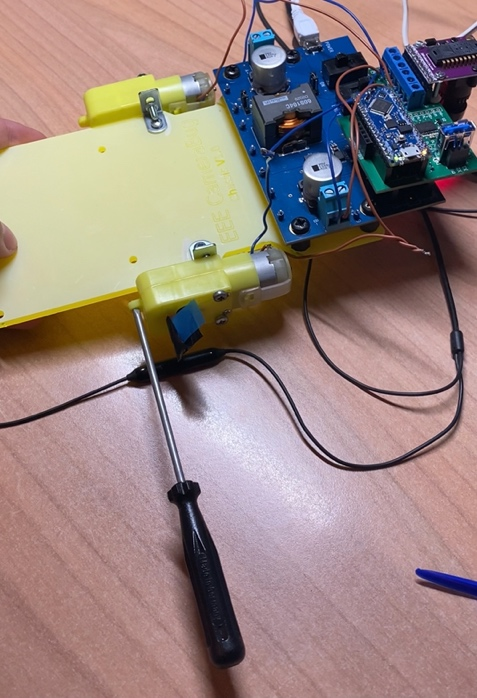
\includegraphics[width=2.16in,height=3.15in]{./media/image1.jpeg}
		\caption{Equipment Setup for Measuring RPM}
		\label{figDuring_the_process_of_recording}
	\end{Center}
\end{figure}


%%%%%%%%%%%%%%%%%%%% Figure/Image No: 2 Ends here %%%%%%%%%%%%%%%%%%%%

In the following table some basic specifications have been measured:


%%%%%%%%%%%%%%%%%%%% Table No: 1 starts here %%%%%%%%%%%%%%%%%%%%


\begin{table}[H]
 			\centering
\begin{tabular}{p{2.93in}p{2.93in}}
\hline
%row no:1
\multicolumn{1}{|p{2.93in}}{\Centering \textbf{\textit{Input}}} & 
\multicolumn{1}{|p{2.93in}|}{\Centering \textbf{\textit{Output}}} \\
\hhline{--}
%row no:2
\multicolumn{1}{|p{2.93in}}{Voltage $ \approx $ 5V} & 
\multicolumn{1}{|p{2.93in}|}{Minimum Operating Voltage: 1.384V \par Maximum Arduino's Voltage for accurate conversion: 4.096V \par } \\
\hhline{--}
%row no:3
\multicolumn{1}{|p{2.93in}}{Minimum Current: 0.134A \par Maximum Current: 0.22A \par } & 
\multicolumn{1}{|p{2.93in}|}{Minimum Operating Current: 0.035A \par Maximum Arduino's Current for accurate conversion: 0.060A \par } \\
\hhline{--}

\end{tabular}
 \end{table}


%%%%%%%%%%%%%%%%%%%% Table No: 1 ends here %%%%%%%%%%%%%%%%%%%%

\textbf{Speed Levels}

One of the main goals was to make the user interface with the rover relatively 
simple and that is why the idea of introducing 5 speed levels came up. 
Specifically, the idea behind those 5 speed levels, is to avoid using km/h or 
mph because the range of km/h is really small (0.17km/h-0.62km/h) and the range 
for the mph is even smaller (0.11mph-0.38mph) so, it will confuse the user. Thus,
one way to simplify the speed range is to set 5 speed levels that can be 
understood easily and be user friendly as well. Additionally, it is more 
convenient and straightforward as it does not require further knowledge 
(voltages, RPM).

In order to find the true range of voltages the rover's limits needs to be found. 
The code that is responsible for the voltage range has a reference voltage of 
4.096V. The value 4.096, is the Arduino's upper threshold for accurate 
conversion. On the other hand, the buck SMPS can generate up to 4.8V 
( due to the power losses it cannot generate exactly 5V). If the Arduino's 
reference voltage is increased then if, for example, a 2.5V reference voltage 
is sent to the rover, it  would not ``generate'' 2.5V as an input for the 
DC motors. This happens because the Arduino can handle only up to 4.096V and 
if this value is exceeded then the conversion will not be accurate. On the other 
hand, the lower limit is 1.46V because everything beyond that will not have enough 
power to move the rover. To conclude, the voltage range is from 1.46V to 4.096V in 
order to have a movable and an accurate rover. So, that is why the speed levels 
are divided like that. Those 5 speed levels can easily be ``corresponded'' to a 
specific voltage, and a specific voltage can easily be ``corresponded'' to a 
specific velocity.  After the the RPMs were found then, they were converted to 
speed values by the following formula:

$$ v \left(\frac{km}{hr}\right) = r \times \frac{2\pi}{60} \times N \left( rpm \right) \times 3.6  $$
% \[  \]  \[ v \left( \frac{km}{h} \right) =r\ast\frac{2 \pi }{60}\astN \sleft( rpm \right) \ast3.6 \] 
where r is the radius of the wheel and is equal to 3.4cm and the number 3.6 is used to convert m/s to km/h. 



%%%%%%%%%%%%%%%%%%%% Table No: 2 starts here %%%%%%%%%%%%%%%%%%%%


\begin{table}[H]
 			\centering
\begin{tabular}{p{0.67in}p{0.57in}p{0.62in}p{0.58in}p{0.78in}p{0.47in}p{0.47in}p{0.5in}}
\hline
%row no:1 
\multicolumn{1}{|p{0.67in}}{Speed Level} & 
\multicolumn{1}{|p{0.57in}}{RPM} & 
\multicolumn{1}{|p{0.62in}}{km/h} & 
\multicolumn{1}{|p{0.58in}}{mph} & 
\multicolumn{1}{|p{0.78in}}{Output Voltage(v)} & 
\multicolumn{1}{|p{0.47in}}{Input Voltage (V)} & 
\multicolumn{1}{|p{0.47in}}{Input Current (A)} & 
\multicolumn{1}{|p{0.5in}|}{Pin(W)} \\
\hhline{--------}
%row no:2
\multicolumn{1}{|p{0.67in}}{\textbf{Very fast }} & 
\multicolumn{1}{|p{0.57in}}{48.58 } & 
\multicolumn{1}{|p{0.62in}}{0.6227 } & 
\multicolumn{1}{|p{0.58in}}{0.3869 } & 
\multicolumn{1}{|p{0.78in}}{4.05} & 
\multicolumn{1}{|p{0.47in}}{4.95} & 
\multicolumn{1}{|p{0.47in}}{0.216} & 
\multicolumn{1}{|p{0.5in}|}{1.0692} \\
\hhline{--------}
%row no:3
\multicolumn{1}{|p{0.67in}}{\textbf{Fast}} & 
\multicolumn{1}{|p{0.57in}}{41.27 } & 
\multicolumn{1}{|p{0.62in}}{0.5289 } & 
\multicolumn{1}{|p{0.58in}}{0.3287 } & 
\multicolumn{1}{|p{0.78in}}{3.4} & 
\multicolumn{1}{|p{0.47in}}{4.96} & 
\multicolumn{1}{|p{0.47in}}{0.192} & 
\multicolumn{1}{|p{0.5in}|}{0.95232} \\
\hhline{--------}
%row no:4
\multicolumn{1}{|p{0.67in}}{\textbf{Regular}} & 
\multicolumn{1}{|p{0.57in}}{32.38 } & 
\multicolumn{1}{|p{0.62in}}{0.4150 } & 
\multicolumn{1}{|p{0.58in}}{0.2579 } & 
\multicolumn{1}{|p{0.78in}}{2.75} & 
\multicolumn{1}{|p{0.47in}}{4.97} & 
\multicolumn{1}{|p{0.47in}}{0.162} & 
\multicolumn{1}{|p{0.5in}|}{0.80514} \\
\hhline{--------}
%row no:5
\multicolumn{1}{|p{0.67in}}{\textbf{Slow}} & 
\multicolumn{1}{|p{0.57in}}{23.92 } & 
\multicolumn{1}{|p{0.62in}}{0.3066 } & 
\multicolumn{1}{|p{0.58in}}{0.1905 } & 
\multicolumn{1}{|p{0.78in}}{2.1} & 
\multicolumn{1}{|p{0.47in}}{4.98} & 
\multicolumn{1}{|p{0.47in}}{0.152} & 
\multicolumn{1}{|p{0.5in}|}{0.75696} \\
\hhline{--------}
%row no:6
\multicolumn{1}{|p{0.67in}}{\textbf{Very Slow}} & 
\multicolumn{1}{|p{0.57in}}{13.89 } & 
\multicolumn{1}{|p{0.62in}}{0.1780 } & 
\multicolumn{1}{|p{0.58in}}{0.1106 } & 
\multicolumn{1}{|p{0.78in}}{1.46} & 
\multicolumn{1}{|p{0.47in}}{4.99} & 
\multicolumn{1}{|p{0.47in}}{0.134} & 
\multicolumn{1}{|p{0.5in}|}{0.66866} \\
\hhline{--------}

\end{tabular}
 \end{table}


%%%%%%%%%%%%%%%%%%%% Table No: 2 ends here %%%%%%%%%%%%%%%%%%%%



One interesting observation is that the relationship between the voltage and the 
RPM is almost linear. This is confirmed in Figure \ref{graph: Output Voltage vs RPM}


 %%%%%%%%%%%%%%%%%%%  %  iGraph 1%%%%%%%%%%%%%%%%%%%%%%

 \begin{figure}[H]
    \centering
      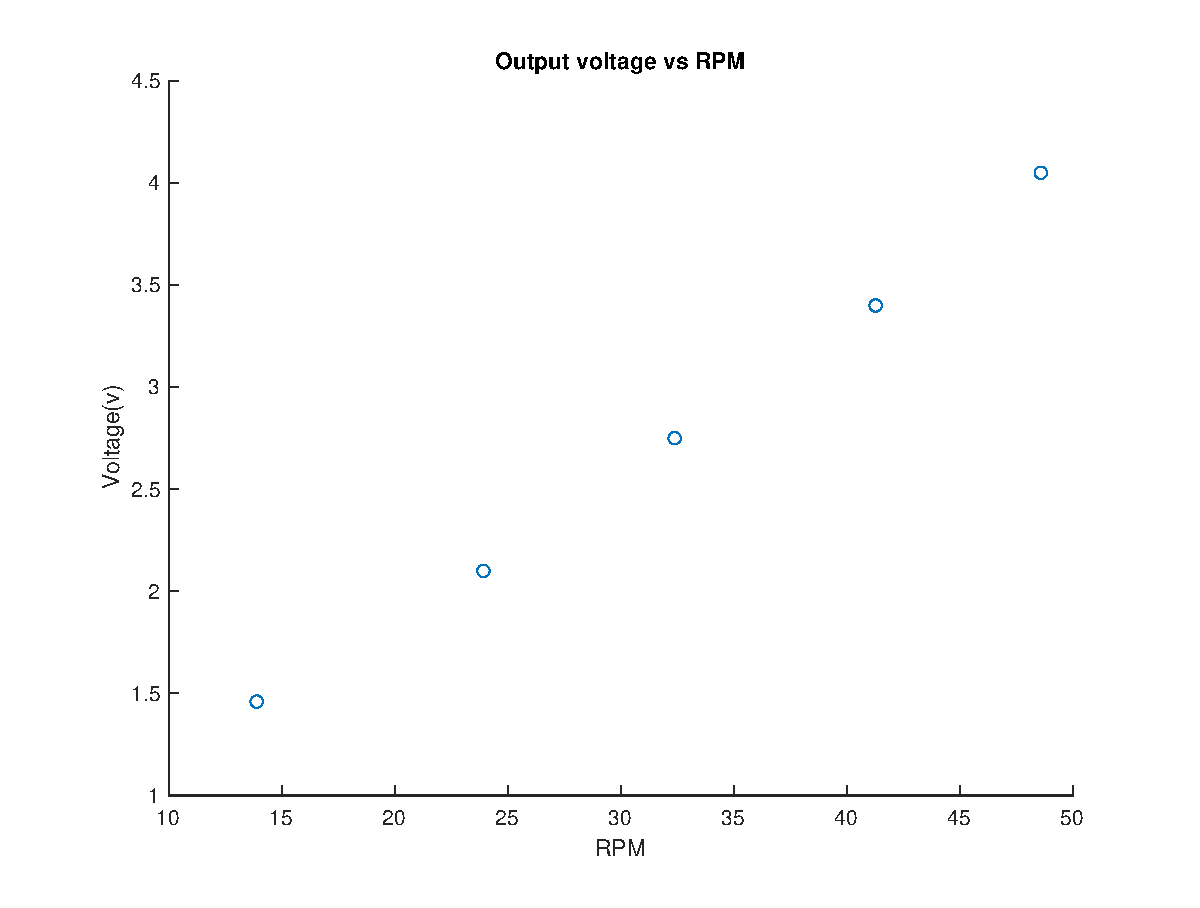
\includegraphics[scale=0.4]{./media/voltagevsrpm.eps}
   \caption{Output Voltage vs RPM}
   \label{graph: Output Voltage vs RPM}
    %\begin{minipage}{.7\textwidth}
      %\centering
      %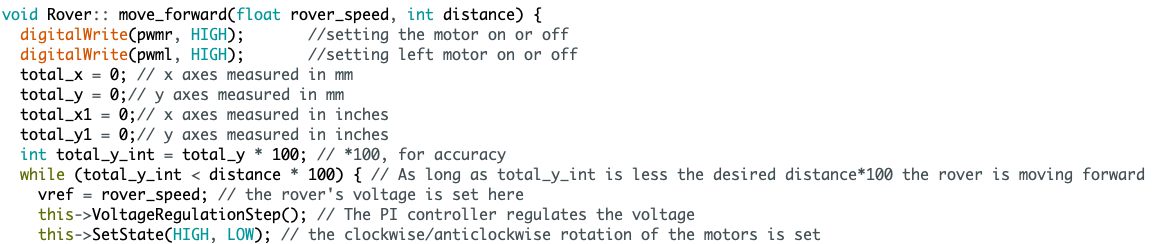
\includegraphics[scale=0.25]{./media/forward.png}
		%\caption{Forward Command Code}
      %\label{fig:Forward Command Code}
    %\end{minipage}
\end{figure}

%\begin{figure}
 %  \centering
  % 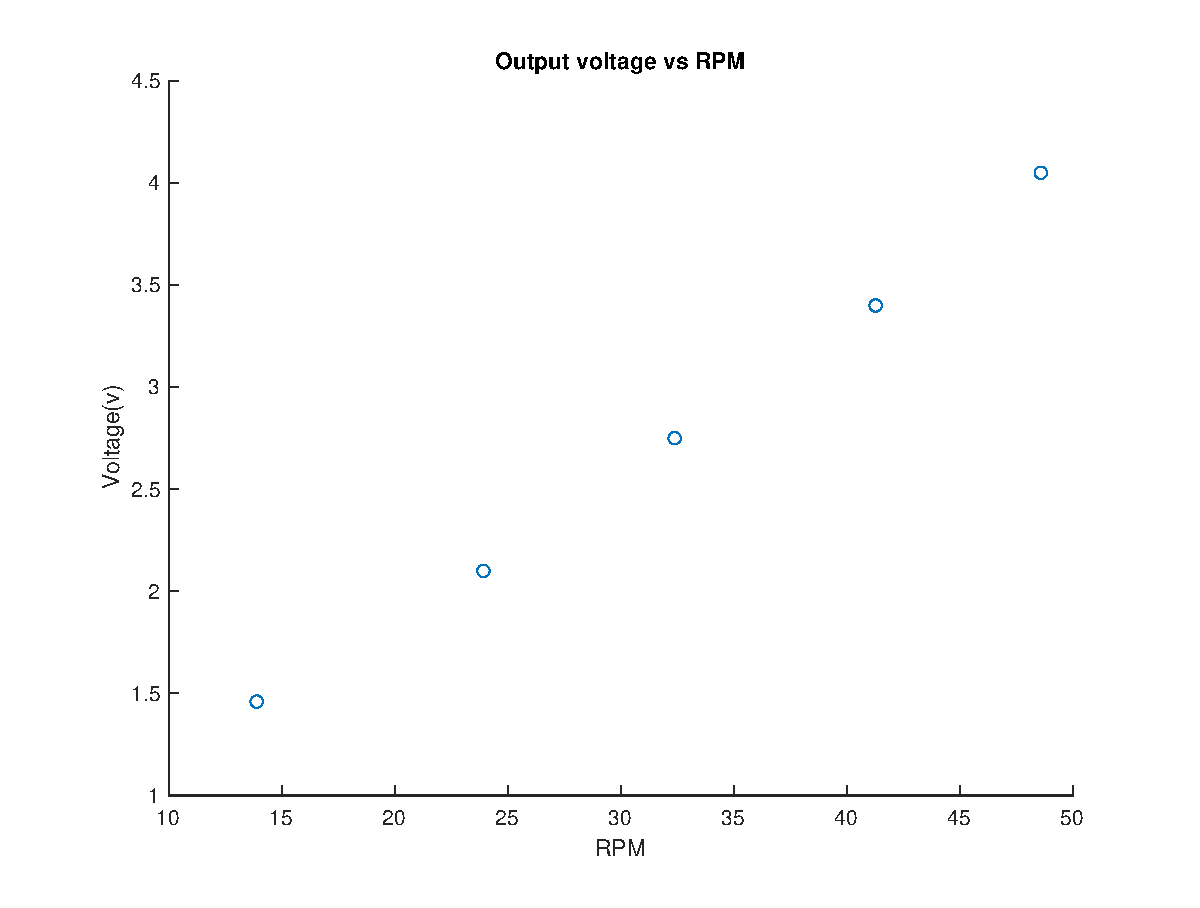
\includegraphics[scale=0.5]{./media/voltagevsrpm.eps}
   %\caption{Output Voltage vs RPM}
   %\label{graph: Output Voltage vs RPM}
%\end{figure}



%%%%%%%%%%%%%%%%Graph2 ends here%%%%%%%%%%%%%%%%%%%%%%%%
\paragraph*{Commands}


After finding the specifications the next step was to make a movable rover. 
Initially, one crucial task to do was to simplify and ``connect''  the two 
sample codes. To do that, there was a need for the use of an object oriented 
approach which would make it feasible to combine functions of the two sample 
codes into two different objects. In this case classes were used to implement 
a rover object and an optical flow sensor object. This allows to use the 
complicated code of the optical flow sensor in a simple way inside the rover 
functions.After, making the code simple and creating classes that would make 
the testing straightforward, 2 major changes were made to the code. Firstly, 
even though the control knob was really helpful to measure some key data, 
for the project it was needed to be able to set output voltages independently 
of the control knob and that is why it was not used. Specifically, the voltage 
of the DC motors is now being controlled by the user with those 5 speed levels. 
Secondly, the optical flow sensor was connected directly to the code that is 
responsible for the movement of the rover. In other words, the rover was able 
to move backward and forward by just setting inside a while loop the desired 
distance and comparing it with the measurements of the optical flow sensor. 
For example, the desired distance is 20cm, the rover will be moving forward 
or backward until the measurements read from the optical flow sensor for the 
y axes are approximately equal to 20cm.

\begin{figure}[H]
	\begin{Center}
		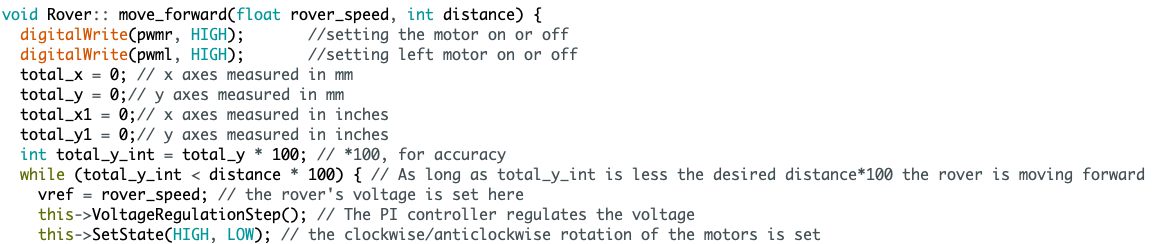
\includegraphics[scale=0.3]{./media/forward.png}
		\caption{Forward Command Code}
	\end{Center}
\end{figure}


Additionally, to make the rover rotate clockwise and anticlockwise the 
following process was implemented: Assuming that the centre of the rover 
(the centre of the imaginary axes that connects the two DC motors) is not 
rotating and it remains in the same position while the main body is rotating, 
then it can concluded that the rover is tracing an arc. The imaginary arc with 
the body of the rover is forming a circular sector. The radius of the imaginary 
circular sector is the length from the centre of the optical flow sensor to the 
centre of the imaginary axes that connects the DC motors. The mathematical 
formula is given as follows  \( \textbf{arc length}= \theta r \), where  \(\theta\)   is 
the angle in radians and \(r\) is the radius. So, to implement this, as seen in Figure \ref{fig: Clockwise Command Code} a while loop 
in the code was implemented to make the rover to rotate as long as the traced 
path of the optical flow sensor is less than the arc length needed to be traced 
to cover a specific angle. For example, if the desired angle is 90\degree \   
or  \( \frac{ \pi }{2} \)  the rover will be rotating until the measured path 
of the optical flow sensor (the x value that is being measured from the optical 
flow sensor) is equal to the angle times the radius. The radius is approximately 
168 mm but in the code it has been adjusted in order the rotation command to be 
accurate.

%\begin{figure}[H]
	%\begin{Center}
		%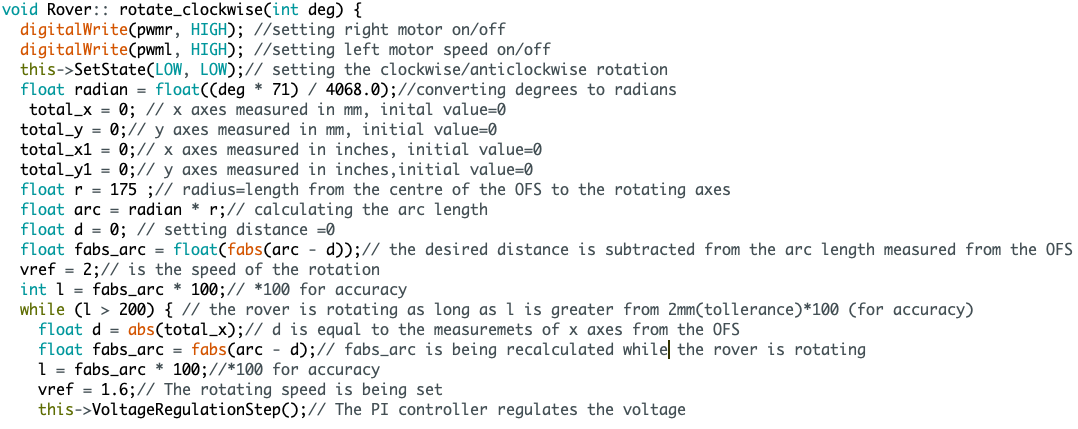
\includegraphics[scale=0.3]{./media/clockwise.png}
		%\caption{Clockwise Command Code}
	%\end{Center}
%\end{figure}

\begin{figure}[H]
    \centering
    \begin{minipage}{.7\textwidth}
      \centering
      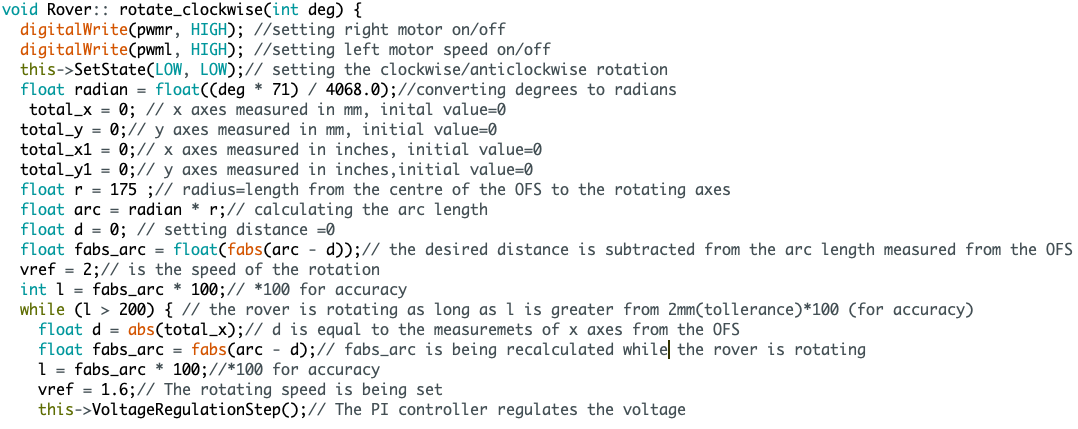
\includegraphics[scale=0.3]{./media/clockwise.png}
      \caption{Clockwise Command Code}
      \label{fig: Clockwise Command Code}
    \end{minipage}%
%%%%%%%%%%%%%%%%%%%% Figure/Image No: 3 starts here %%%%%%%%%%%%%%%%%%%%
    \begin{minipage}{.3\textwidth}
      \centering
      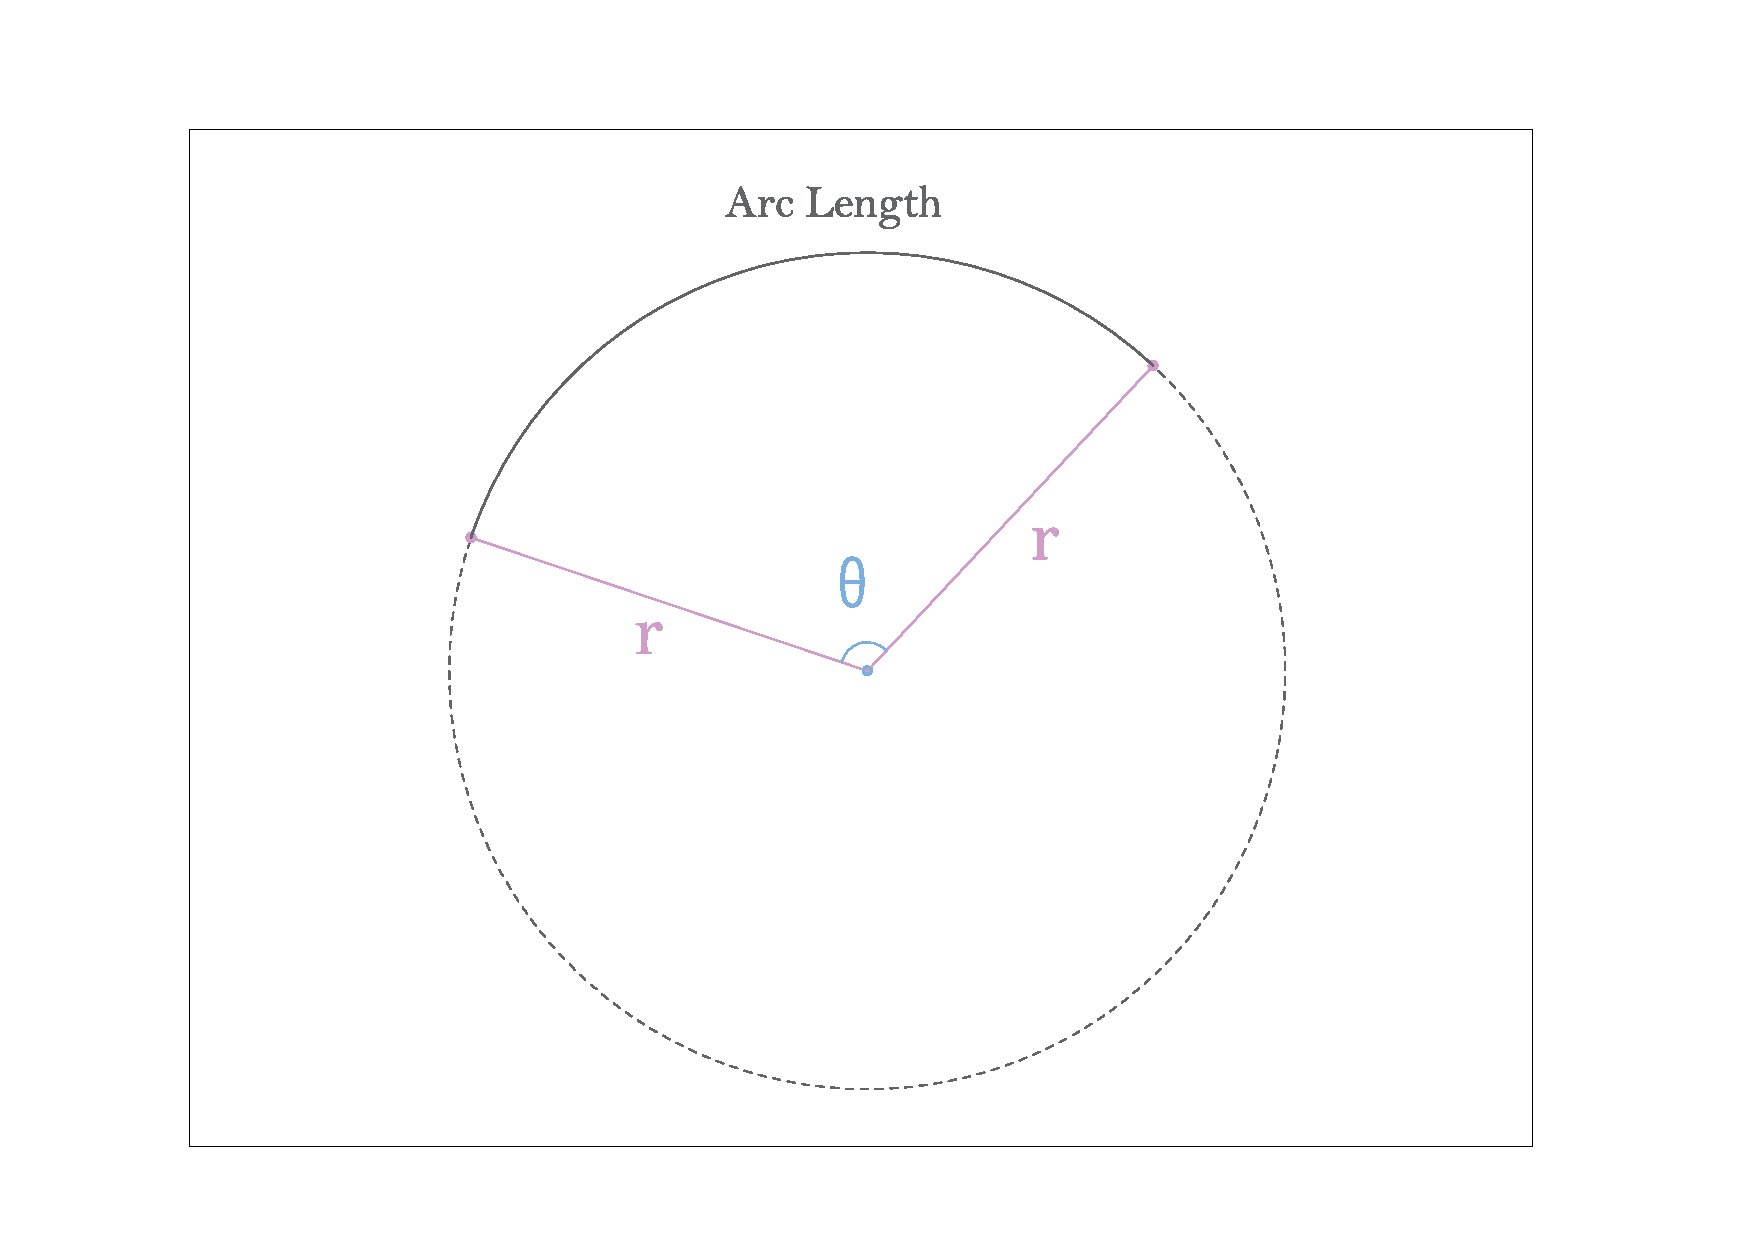
\includegraphics[scale = 0.2]{./media/image3.pdf}
      \caption{The arc that the \\ optical flow sensor is tracing}
      \label{fig: Optical Flow Sensor Arc}
    \end{minipage}
\end{figure}

   
%\begin{figure}[H]
%\begin{center}
%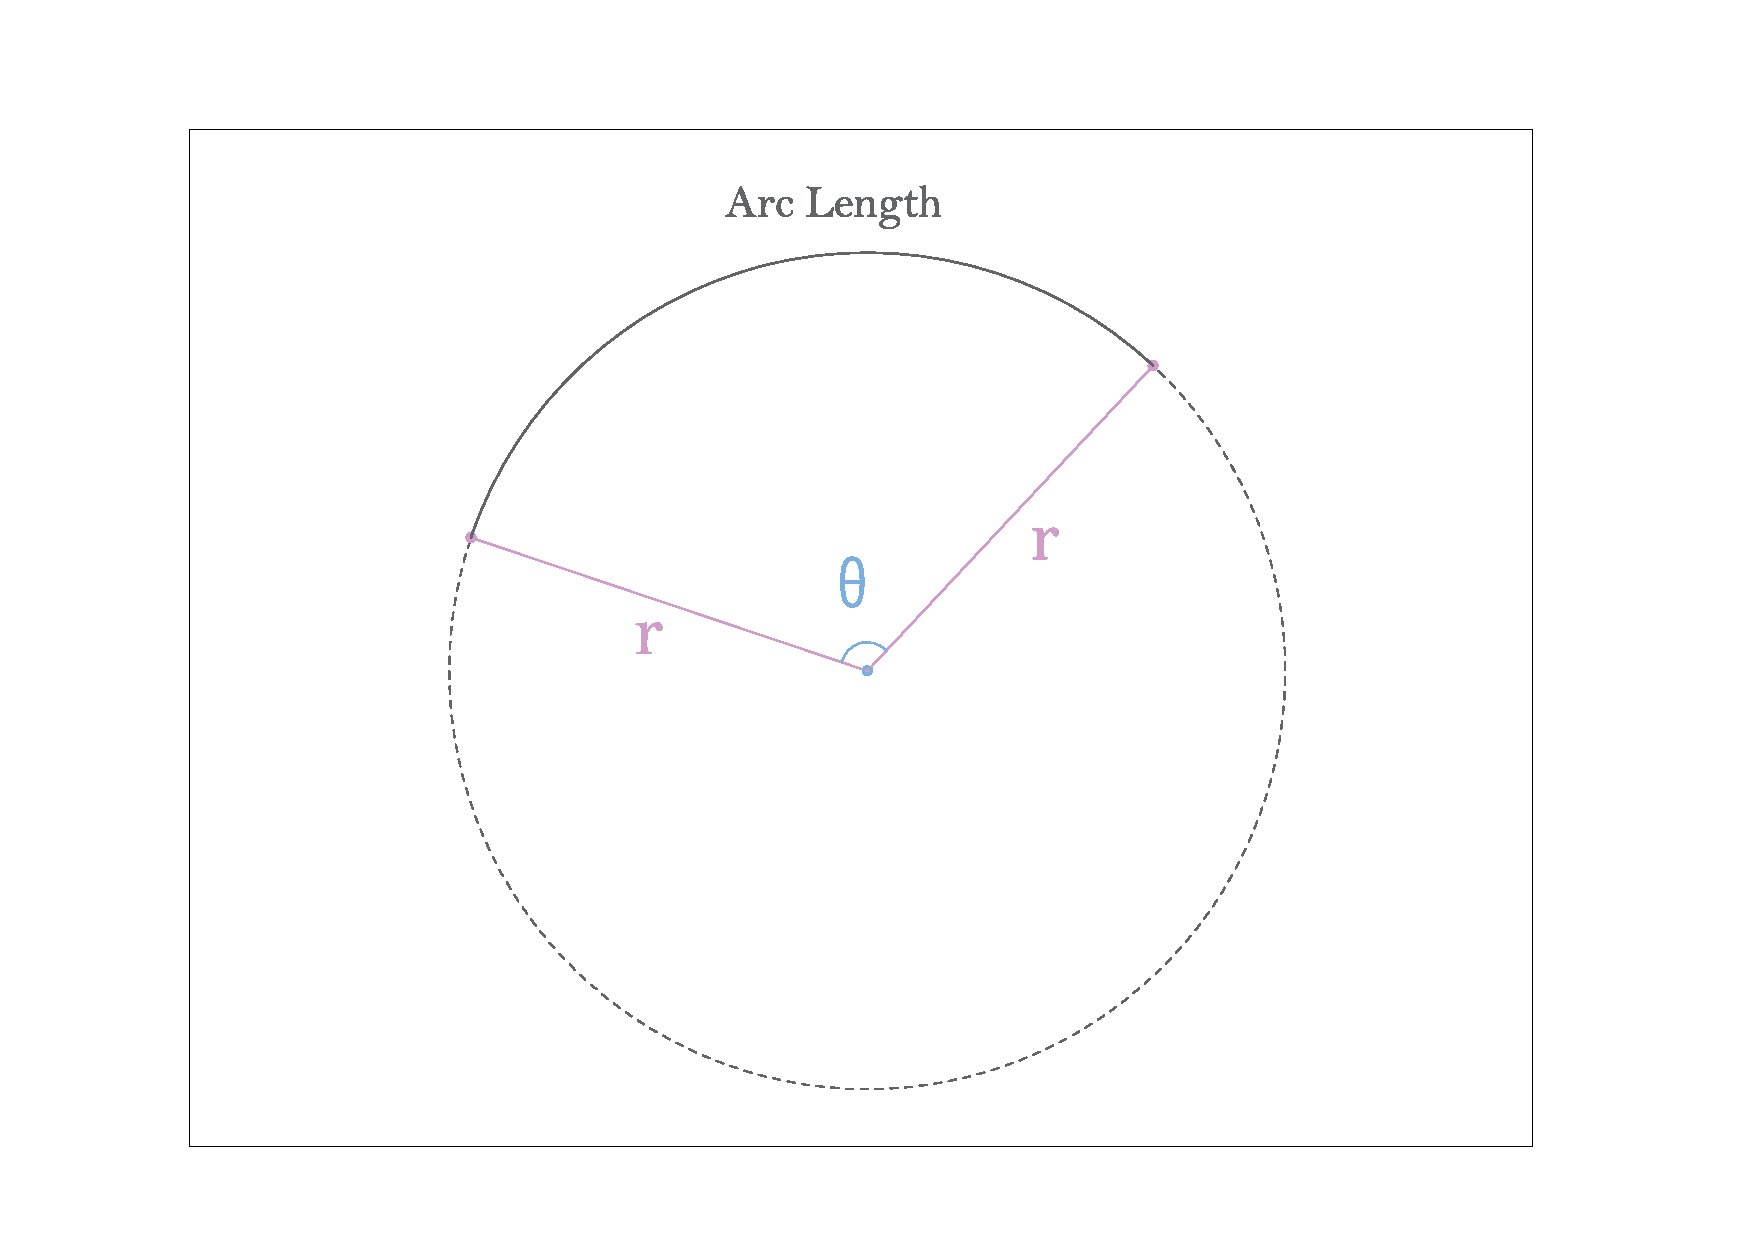
\includegraphics[width=3in,height=3in]{./media/image3.pdf}
%\caption{The arc that the optical flow sensor is tracing }
		%\end{center}
%\end{figure}

%%%%%%%%%%%%%%%%%%%% Figure/Image No: 3 Ends here %%%%%%%%%%%%%%%%%%%%




\paragraph*{Controller}

The voltage controller had some pre-set values. Using the trial and error method, 
initially,  only one of the three variables of the PID controller was changed at 
a time while the others remained set. Regarding the derivative controller, it 
made the system unstable because it made it oscillating and inaccurate. So, 
the best choice was to set the Derivative controller equal to 0. Additionally, 
the combination of changes in the PI controller values decreased the settling 
time, the rise time, the overshoot and the steady state error. As it can be seen 
in the graph bellow, the difference between the initial and the final PID values 
is significant. The overshoot has been eliminated, the rise and the settling 
time have been improved dramatically and the steady state error has an acceptable 
value. Furthermore, it is worth mentioning that if the ratio  \( \frac{ki}{kp} \)  
is great enough (larger than 8) then the response of the system becomes almost 
perfect.
To conclude, by using only a PI controller and by setting P=2.6 and I=27 the 
rover has a stable driving system that does not take a lot of time to stabilise 
its reference voltage (in other words, its reference speed), and most importantly, 
it does not overshoot and oscillate before it takes its reference value. 
These findings can be confirmed by the graph shown in Figure ~\ref{graph:Initial vs Final PI controller}

%%%%%%%%%%%%%%%%%%%% Figure/Image No: 4 starts here %%%%%%%%%%%%%%%%%%%%

\begin{comment}
\begin{figure}[H]
   \centering
   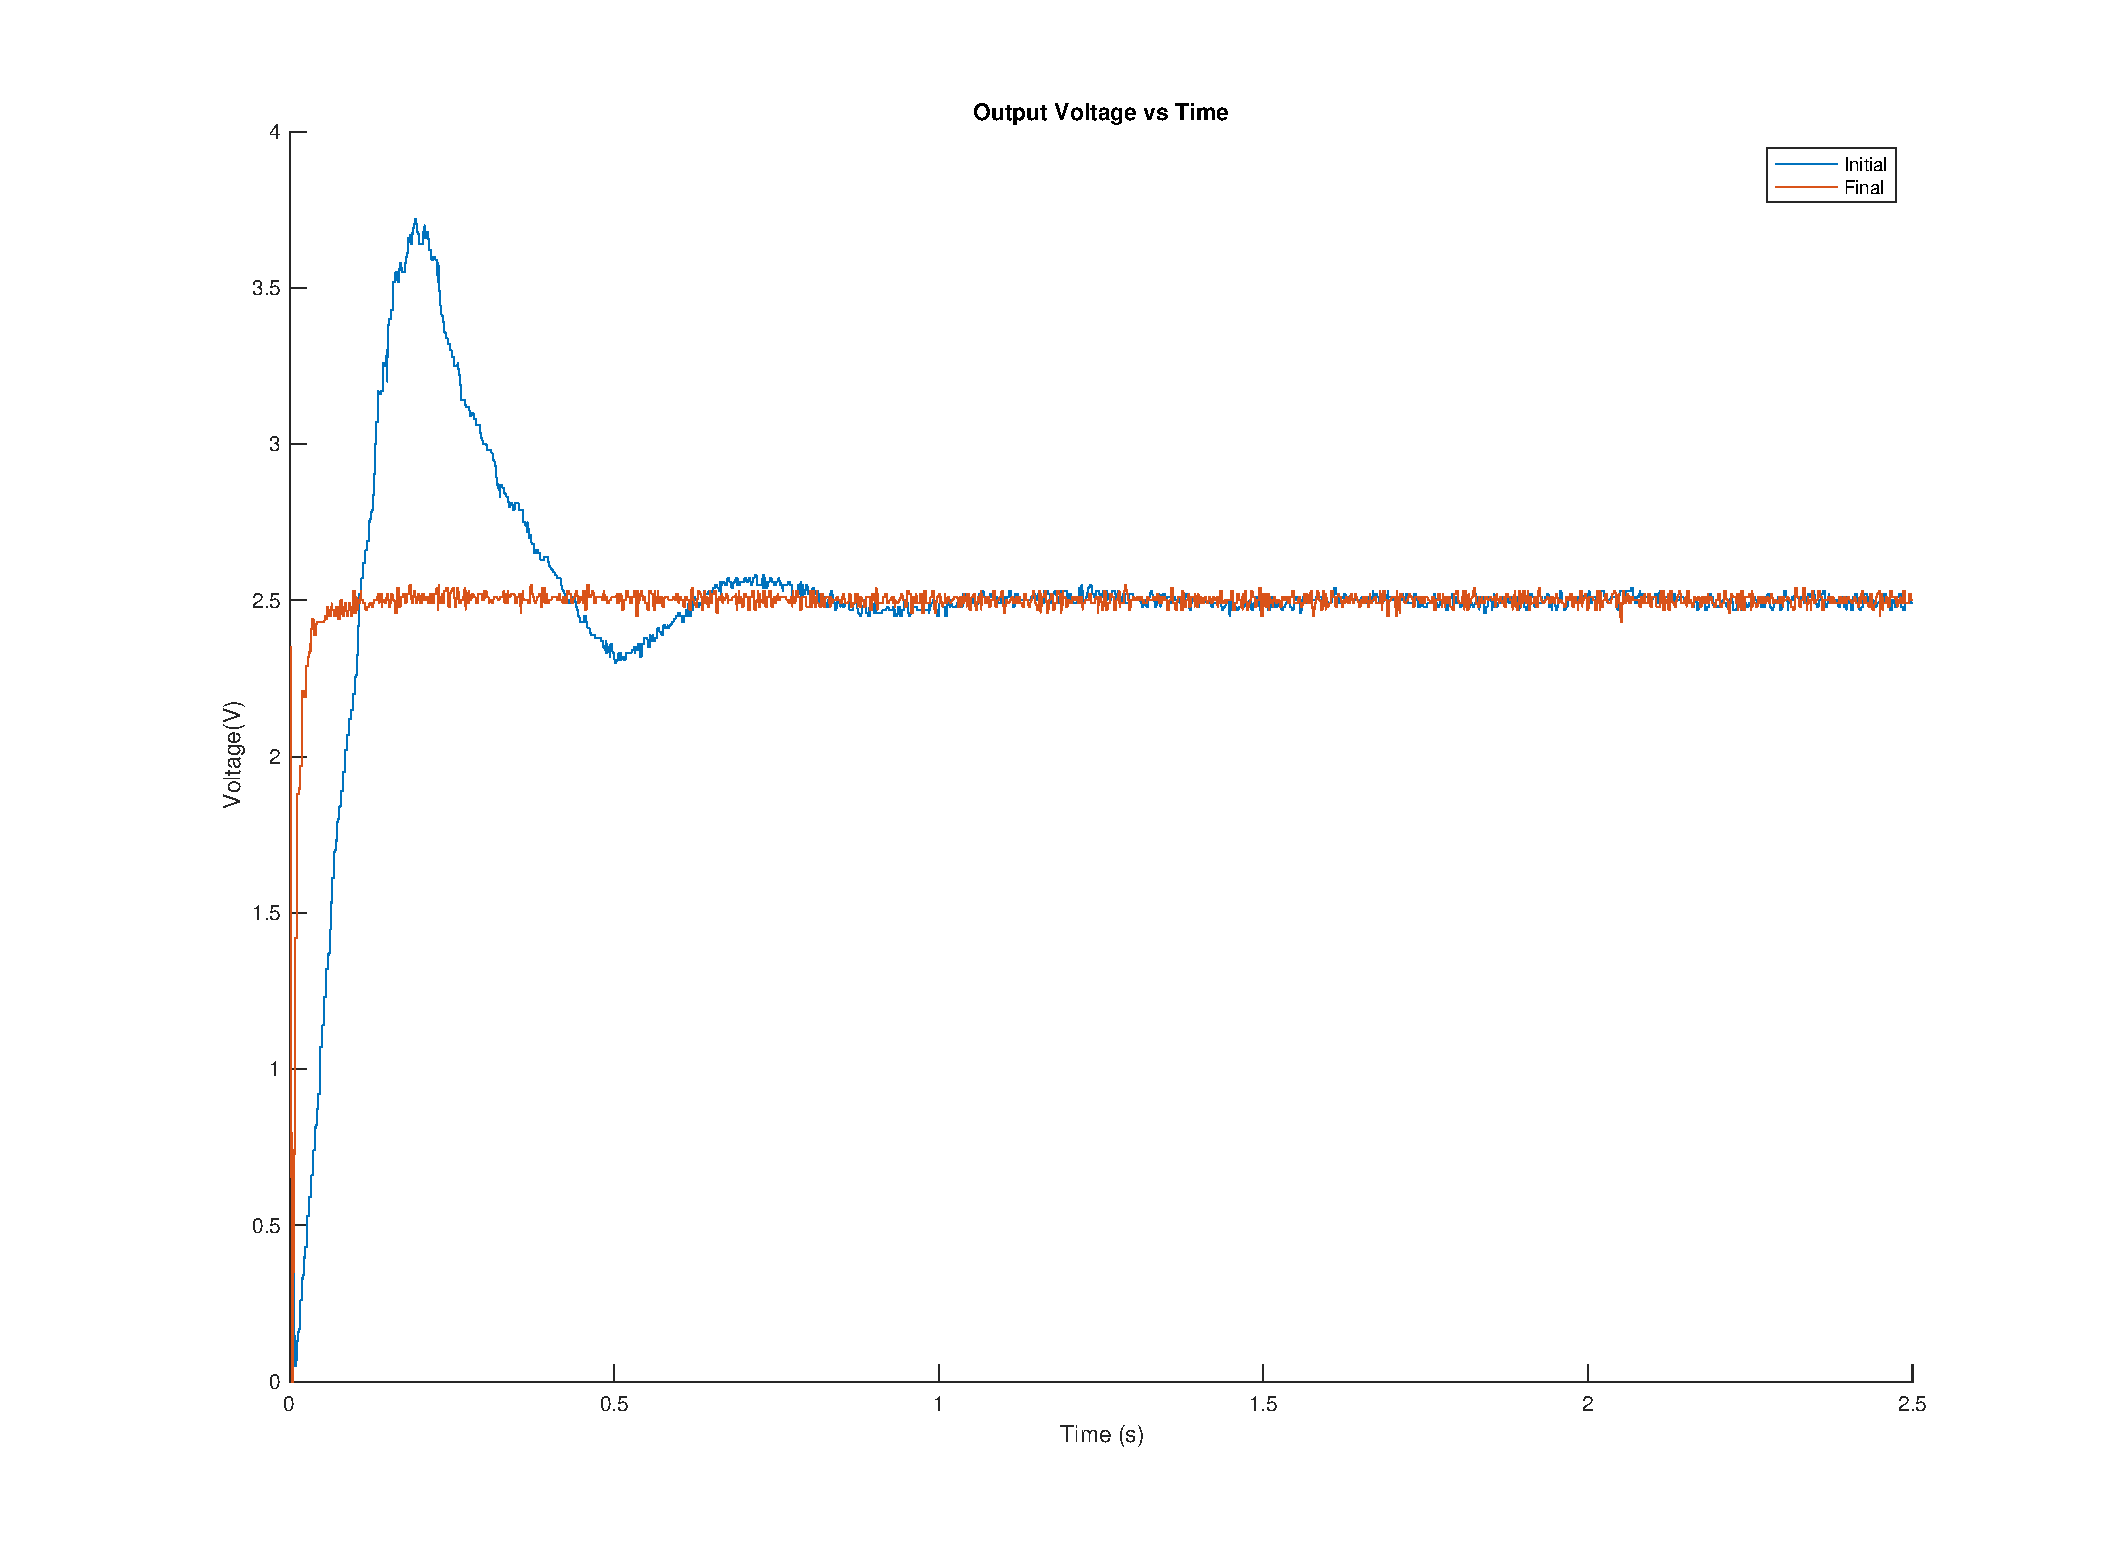
\includegraphics[scale=0.3]{./media/initialvsfinal.eps}
   \caption{Initial vs Final PI controller}
   \label{graph:Initial vs Final PI controller}
\end{figure}
\end{comment}

\begin{figure}[H]
    \centering
    \begin{minipage}{.4\textwidth}
        \centering
        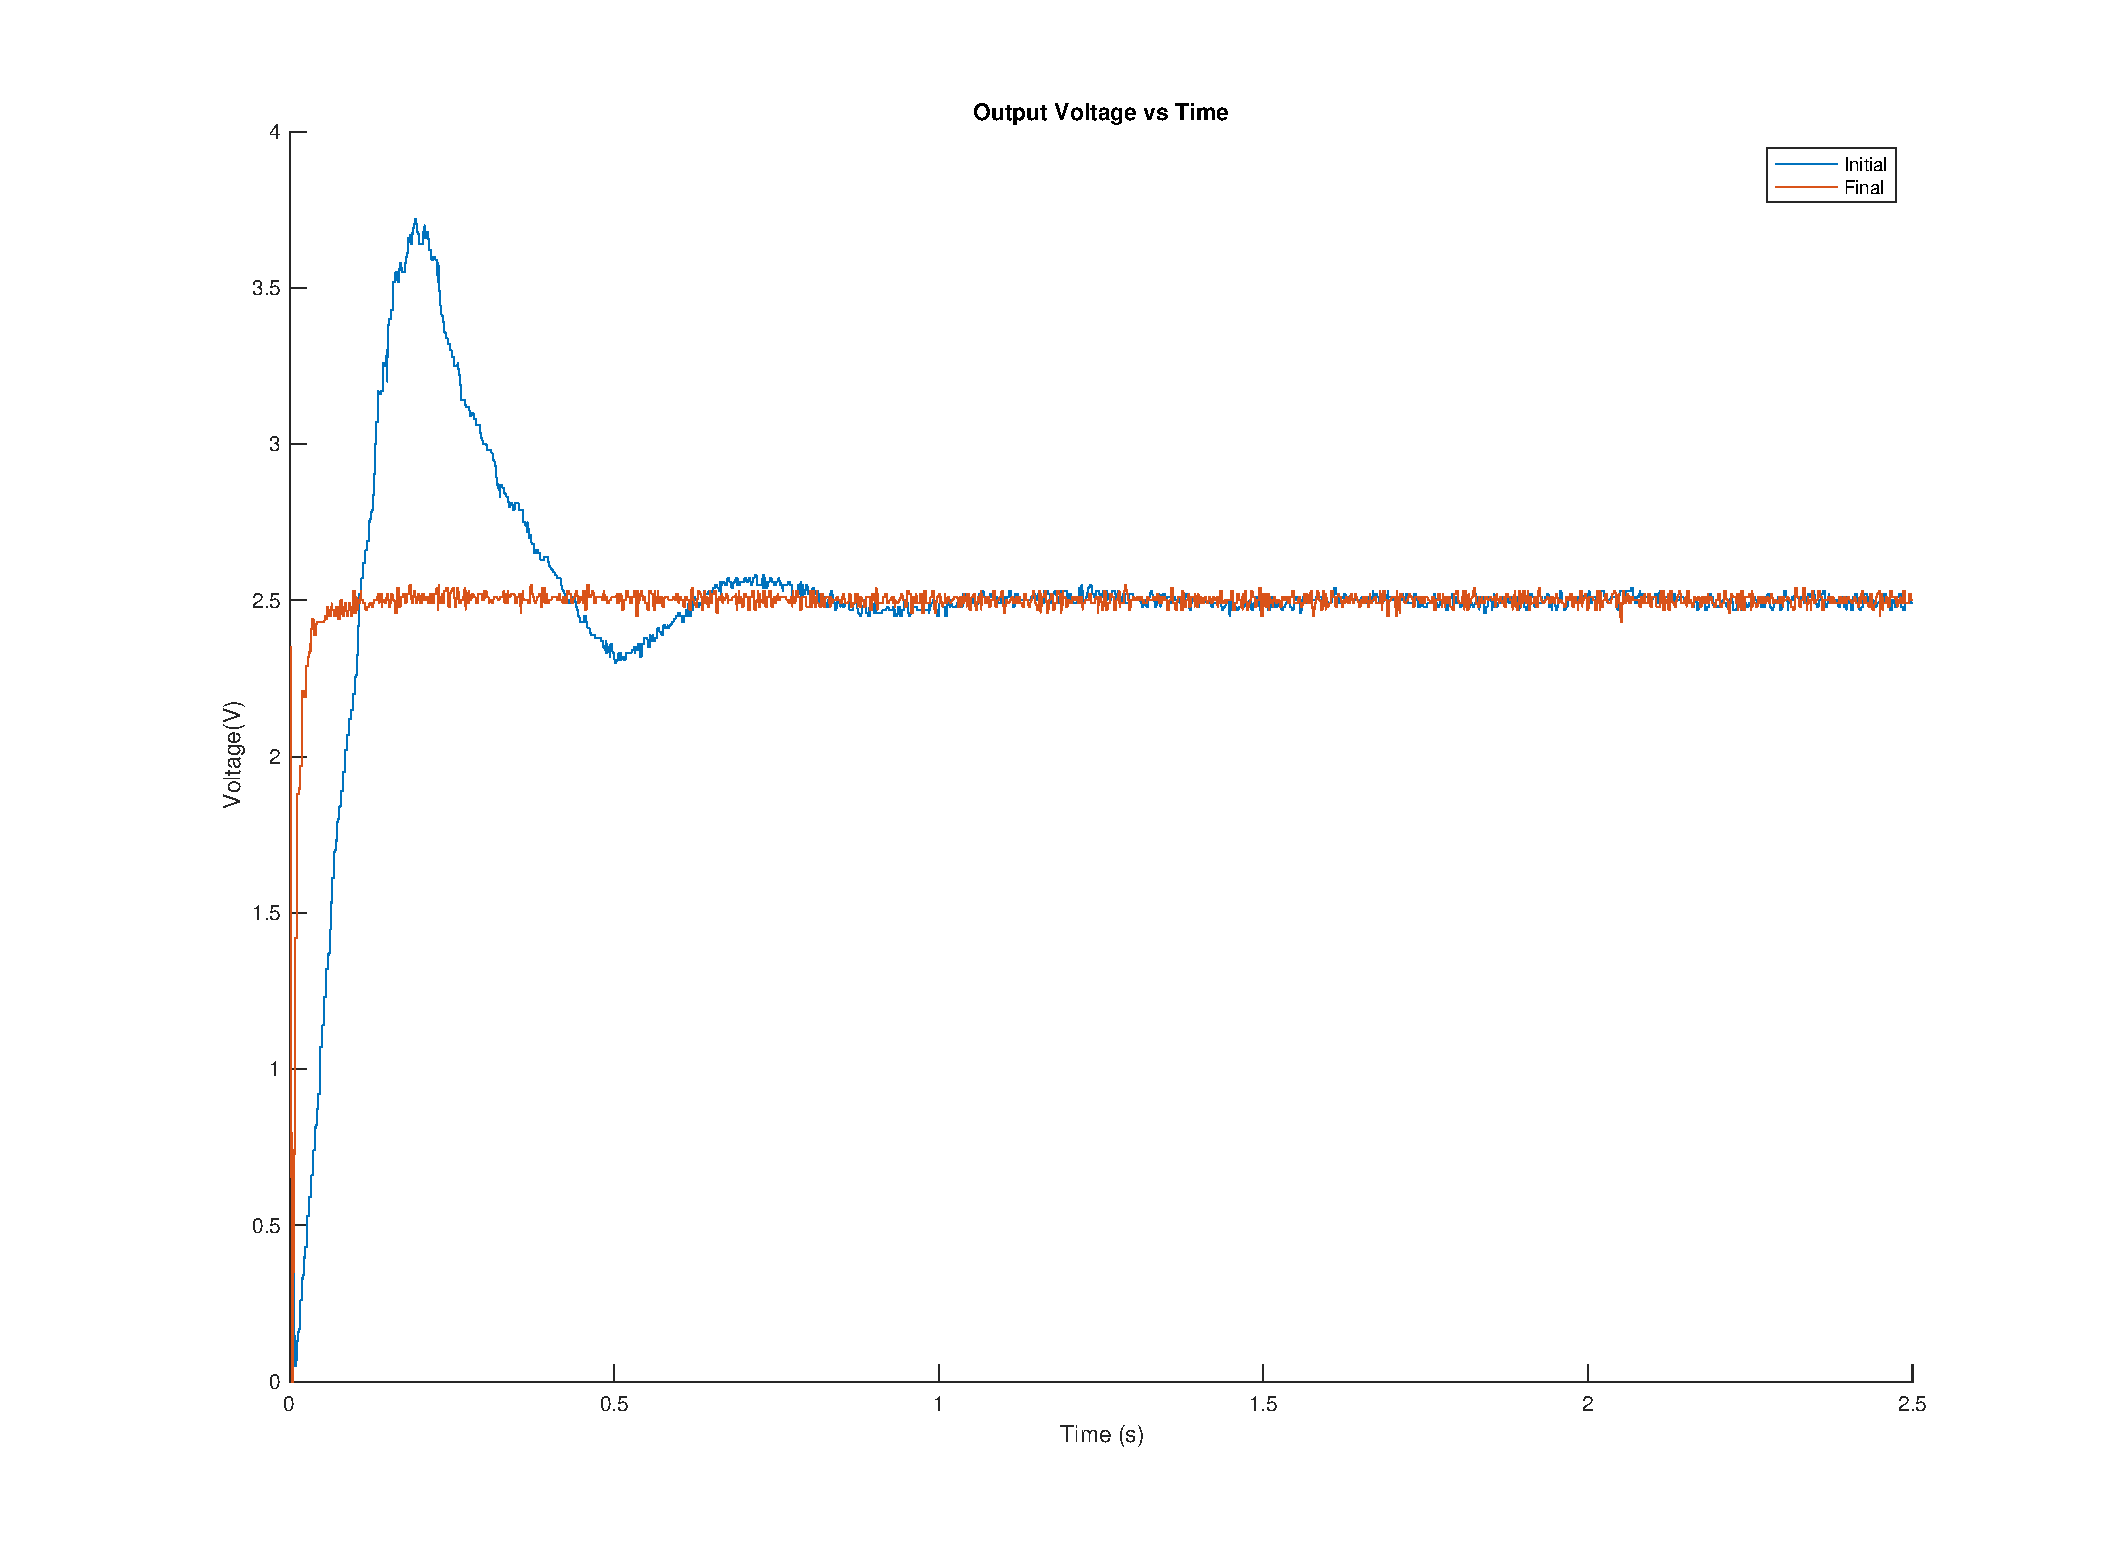
\includegraphics[scale=0.178]{./media/initialvsfinal.eps}
        \caption{Initial vs Final PI controller}
        \label{graph:Initial vs Final PI controller}
    \end{minipage}%
    \begin{minipage}{.6\textwidth}
        \centering
        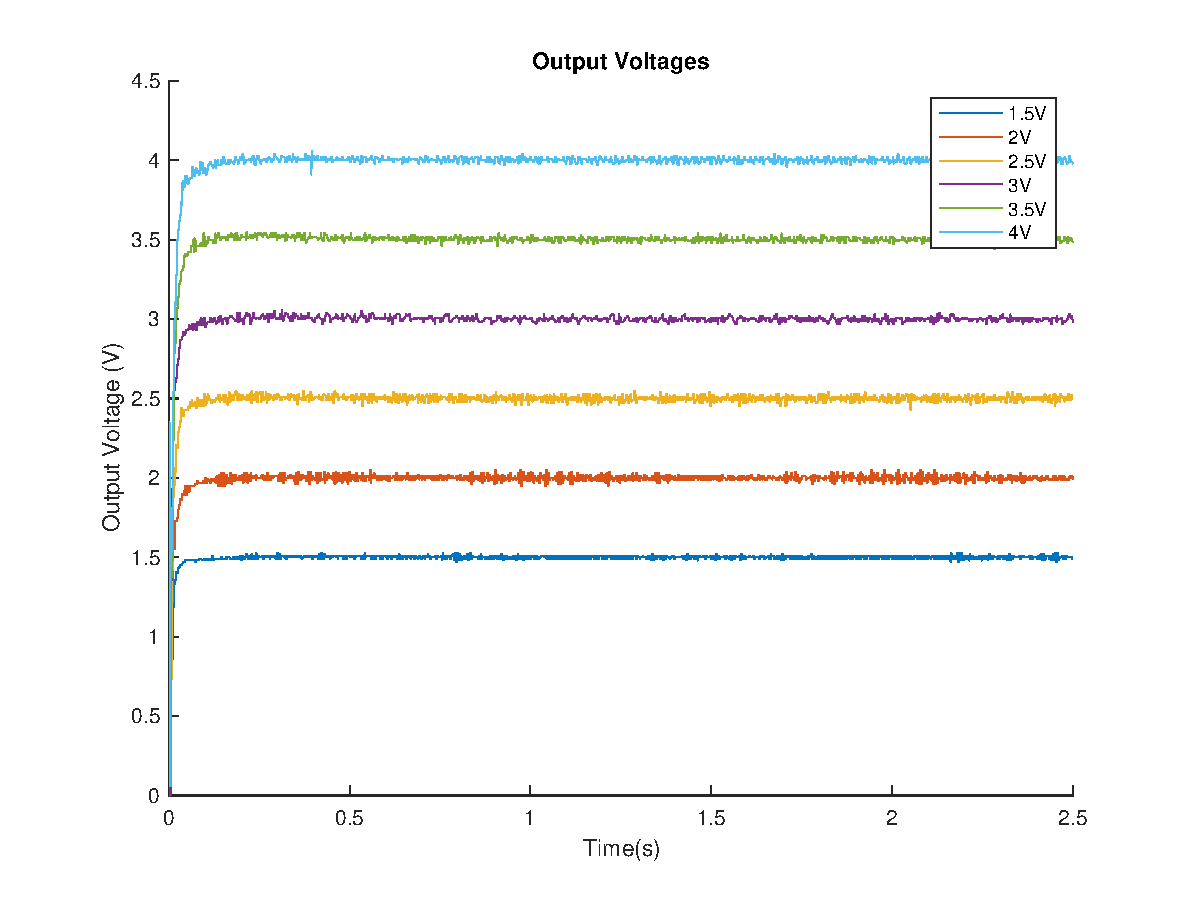
\includegraphics[scale=0.35]{./media/allvoltages.eps}
        \caption{Output Voltages for all Reference Voltages }
        \label{graph:Output Voltages}
    \end{minipage}
\end{figure}

The difference in the system's response is obvious as the system with the final PI values almost instantly reaches its reference value.
The table below is showing the performance of the two PI controllers:


%%%%%%%%%%%%%%%%%%%% Figure/Image No: 4 Ends here %%%%%%%%%%%%%%%%%%%%

%%%%%%%%%%%%%%%%%%%% Table No: 3 starts here %%%%%%%%%%%%%%%%%%%%


\begin{table}[H]
 			\centering
\begin{tabular}{p{0.83in}p{0.99in}p{0.84in}p{0.84in}p{0.84in}}
\hline
%row no:1
\multicolumn{1}{|p{0.83in}}{} & 
\multicolumn{1}{|p{0.99in}}{Overshoot($\%$)} & 
\multicolumn{1}{|p{0.84in}}{Rise time(s)} & 
\multicolumn{1}{|p{0.84in}}{Settling time(s)} & 
\multicolumn{1}{|p{0.84in}|}{Steady State Error($\%$ )} \\
\hhline{-----}
%row no:2
\multicolumn{1}{|p{0.83in}}{Initial} & 
\multicolumn{1}{|p{0.99in}}{48} & 
\multicolumn{1}{|p{0.84in}}{0.143} & 
\multicolumn{1}{|p{0.84in}}{1.25} & 
\multicolumn{1}{|p{0.84in}|}{1.8} \\
\hhline{-----}
%row no:3
\multicolumn{1}{|p{0.83in}}{Final} & 
\multicolumn{1}{|p{0.99in}}{-} & 
\multicolumn{1}{|p{0.84in}}{0.0136} & 
\multicolumn{1}{|p{0.84in}}{0.12} & 
\multicolumn{1}{|p{0.84in}|}{1.6} \\
\hhline{-----}

\end{tabular}
 \end{table}


%%%%%%%%%%%%%%%%%%%% Table No: 3 ends here %%%%%%%%%%%%%%%%%%%%




As it can be seen in Figure \ref{graph:Initial vs Final PI controller}, using the previous PI values the system 
responds perfectly for all the reference voltages. Also, in the table below are 
given the steady state error for every voltage value. It is really important 
that the system after it has reached its reference value, it does not fluctuate. 




%%%%%%%%%%%%%%%%%%%% Table No: 4 starts here %%%%%%%%%%%%%%%%%%%%


\begin{table}[H]
 			\centering
\begin{tabular}{p{0.73in}p{0.68in}p{0.68in}p{0.68in}p{0.68in}p{0.68in}p{0.69in}}
\hline
%row no:1
\multicolumn{1}{|p{0.80in}}{Voltages(V)} & 
\multicolumn{1}{|p{0.68in}}{1.5} & 
\multicolumn{1}{|p{0.68in}}{2} & 
\multicolumn{1}{|p{0.68in}}{2.5} & 
\multicolumn{1}{|p{0.68in}}{3} & 
\multicolumn{1}{|p{0.68in}}{3.5} & 
\multicolumn{1}{|p{0.69in}|}{4} \\
\hhline{-------}
%row no:2
\multicolumn{1}{|p{0.80in}}{Steady State Error} & %($\%$)
\multicolumn{1}{|p{0.68in}}{1.3} & 
\multicolumn{1}{|p{0.68in}}{2} & 
\multicolumn{1}{|p{0.68in}}{1.6} & 
\multicolumn{1}{|p{0.68in}}{1} & 
\multicolumn{1}{|p{0.68in}}{1} & 
\multicolumn{1}{|p{0.69in}|}{0.75} \\
\hhline{-------}

\end{tabular}
 \end{table}


%%%%%%%%%%%%%%%%%%%% Table No: 4 ends here %%%%%%%%%%%%%%%%%%%%




%%%%%%%%%%%%%%%%%%%% GRAPH No: 5 starts here %%%%%%%%%%%%%%%%%%%%
%\begin{center}
   %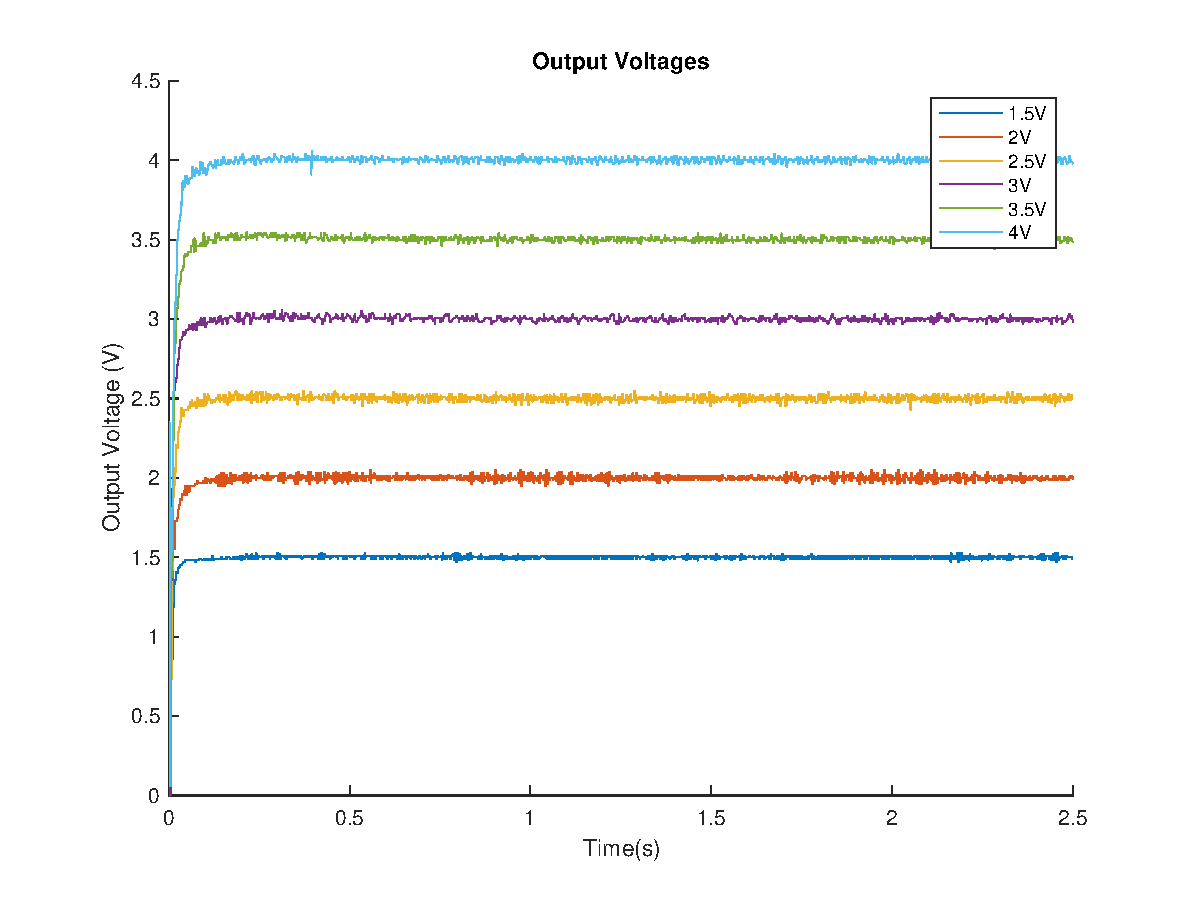
\includegraphics[scale=0.5]{./media/allvoltages.eps}
%\end{center}

\begin{comment}
\begin{figure}
    \centering
    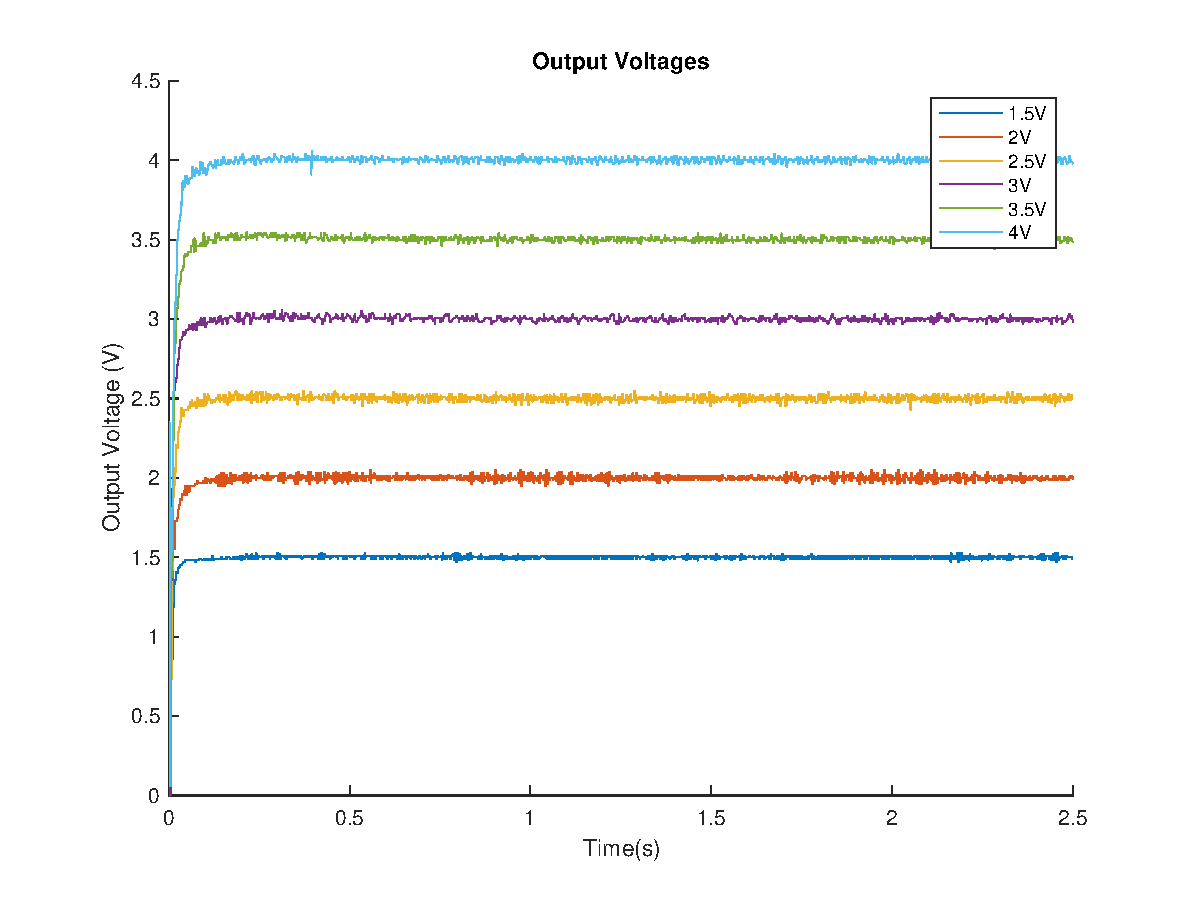
\includegraphics[scale=0.5]{./media/allvoltages.eps}
    \caption{Output Voltages for all Reference Voltages }
    \label{graph:Output Voltages}
 \end{figure}
\end{comment}



%%%%%%%%%%%%%%%%%%%% GRAPH No: 5 Ends here %%%%%%%%%%%%%%%%%%%%
Regarding the Current Controller, it was not tuned because the voltage controller
 interacts with it. Thus, after further testing, making changes to the PI current
  controller gains was not necessary. Finally, the current instantly takes the 
  desired value and it does not oscillate. 





\pagebreak
\subsection{Vision}

The purpose of the Vision module as aforementioned was to find different coloured
ping-pong balls and draw bounding boxes around them to find their estimated location, 
the desired outcome is shown in Figure \ref{fig:DesiredVisionResult}. The following 
section is organised in order of the video processing stream: first the raw data to 
RGB data, then the transformation to the HSV colour space, followed by the object 
detection, then finally the calculation for the estimated distance of each ball. 

\begin{figure}[H]
	\begin{Center}
		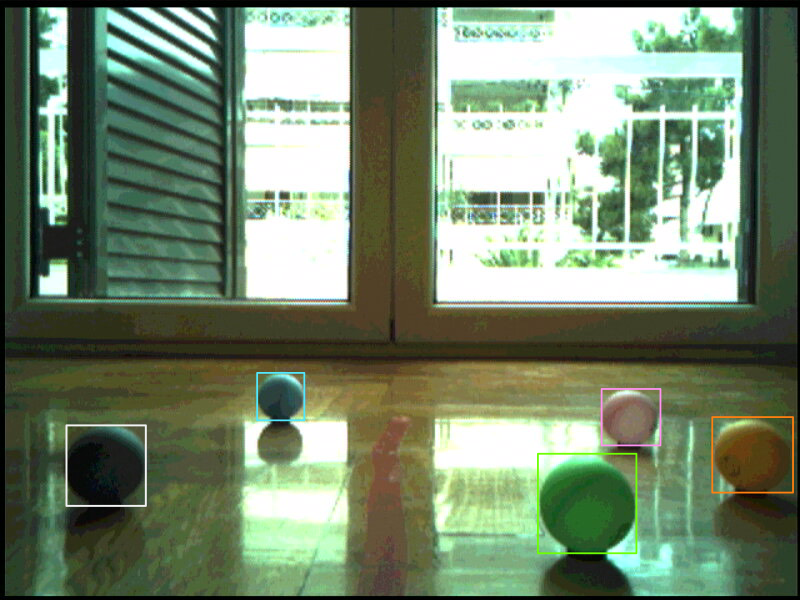
\includegraphics[scale = 0.5]{./images/AnnotatedBalls.png}
		\caption{Desired Outcome of Image Processing applied in Vision module }
		\label{fig:DesiredVisionResult}
	\end{Center}
\end{figure}



 

\subsubsection{Image Capture \& Processing Stream}

The image capture and buffering is based on a starter project provided
by Terasic Inc for the D8M Camera module that was modified by Dr Edward Stott 
\cite{EEE2Rover} and provided to us for this project. The system makes use of 
several IP components from the Intel Video and Image Processing Suite,
namely the Clocked Video Output and Frame Buffer Core. The system is compromised
of several modules, that take the raw data from the camera in Bayer filter form\cite{TerasicD8MWeb},
transform it into RGB video packets with a resolution of 640*480, buffer the frames to allow camera and output
to run at different frame rates, process the image data and convert the video 
data to serial data for output over VGA.\cite{EEE2Rover} As this system and its 
corresponding documentation is openly available, the implementation outside of 
the image processor will not be described in more depth, interested readers can 
consult the referenced repository and starter project for more information. 

\subsubsection{Image Pre-Processing Module - RGB to HSV Conversion} 


HSV is traditionally expressed as three values ranging between 0-360\degree\  
for hue, and two values between 0 and 1 for saturation and value.\cite{10.1145/965139.807361}
As floating point calculations in SystemVerilog are computationally expensive, 
and also introduce a layer of unnecessary complexity, the conversion was adjusted
to express all three values in terms of an 8 bit integer ranging from 0-255. The
algorithm for conversion from 8-bit RGB integers is presented mathematically:

\begin{multicols}{3}
    \noindent
    \begin{align*}
        M &= \max(R, G, B) \\ \\
        m &= \min(R, G, B) \\ \\
        C &= M-m 
    \end{align*}
    \begin{equation*}
        H = \begin{cases}
            M = R, & 0 + \frac{43 \times (G-B)}{C} \\
            M = G, & 85 + \frac{43 \times (B-R)}{C} \\
            M = B, & 171 + \frac{43 \times (R-G)}{C} \\
            M = 0, & 0 \\
            C = 0, & 0
        \end{cases} 
    \end{equation*}
    \begin{align*}
        S &= \begin{cases}
            M = 0, & 0 \\ C = 0, & 0 \\ \text{else} & \frac{255\times C}{V}
        \end{cases} & \\ \\
         V &= M  
    \end{align*}
\end{multicols}



Although the inclusion of a divide operation was undesirable as it does not 
translate well to hardware implementations, it was unavoidable with hue being 
obtained by dividing the difference of two components by the chroma value. This 
is a result of HSV being a non-linear transform from HSV. 

The YUV colour space was also considered as a option for conversion as it also
separates colour into 3 components - one for luma and two chrominance components.
This would also make it invariant to illumination changes. The transform from RGB
to HSV is also more suited to hardware as it is a linear transform requiring only
multiplication. However, as it cannot represent the full RGB spectrum and is 
limited in what colours it can represent, the decision was made to use the HSV. 

\paragraph*{SystemVerilog Implementation} 
The division in this case has a 16 bit numerator and an 8 bit denominator, which
would negatively affect the critical path if implemented as a single cycle/combinatorial
divider, causing timing failures in the image processing stream as the processor 
would not be able to keep up with the input speed of the camera and the
output speed necessary to produce a VGA output. As the provided Intel LPM Division FPGA 
IP Core has a configurable pipeline latency, the decision was taken to pipeline this division
process in order to maintain the clock speed. By gradually increase the pipeline 
and testing the critical path delay, the decision was made to use a 5 cycle latency
for the divider, which allowed the FPGA's image processing module to run at 100MHz. As there are two divide operations for each HSV calculation, one for H and one for S,
two dividers were instantiated with different parameters to account for the differences 
in the calculations as H values require signed values and S values do not. 

In order to maintain the video stream and process one pixel per cycle, this conversion 
was implemented with a 6 stage cycle that took in a new RGB value every cycle and
produced a new HSV value every cycle. This included storing the maximum RGB value \( M \) and difference
values \(C \) for each input for 6 cycles, to ensure that the data being used for 
comparison and output is correct. In order to use the pipeline, 12 separate dividers
were instantiated, 6 for each type. Although this used a lot of logic 
elements and hardware, it comes at the benefit of being able to maintain the clock 
speed and optimise the processor for speed. 




   


\subsubsection{Image Object Detection Algorithm}

The object detection algorithm was designed using a colour segmentation method, as 
the processor receives each RGB pixel from the image processing stream, it converts the 
RGB values to HSV values. After the HSV value is obtained, each of the components 
are compared with a set of values that describe the HSV colour components of the objects 
that are being looked for. If a pixel meets the criteria for 1 of the 5 colours, it's 
location is recorded and marked out as a candidate pixel to be part of the object and 
it's bounding box. 

\paragraph*{Colour Threshold Determination}

In order to determine the colour thresholds for detecting each of the different 
coloured balls, images from the camera were taken after adjusting the camera settings
for gain, exposure and white balance to maximise the difference between the balls 
and the background as well as the balls and each other.  

An image was then obtained from the camera by taking an image from the output VGA 
port. This image was then imported into a MATLAB tool from the Image Processing toolbox - 
the Colour Thresholder App. This application allows colour images to be segmented by changing
thresholds in different colour channels, supporting RGB, HSV, YCbCR and L*a*b*. An example of 
the user interface for this tool is shown in Figure \ref{image:MatlabColourThresholder}

\begin{figure}[H]
    \centering
    \begin{minipage}{.5\linewidth}
        \centering
        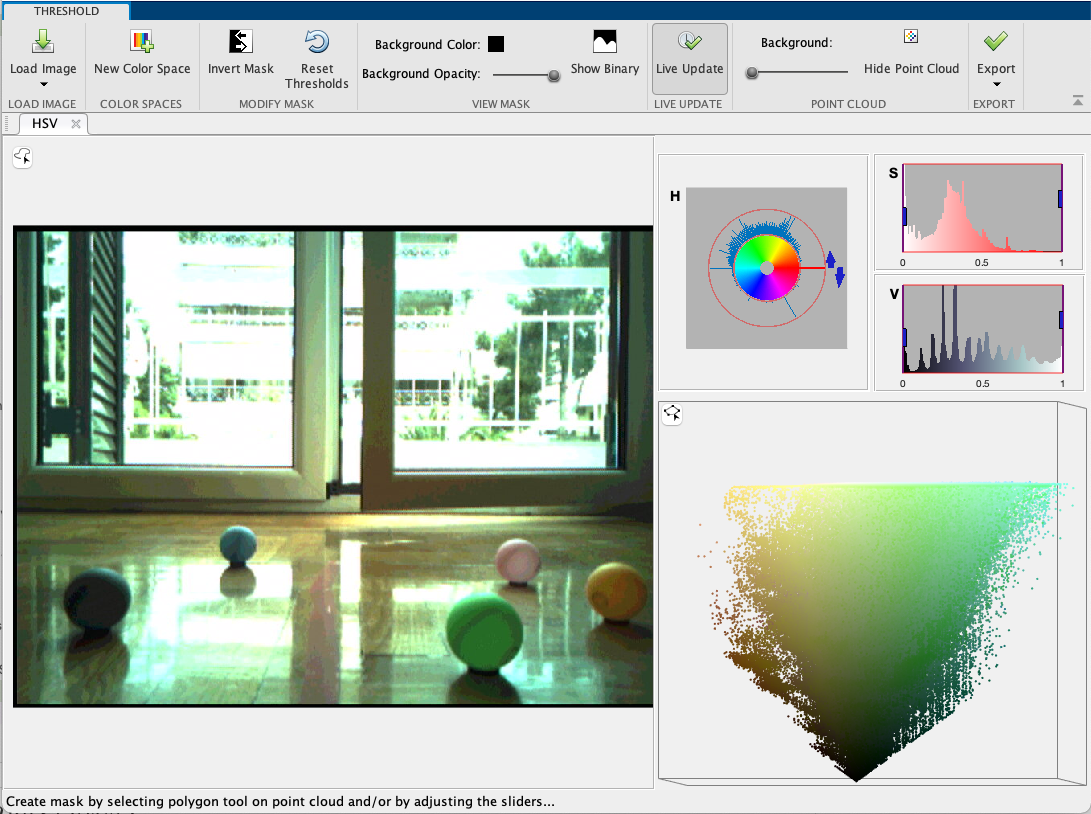
\includegraphics[scale=0.17]{./images/MatlabColourThresholder}
        \caption{MATLAB Colour Thresholder Tool}
        \label{image:MatlabColourThresholder}
    \end{minipage}\hfill
    \begin{minipage}{.5\linewidth}
        \centering
        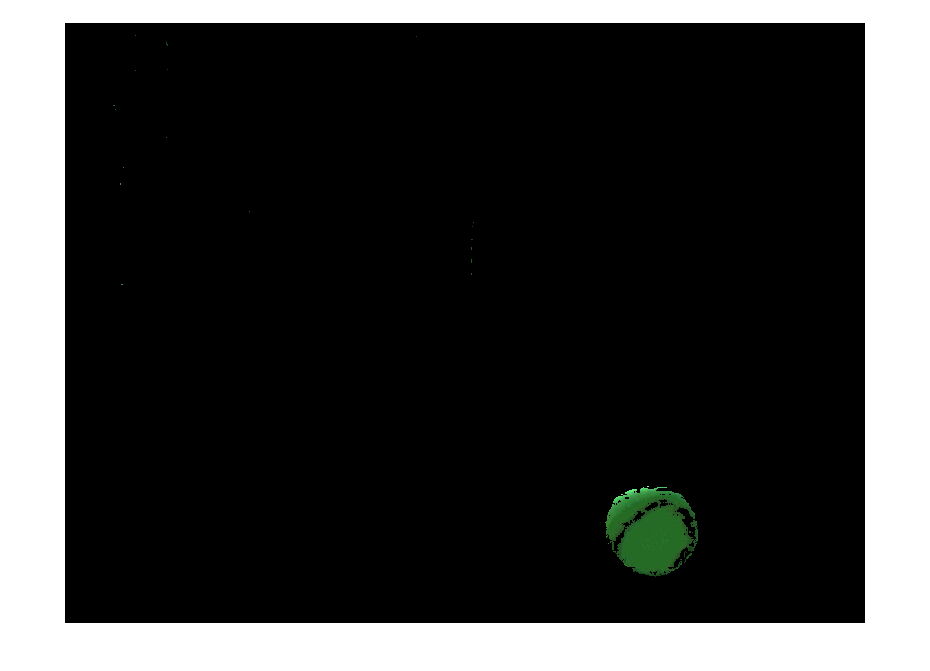
\includegraphics[scale=0.18]{./images/GreenThreshold.png}
        \caption{Tool Produced Composite for Green Ball}
        \label{image:GreenThreshold}
    \end{minipage}
\end{figure}

As can be seen in Figure \ref{image:GreenThreshold}, the tool provides an accurate way to select the values 
for each of the HSV channels, as the binary mode can be used to ensure that the regions
of interest are maximised and the other regions are ignored. 

However, the accuracy of the colour threshold is not perfect for several reasons.
Firstly, even though the HSV colour scheme is used to reduce the effect of illumination, 
the differences in light as the rover approaches the table-tennis balls from different angles
can vary by a large amount, causing differences in the H and S channels, 
hence multiple pictures have to be used for this calibration step. This is also
because the materials used for the construction of the ping pong balls have a specular 
reflectance that causes non-uniform colour dependent on the angle of the light. 
Secondly, as the pictures being used for calibration are from the 4-bit VGA output, 
the output image's colour spectrum is reduced compared to the colour that can be
 ``seen'' by the camera is the full 24-bit colour, that has much more depth and 
a wider range of colours than what is perceived in the output image. Additionally, 
as the data is obtained from the VGA output and captured using an application on 
a computer, there may be some processing that is carried out on the image, meaning 
that the image's data may be different in terms of RGB values from the raw RGB values
that the camera is capturing.

\paragraph*{Use of Pixel Location for Filtering}

A purely colour based pixel approach to object detection has significant flaws unless
the difference between the environment's colours and the object of interest's colours 
are significantly different from each other and the background's colour is plain and
singular. As the testing environment was not ideal, there would be other colours
in the scene that would conflict with the objects causing inaccurate bounding boxes that
were usually too large. In order to filter out these errors and glitches, the 
location of the pixel was taken into account.

Firstly, it was observed that as the testing environment was a flat surface, the 
location of the balls and hence the individual pixels would never be smaller than 
a certain value (since y values are counted from the top down with the top of 
the frame being the 0 value), so this was taken into account and bounding boxes
were only updated on the following conditions: when a colour was detected AND the
video packet was valid AND the pixel y-coordinate \(> 280\). The value of 280 was 
chosen as objects near the horizon level at around 240 pixels would be very far 
away and could be easily mistaken.

This simple adjustment and addition to the object detection algorithm reduced false 
positives by a significant amount. However, it would not be useful if the testing
environment included changes in gradient or if objects of interest were located 
on top of other objects. 

Secondly, as there were still occasional inaccurate bounding boxes, conditions 
were implemented on the software running on the Nios\textsuperscript{\textregistered} II processor to filter out 
boxes larger or smaller than certain values, and boxes that had a ratio that did 
not resemble a square. 



\subsubsection{Object Location Calculations}

With the bounding boxes obtained from the Verilog module, the coordinates of the
bounding box for each colour is sent to the Nios\textsuperscript{\textregistered} II processor using a FIFO buffer.
The calculations for how far away the object is and it's relative position in 
comparison to the camera module was are done on the Nios\textsuperscript{\textregistered} II processor. 

There are multiple ways to calculate the location of a 3D object in space on a plane
with some ways being more precise than others. Some methods rely on using the 
size of a known object and comparing it's relative size in the camera, but the 
decision was made not to use this type of measurement as it was not possible to 
always guarantee that the size of the bounding box would enclose the entire ball, 
making the location calculation inaccurate. 
As the testing environment for the rover was ideal with the camera in a fixed 
position and the testing surface being completely level, the algorithm 
for the mapping between pixel coordinates and real world x-y coordinates relative
to the camera was based on the following form: \begin{align*}
    x & = A_x m^2 + B_x n^2 + C_x mn + D_x m + E_x n + F_x \\
    y & = A_y m^2 + B_y n^2 + C_y mn + D_y m + E_y n + F_y  
\end{align*} This is a relatively simple quadratic mapping between the pixel coordinates 
and the real world coordinate system which is a good choice for this system as the 
Nios\textsuperscript{\textregistered} II is limited in both processing power and available memory. 
By taking a picture of multiple balls in different locations and 
measuring the actual corresponding mapping distance and the pixel locations with
a set of at least 6 measurements, 
the coefficients can be found by solving the matrix equation: $$
    \begin{bmatrix}
        m^2_1 & n^2_1 & m_1n_1 & m_1 & n_1 & 1 \\
        m^2_2 & n^2_2 & m_2n_2 & m_2 & n_2 & 1 \\
        .     & .     &    .   &  .  & .   & . \\
        m^2_i & n^2_i & m_in_i & m_i & n_i & 1 \\  
        .     & .     &    .   &  .  & .   & . \\
        m^2_N & n^2_N & m_Nn_N & m_N & n_N & 1  
    \end{bmatrix}
    \cdot
    \begin{bmatrix}
        A_x & A_y \\
        B_x & B_y \\
        C_x & C_y \\
        D_x & D_y \\
        E_x & E_y \\
        F_x & F_y
    \end{bmatrix}
    =
    \begin{bmatrix}
        x_1 & y_1 \\
        x_2 & x_2 \\
        . & . \\
        x_i & y_i \\
        . & . \\
        x_N & y_N
    \end{bmatrix}
$$ where the pixel locations are represented by \((m,n)\) and the physical locations on
the plane are represented by \((x,y)\). Initially 6 samples were taken to calculate 
the coefficients, but as more measurements were taken to verify the method, they
were also added to the list of samples to improve the accuracy of the algorithm.
It was noted during initial testing that balls at a further distance were located
more accurately than balls closer together, the cause of this problem was because
the calibration data had more data points at a further away distance, causing the mapping
to prioritise accuracy there, this was then fixed by adding more data points for 
balls that were closer to the camera. 
These calculations for the coefficients were carried out in MATLAB, and then 
implemented in C to be run on the Nios\textsuperscript{\textregistered} II processor. 

The Nios\textsuperscript{\textregistered} II processor does not include floating point hardware by default, but as 
this algorithm requires floating point calculations as some of the coefficients 
tend to be very small, and this algorithm is run for each set of colours, it was
prudent to include hardware support for single precision floating point adds 
and multiplications. This was done by adding the Nios\textsuperscript{\textregistered} II Custom Floating Point Instruction module from Intel's IP catalogue 
for custom floating point instructions, which reduces the amount of cycles 
necessary to carry out a floating point multiplication to 4 cycles using a single
instruction and a floating point add to 5 cycles\cite{NiosIICustomInstruction}.
If this hardware was not used, it would be implemented using software, and hence
would take multiple instructions and more hence more cycles. 

This method is satisfactory in its performance, with a worst case error of \(\pm5\unit{cm}\)
in difference between calculated position and actual position when the bounding box is accurately detected. 
For the rover's path finding algorithm, this is a value that is easily taken into account and as
multiple measurements of the ball are taken, the actual position can be refined 
and more accurately determined by taking the average of multiple readings in the 
Command module in the server. This also solves the problem of when a ball is not 
fully in the frame of the camera or not fully detected by the object detector,
as the rover is moving, all objects should eventually come into frame fully and 
not be cut off by the sides of the view or receive a better view of the object 
leading to a better bounding box and hence distance calculation. 
Additionally, this algorithm's performance is ideal in the current testing environment, 
but if tested on a surface with changing gradients or elevated objects, this algorithm
would be inaccurate due to it's inability to take into account objects on the real
world z-axis (i.e. the height of an object relative to the plane).





\subsubsection{Image Transfer over SPI}

To be able to send an image to the Command view for the user to view is an essential
part of a Mars Rover's mission, thus it was one of our goals to do this as well. However,
due to time limitations and other operations that took priority, there was not enough time
 to and memory available on the FPGA to implement it fully. 

In order to facilitate this function, a custom SystemVerilog module was designed specifically 
for sending an image via SPI. The image parameters as aforementioned are \(640 *480\) at 60fps 
with 8 bits of colour for each channel. This requires 921,600 bytes per frame which is just 
under a 1kb per frame. Usually, for sending image data, before the data transfer happens, 
compression is applied on the sender's side before compression, but as memory and processing
power is limited, it is not possible to implement any sort of encoding onboard the FPGA and the
only option is to offload it to either the ESP32 or the webserver for encoding and display. 

The module's structure is shown in Figure ... It acts as an SPI peripheral that provides 
data whenever it is read from by an SPI controller, with pixel values being stored in a FIFO 
buffer that is written into by the image processing module. 26 bits are stored within the FIFO
with the first two bytes used to indicate a start of frame or an empty FIFO, this indicates to the 
SPI controller the position of the image and also when to stop asserting the sck to indicate that 
transmission should stop. The FIFO used is a dual-clock FIFO that uses the main clock as the input
clock and the sck provided by the SPI controller is used as the clock for the read.  


\subsection{Integration}
The purpose of Integration is to ensure and test the work of all the subsystems together. The following section is organised in a 
way that shows the progress of the system and all the testings and measurements done to allow the delivery of this working system. 
The good communication and will to work hard that was shared by all the team members was a crucial factor that led to the completion of the tasks.

\subsubsection{Drive}
Having an accurate and reliable driving system was the first important milestone for this project as it is the means of the Rover to navigate its environment.
The first test done to ensure that was measuring fixed distances traversed by the Rover and callibrating the optical flow sensor using the sample code. The testing procedure was fairly simple but produces consistent results.
By using some fixed tiles on the floor that have a dimension of \(25cm\times 25cm\). By using these I could measure how accurate the Rover moves and rotates and also minimizing human errors that would arise if the reference distance and angle was not in place. 
The first problem that arised was an error in distances greater than \(20cm\) where there was a sudden sign change  in the measured distance of the sensor.
\begin{figure}[H]
    \centering
    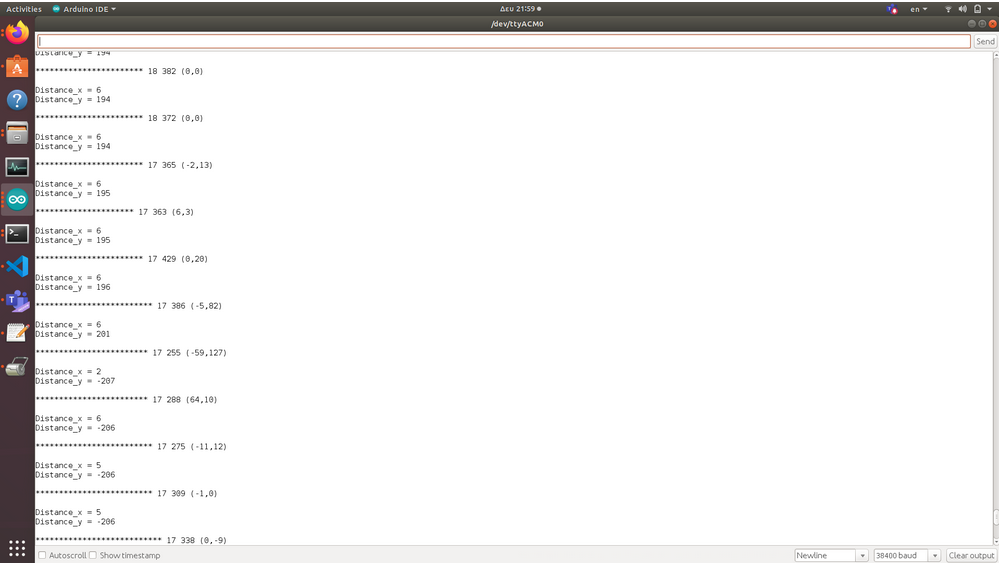
\includegraphics[scale=0.3]{./images/overflow_example.png}
    \caption{Serial Monitor output showing the overflow of distance.}
    \label{image:Overflow of Distance}
 \end{figure}
As it can be seen in Figure ... the distance measured went from \(201mm\) to \(-207mm\) which indicated a bug. I communicated my foundings with the member that 
was in charge of Driving and we concluded that it is an overflow caused by the multiplication operations of the code which can be easily fixed by prioritising divisions.

After having received the fixed code and continuing testing it was concluded that the floor material affects the optical flow sensor's accuracy greatly. Trial and Error showed that the best floor material in the area of testing operations was wood which gave the most reliable readings.
Having a proof of concept is crucial when deciding to move to more complex operations for the system and during the initial testing of the Drive module, it was concluded that it had a good accuracy that would be essential for the later stage of mapping the balls.

When trying to measure considerably bigger distances with the Rover, it was identified that the strain from the cables connected could impose some considerable torques on the system which could result in innacuracies.
This could possibly be solved by implementing a PID that ensures no rotation while moving forward and backward, but after consultation with the appropriate team member it was decided that because the purpose of the cables is for debugging, capturing of data and supplying power, in a real-life scenario it would not affect the rover.
For the demonstration and all the testing it was also decided that the cables should be placed in positions that would cause minimal strain in the system. 

After ensuring that the navigation of the Rover is accurate enough, the next logical step is to test and implement the communication procedure with the control module.
\subsubsection{Communications between Drive and Control}
Knowing that the team member in charge of Control only has the ESP32 board, it was crucial to establish a close contact so that the feedback from the Integration testing is relayed back and used to improve the Control code.
Having a Rover that can navigate is important, but there needs to be a communications framework that will allow it to receive and execute commands. When researching the different communication protocols, it was concluded that UART is a reliable and good hardware device that allows the transmission and reception of data. After consulting with the team member of Control and receiving the available UART pins of the ESP32, the cable connections were made. 
\begin{figure}[H]
    \centering
    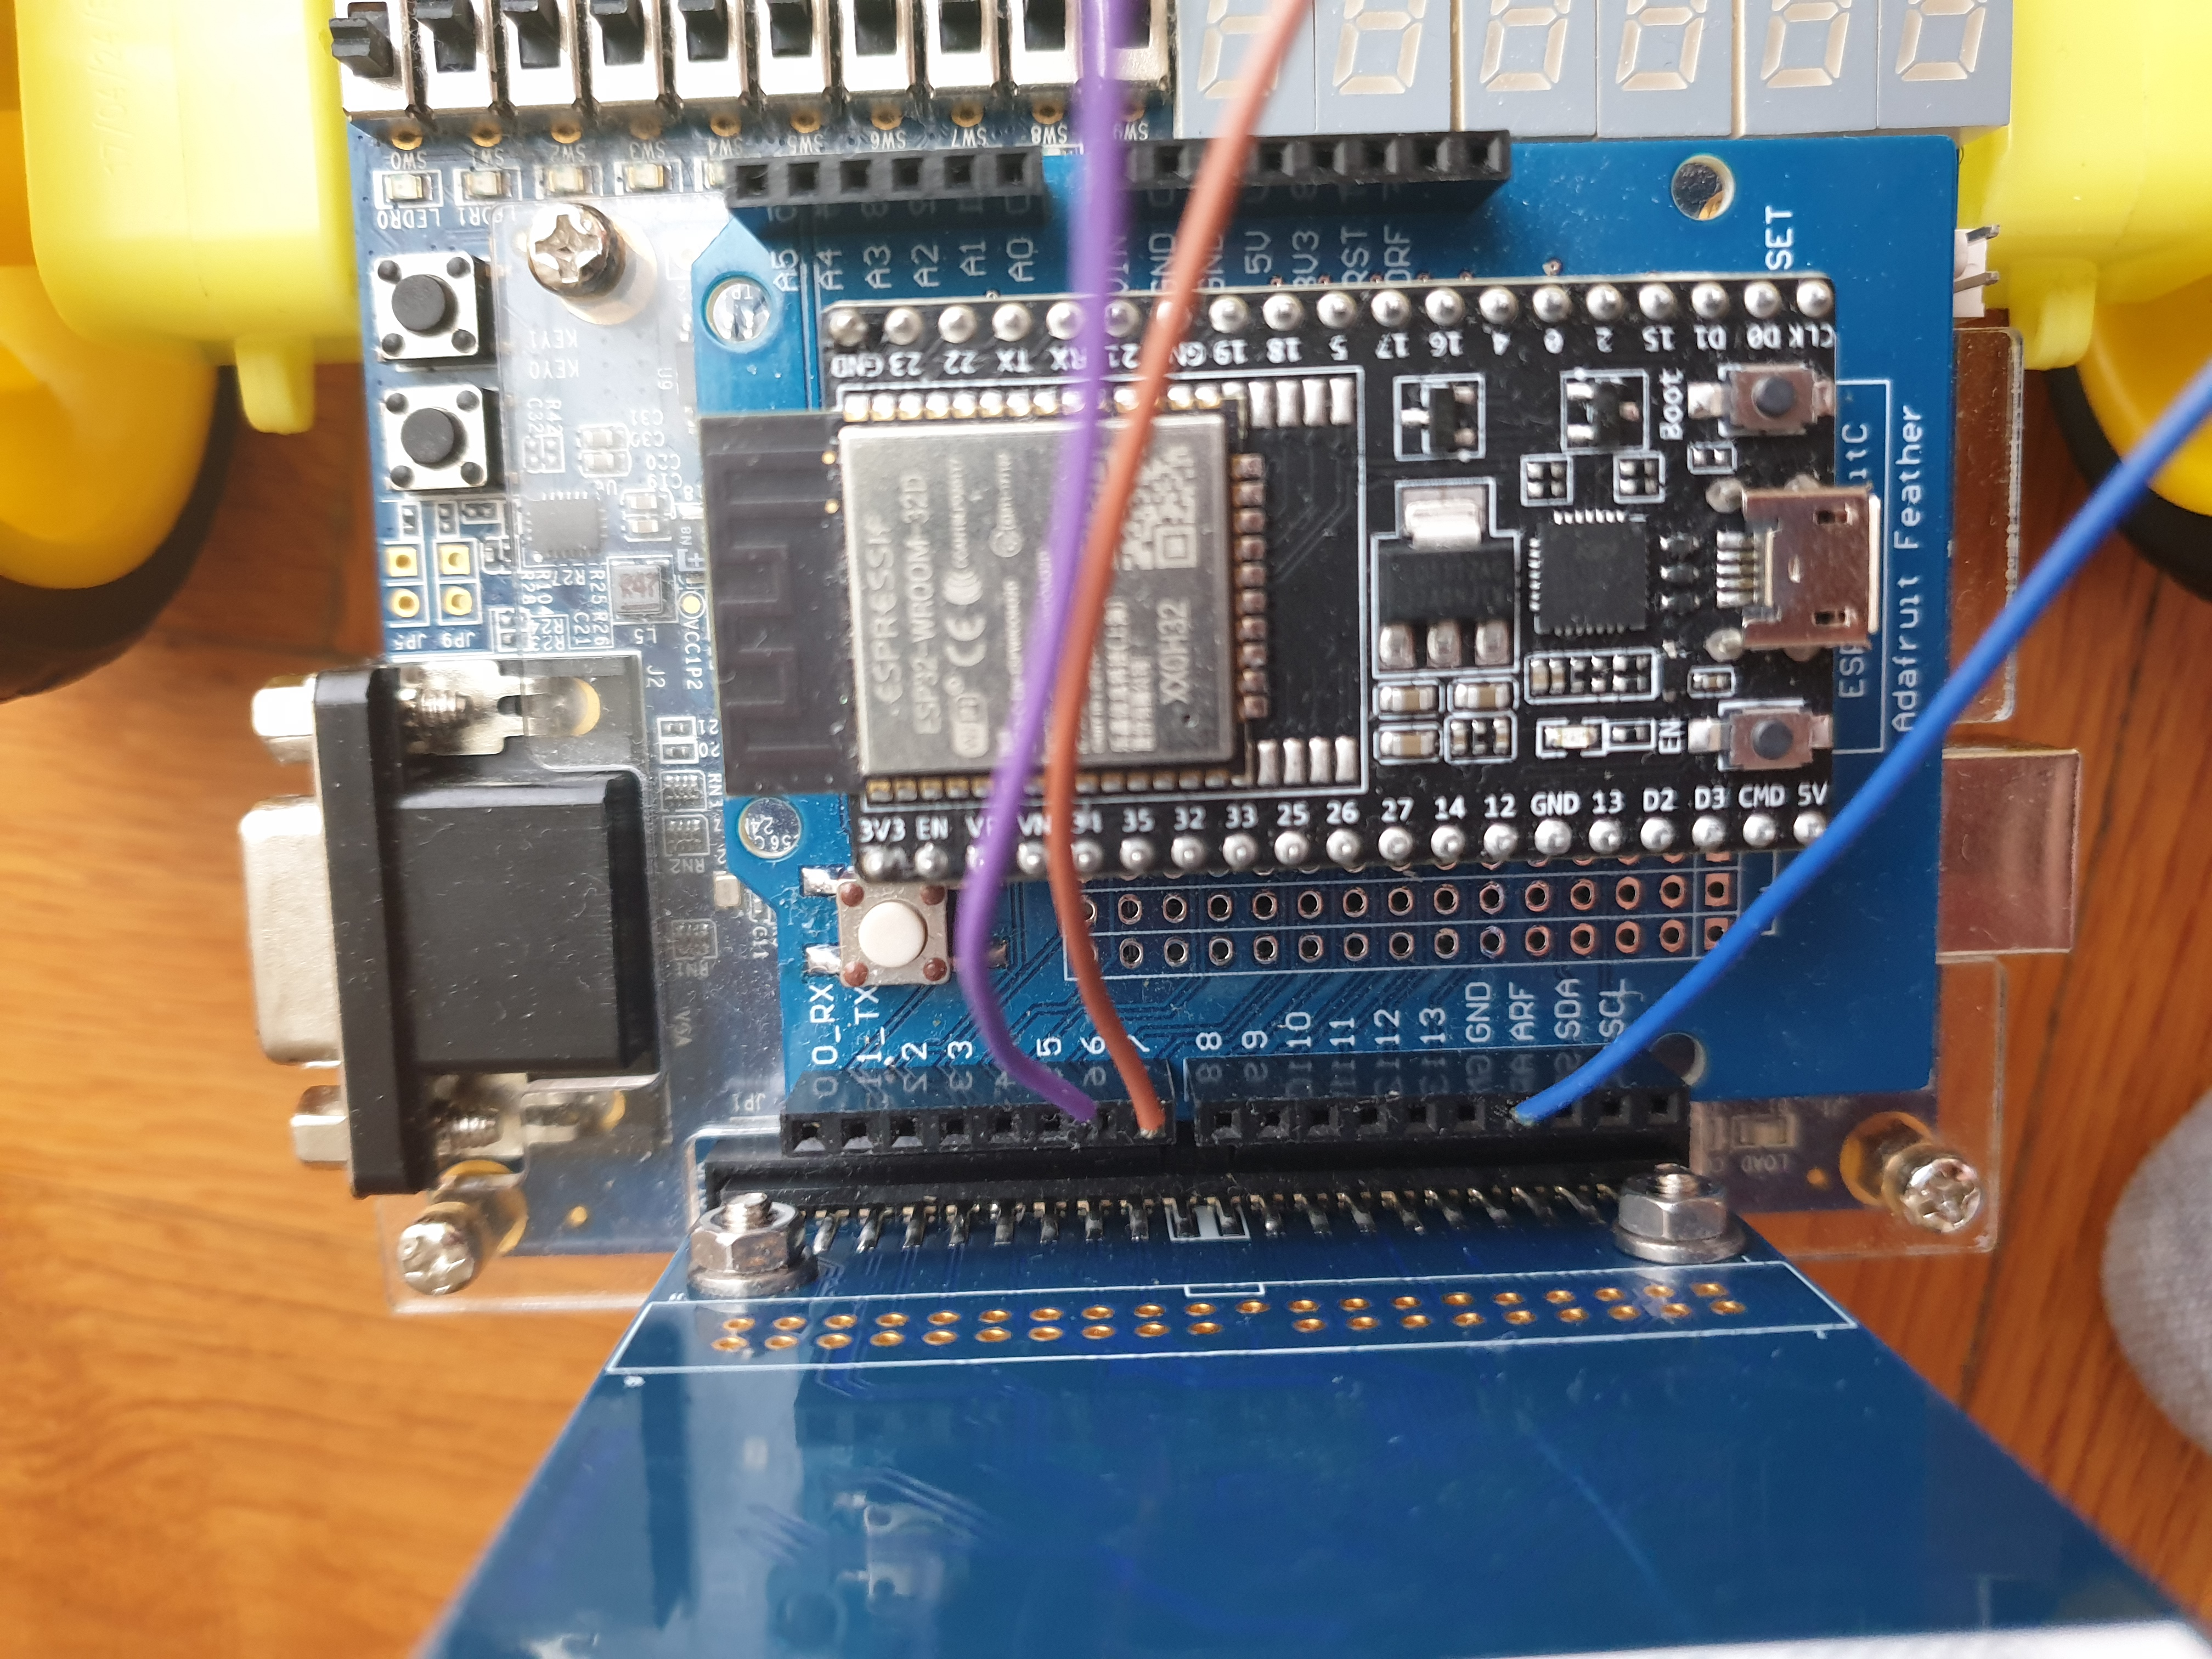
\includegraphics[scale=0.05, angle = 180]{./images/ESP32_UART.jpg}
    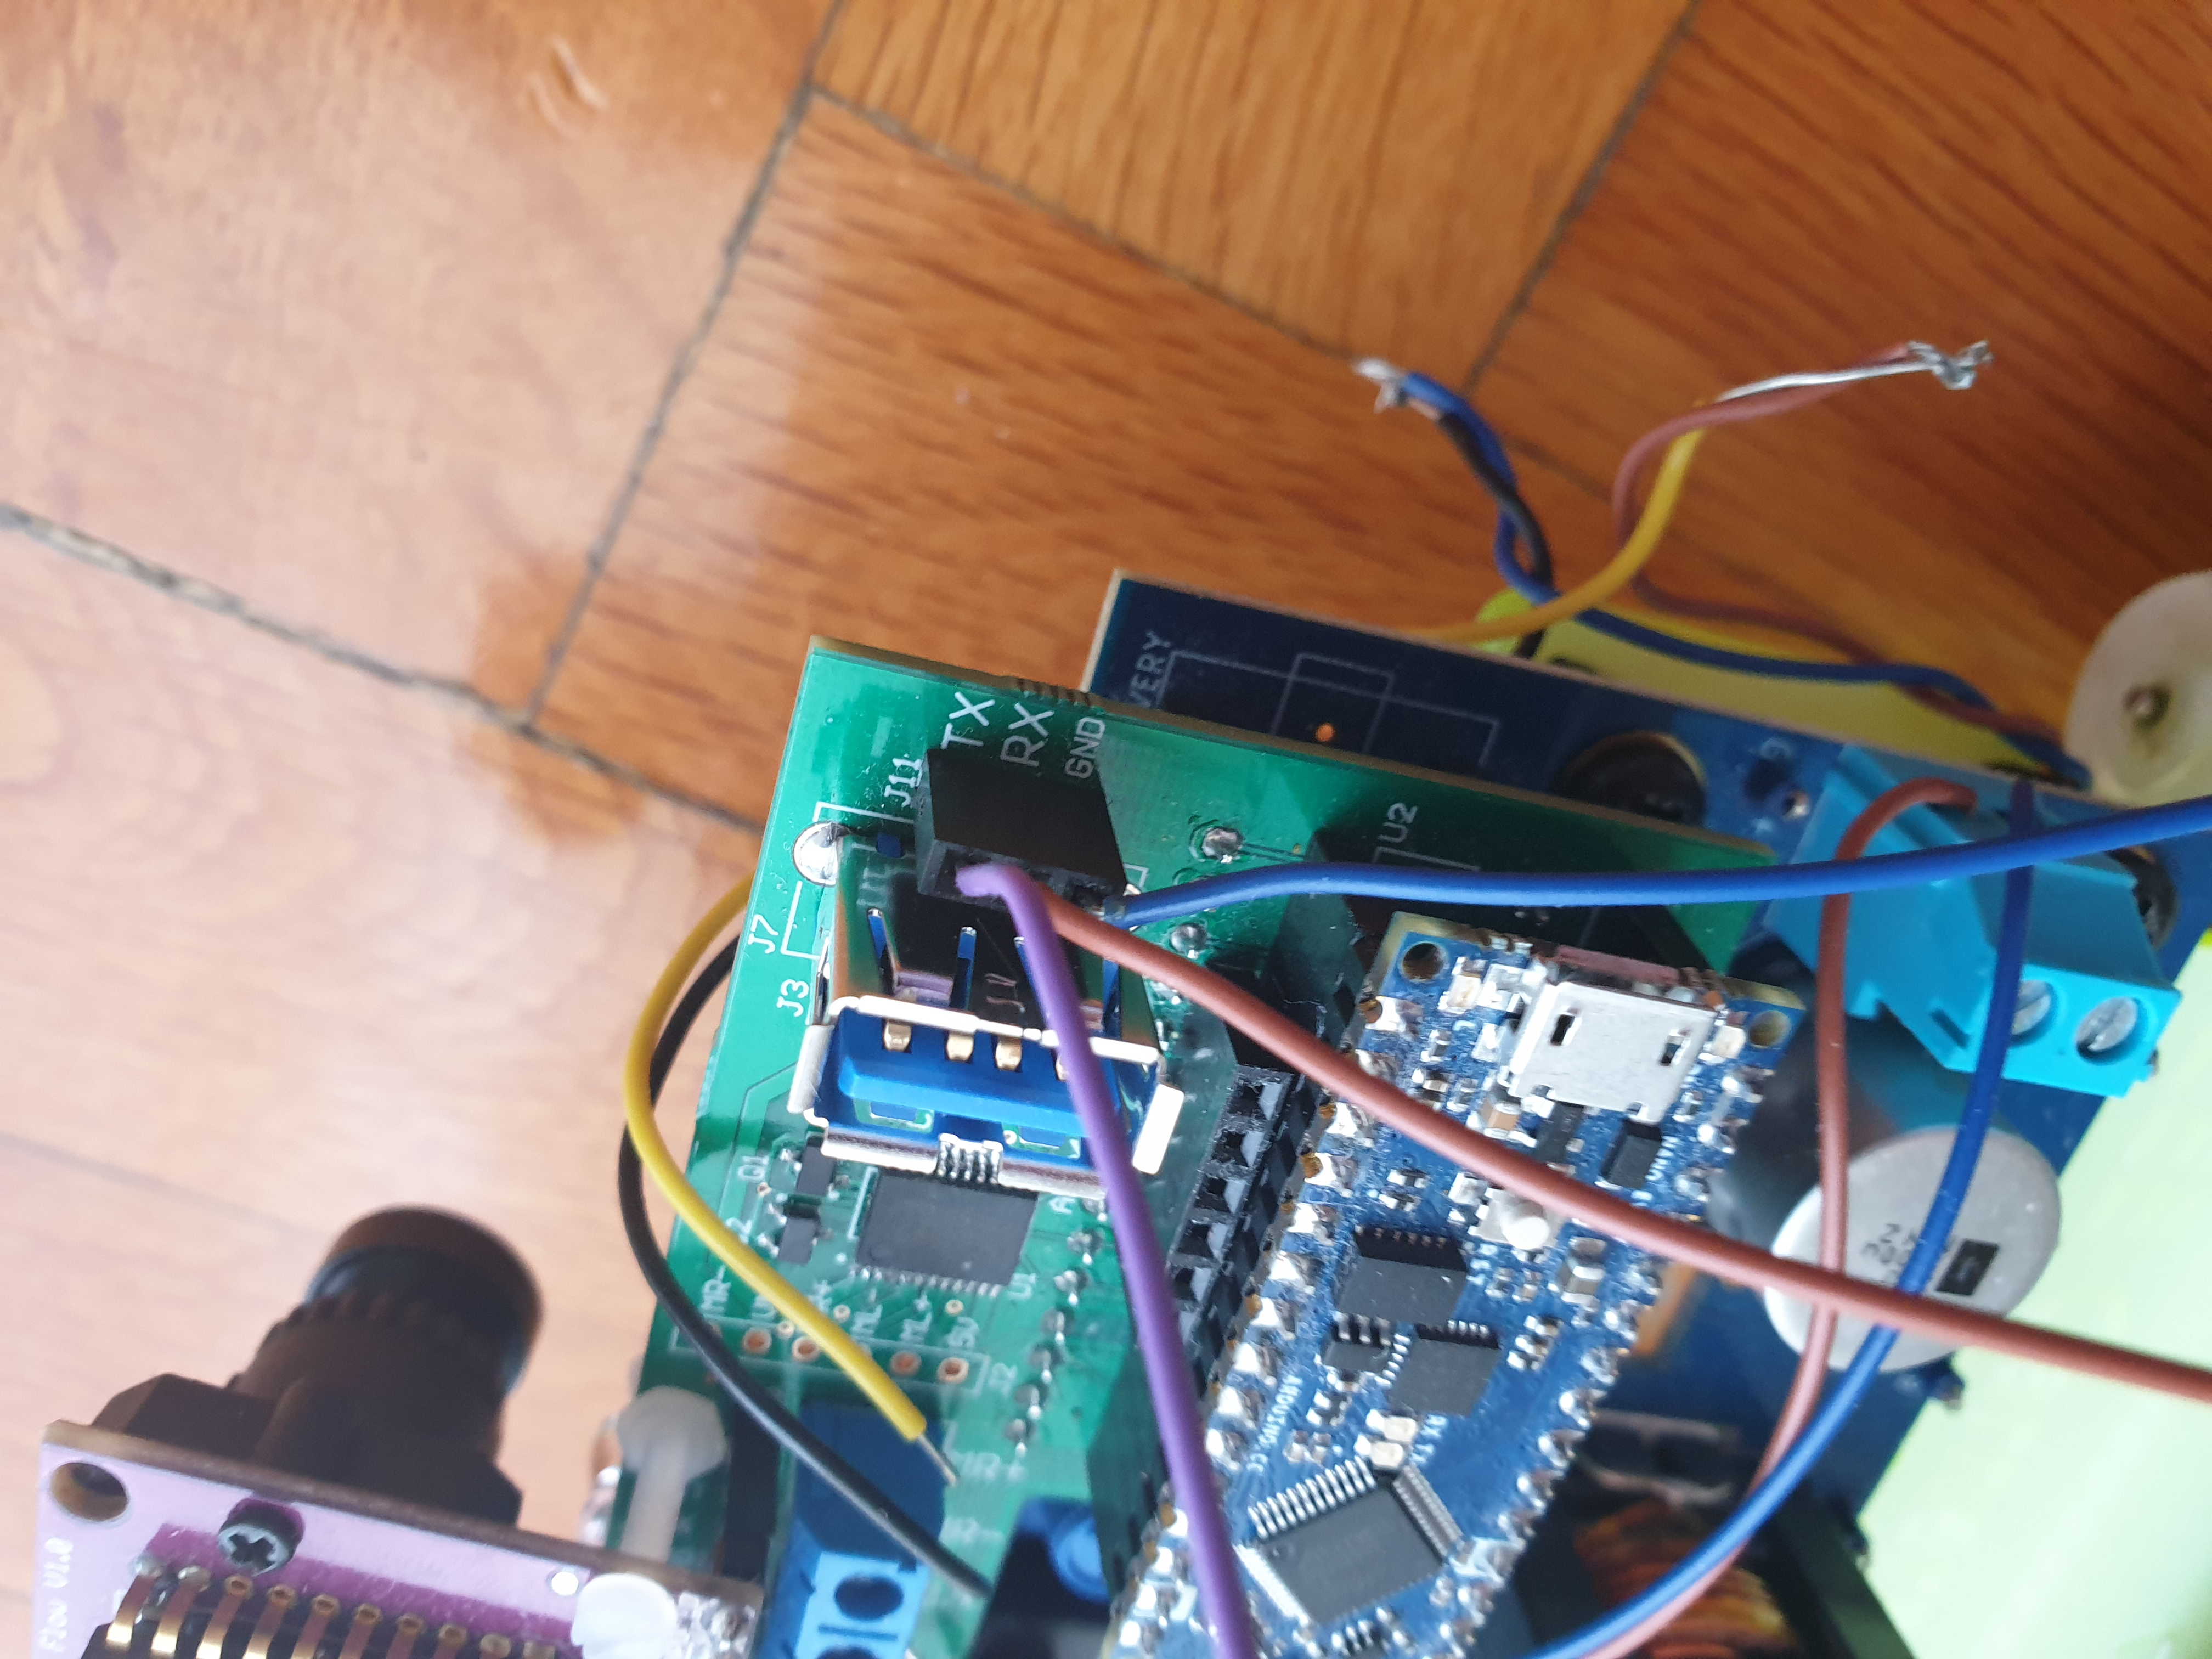
\includegraphics[scale=0.05, angle =  180]{./images/Arduino_UART.jpg}
    \vspace{-10pt}
    \caption{From left to right: ESP32 cable connection to UART pins,Arduino Nano Every cable connection to UART pins.}
    \vspace{-10pt}
    \label{image:UART}
\end{figure}
\begin{figure}[H]
    \centering
    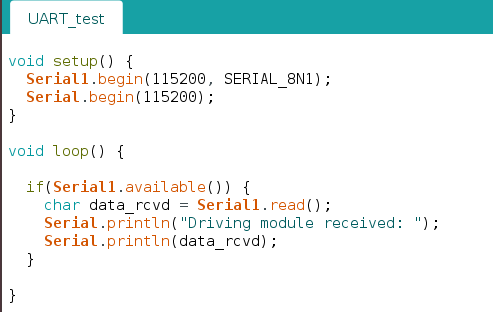
\includegraphics[scale=0.5]{./images/UART_test.png}
    \caption{Test code to ensure UART functionality}
    \label{image:Simple UART test}
 \end{figure}
To test the connection, a fairly simple program was made that reads the Serial buffer when it is available. To achieve reliable Integration of the systems, a modular approach is chosen where the testing of even the simplest components is of great importance.
This is to confirm funcionality and detect faulty hardware without having to debug complex programs that may or may not contain bugs.
After ensuring UART functionality, a more complex program was implemented to allow driving to receive commands from Control. 
\begin{figure}[H]
    \centering
    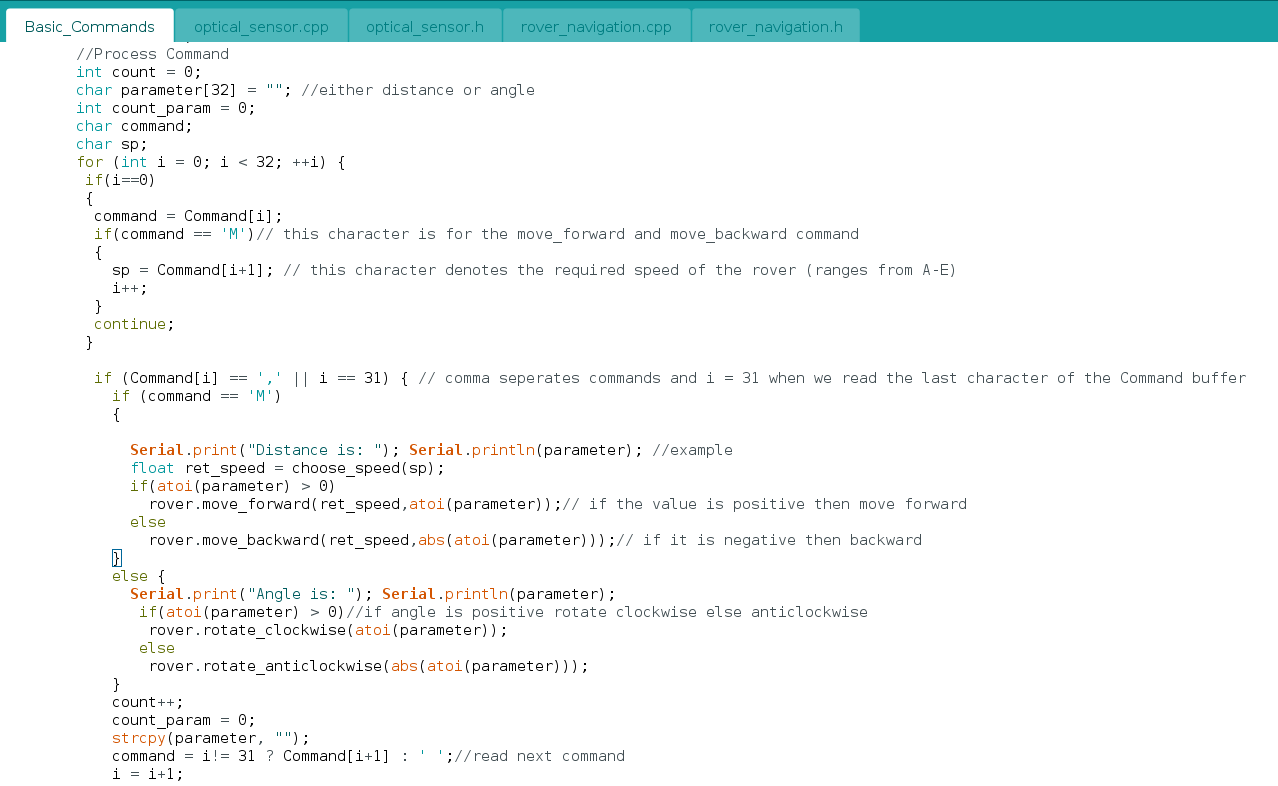
\includegraphics[scale=0.3]{./images/Command_decoder.png}
    \caption{Command decoder}
    \label{image:Code flashed on Arduino}
 \end{figure}
 The command structure was fairly simple and not resource heavy. The Rover does a series of rotations and movements. The starting character of a command is \("["\) which allows the system to identify the start of a command being transmitted by Control. To move the Rover a transmitted character should be \(M\) and after that the speed should be identified using a character between \("A-E"\) with \("A"\) being the fastest available option and \("E"\) the slowest.
Because rotations are the only other option, an arbitrary character can be used acompanied with the angle of rotation. The code also handles signs denoting direction of rotation and movement.
For example, \("[MA300,R-90]"\) is a command that when executed by the Rover will result in a forward movement of \(300mm\) and an anticlockwise rotation of \(90\) degrees.
Lastly, to allow for flexibility of commands, a stop functionality was added when Control sent the character \("S"\) while executing a movement command which stops the motors and transmitts the distance covered back to Control.
\begin{figure}[H]
    \centering
    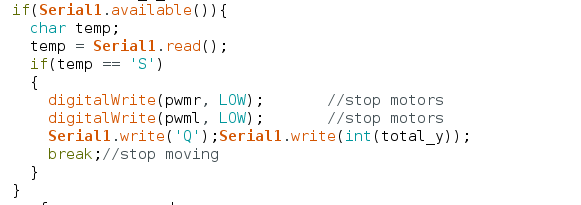
\includegraphics[scale=0.5]{./images/Stop_functionality.png}
    \caption{Command decoder}
    \label{image:Code flashed on Arduino}
 \end{figure}
%Start of energy implementation
\subsection{Energy}
\vspace{-10pt}
\begin{figure}[H]
    \centering
    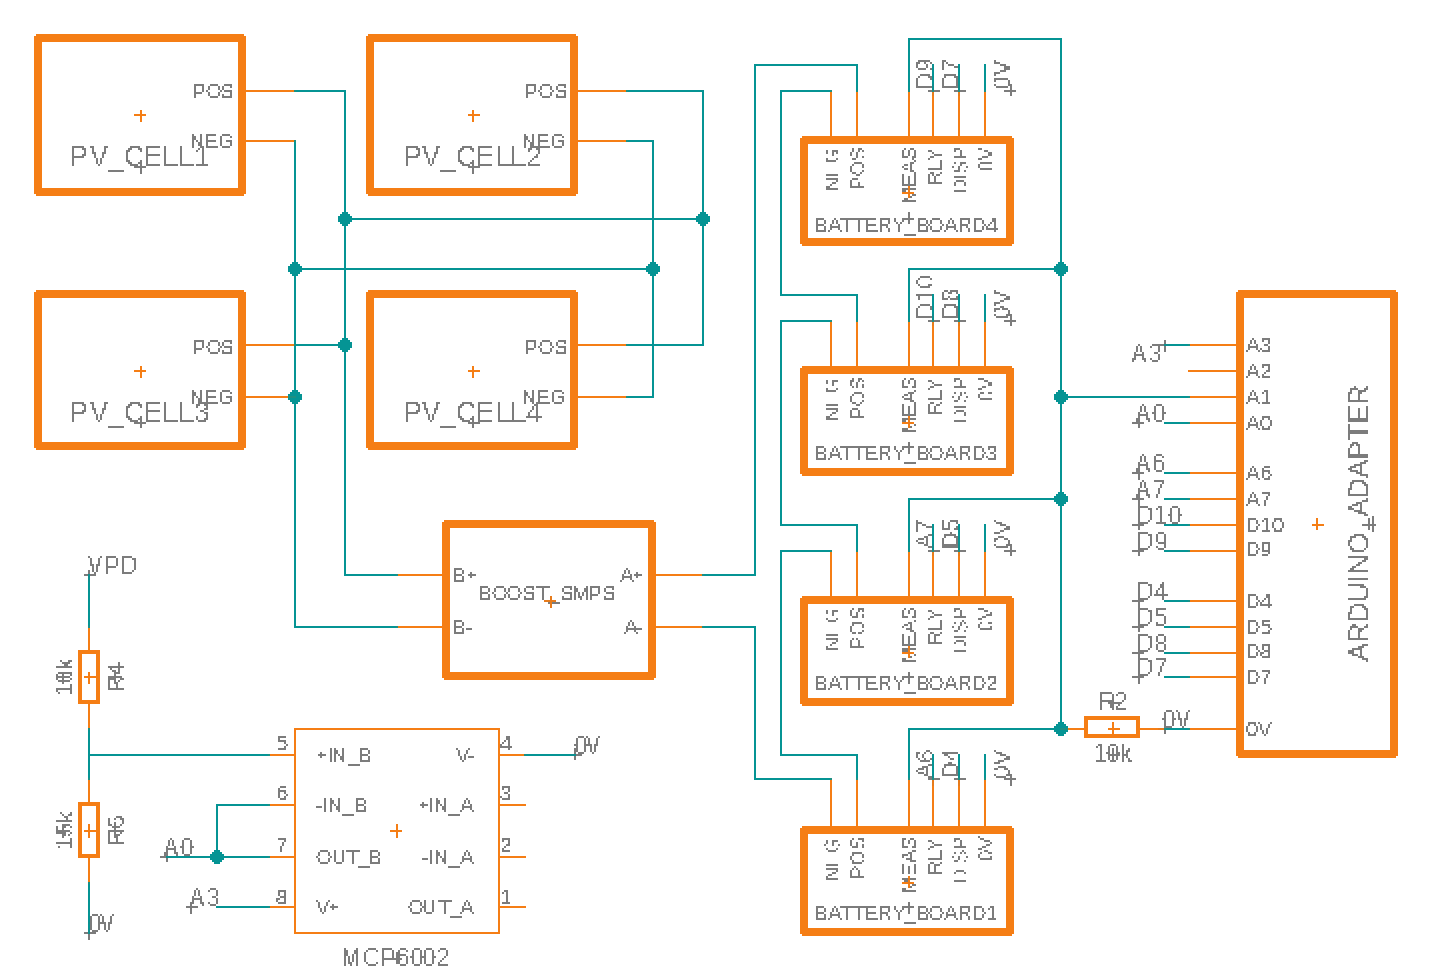
\includegraphics[width=0.8\textwidth]{Circuit_Diagram.png}
    \caption{Circuit diagram of the finished energy system.}
    \label{fig:circuitDiagram}
\end{figure}

\paragraph*{SMPS Configuration}
The voltage of the series battery pack is higher than the voltage of 
the parallel connected PV panels. The voltage of the PV array must 
therefore be stepped up before it can be used for charging. The SMPS 
is therefore operated in boost mode with the PV panels connected on 
port B and the battery on port A. Moreover, as the SMPS has a max 
output voltage of 7 V in synchronous boost mode\cite{powerLogbook}, 
non-synchronous mode was used. Finally, the on/off switch was set 
to emph{off} such that all power comes from the PV array and not 
from the USB connection powering the Arduino.

\paragraph*{Measurements}
Measurements of the circuit currents and voltages are used to track the 
operation of the subsystem. During charging, the most important measurements 
are the output voltage, the cell voltages, and the battery current.

The battery voltage is usually in the range 10.0 to 14.4 V. However, 
the Arduino can only measure voltages up to 4 V. To solve this issue 
the output voltage was passed through a voltage divider. The voltage 
divider consist of two parts. Firstly, a 560 $\Omega$ and a 330 $\Omega$ 
resistor create $V_{pd} \approx 0.37 * V_{out}$. $V_{pd}$ is then reduced 
even further using a 15 $k\Omega$ resistor and a 10 $k\Omega$ resistor 
to $\sim 0.22 *V_{out}$, which is then passed to the Arduino. With this 
voltage divider it should be possible to measure output voltages up to 
18 V. The second stage uses far large resistors than the first so that 
the two do not impact one another. However, due to the large resistance 
values, the current drawn by the Arduino during sampling would cause a 
significant voltage drop. To prevent this an op-amp from the Circuits lab 
was used to buffer the voltage before it was connected to the Arduino.

The measurement port on the battery boards is used to measure cell voltages. 
To use this port the battery board relay is be switched by setting 
the \emph{RLY} input \emph{HIGH}. While the relay is switched the battery 
cell will be disconnected from its power terminal. For a series battery 
pack this means that the cells can only ever be measured or 
charged/discharged at a given time. To have the smallest impact on 
operation the measurements are therefore completed as quickly as possible 
and taken at a low frequency. To measure the voltage of a cell the first 
step is to set the output current to 0 mA to prevent voltage spikes 
while the battery is disconnected. The relay is then switched, the 
voltage is sampled and the relay is switched back. When abiding by the 
switching times of the relay and giving time for the current/voltage to 
stabilise this process takes about 40 ms. To minimise the number of 
Arduino ports needed for measurements, the cell voltages are not measured 
at the same time. Instead, one cell is measured every second. As there 
are 4 battery cells this means that each cell is measured with 4 second 
intervals. Due to the cell voltages changing very slowly the long update 
time was not found to be a problem.


The current in and out of the battery needs to be tracked to determine 
the SOC. However, the current sensor is on the wrong side of the SMPS 
to measure the current flowing into the batteries. Initially this 
problem was solved by connecting a 0.5 $\Omega$ resistor between the 
SMPS output and the battery. By measuring the voltage across this 
resistor the current into the battery could be determined. Initial 
tests of this solutions gave promising results. However, an excessively 
complex circuit was needed to ensure the sensor worked for both positive 
and negative currents. It was determined that a better solution was to 
simply calculate the output current from the input current using the 
formula \( I_{out} = (1 - \delta)*I_{in} \). A problem with this solution 
is that it assumes CCM. At the standard charging current of 250 mA this 
assumption holds, but for smaller current, below about 150 mA, the SMPS 
might enter DCM. In this case the calculated current will be somewhat 
higher than its true value, which might impact SOC tracking. However, 
as will be discussed, the SOC algorithm has methods for correcting 
itself and this will hopefully mean that the error does not get too 
big. Unfortunately, it was not possible to test this due to the ban 
on working with batteries.  

\paragraph*{Controlling the SMPS}
The dual loop controller from the sample charging code\cite{chargeCode} was 
used as the starting point for the controller design. However, some 
changes were necessary to accommodate other design choices. As previously 
discussed, the current needs to be set to 0 for only a couple of 
milliseconds when cell voltages are being measured. This is not 
possible using the 1 Hz Moore machine from the original controller. 
As such the slow loop was changed to a Mealy machine, where the 
outputs could change with the clock speed of the fast loop. This had the 
unfortunate side effect of creating timing issues as the resulting 
code was too complex for the Arduino to successfully run the fast 
loop at 1 kHz. For this reason the clock speed of the fast loop was 
reduced to 500 Hz. It should also be noted that the PI-gains from 
the sample code were changed as they did not work optimally in boost 
mode. The new gains were found through trial and error.

\paragraph*{Charging Algorithm}
\vspace{-20pt} 
\begin{figure}[H]
	\centering
    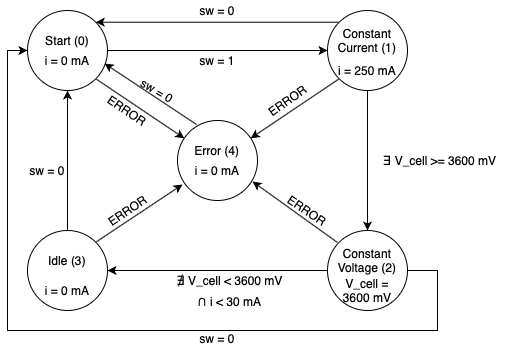
\includegraphics[scale=0.5]{State_diagram.png}
    \caption{State machine of the charging algorithm.}
\end{figure}
\vspace{-20pt}
The battery cells are designed to be charged first with a constant current and then 
with a constant voltage of 3.6 V\cite{batteryDatasheet}. The implemented charging 
algorithm follows this specification as much as possible. The state machine starts 
in state 0 where the output current is set to 0. It waits in this state until the 
OL/CL switch is set to 1, after which it moves to the constant current state. 
In the constant current state the current is nominally 
250 mA. However, as will be discussed later, if the solar panels do not produce enough
power to charge at 250 mA, the MPPT algorithm might impose another lower value for 
the constant current in this state. Moreover, technically the current is not 
constant as 40 ms of each second is used to measure cell voltages, and for a 
short period there will be zero current. These short charge breaks were not found 
to have an impact on the performance of the charging process. In fact, 
charging $LiFePO_{4}$ battery cells with a pulsating current has even been 
found to severely reduce battery degradation\cite{PulseCharging}, which might 
mean better performance than truly constant current in the long term. The 
charging algorithm leaves the constant current state for the constant voltage 
state once any cell reaches a cell voltage of 3600 mV.

Initially the output voltage was kept constant in the constant voltage 
state. However, even if the voltage across the battery pack as a whole is 
constant this does not mean that the voltage across individual cells is constant. 
Testing revealed that with a constant output voltage, weaker cells could sometimes 
reach a cell voltage over 3700 mV as current died down. To prevent this, the 
constant voltage state was redesigned from keeping the voltage across the battery 
pack constant, to trying to keep the voltage of each individual cell constant. 
This was done in two steps. Firstly, the battery input current is regulated so 
as to keep the highest cell voltage in the range 3600 to 3630 mV. Secondly, 
balancing ensured that cells of lower voltage catch up to the highest voltage. 
The code used to control the constant voltage state is shown in 
Figure~\ref{fig:Constant_Voltage}. Initial test of this code gave promising 
results, but it could not fully be tested due to the ban on working with 
batteries. However, Figure~\ref{fig:balancing} shows the ability of the code 
to stabilise all cell voltages around 3600 mV. After all cell voltages have 
reached 3600 mV and the current has died to below 30 mA, the charging algorithm 
is done and the state machine enters an idle state. 

\begin{figure}[H]
    \centering
    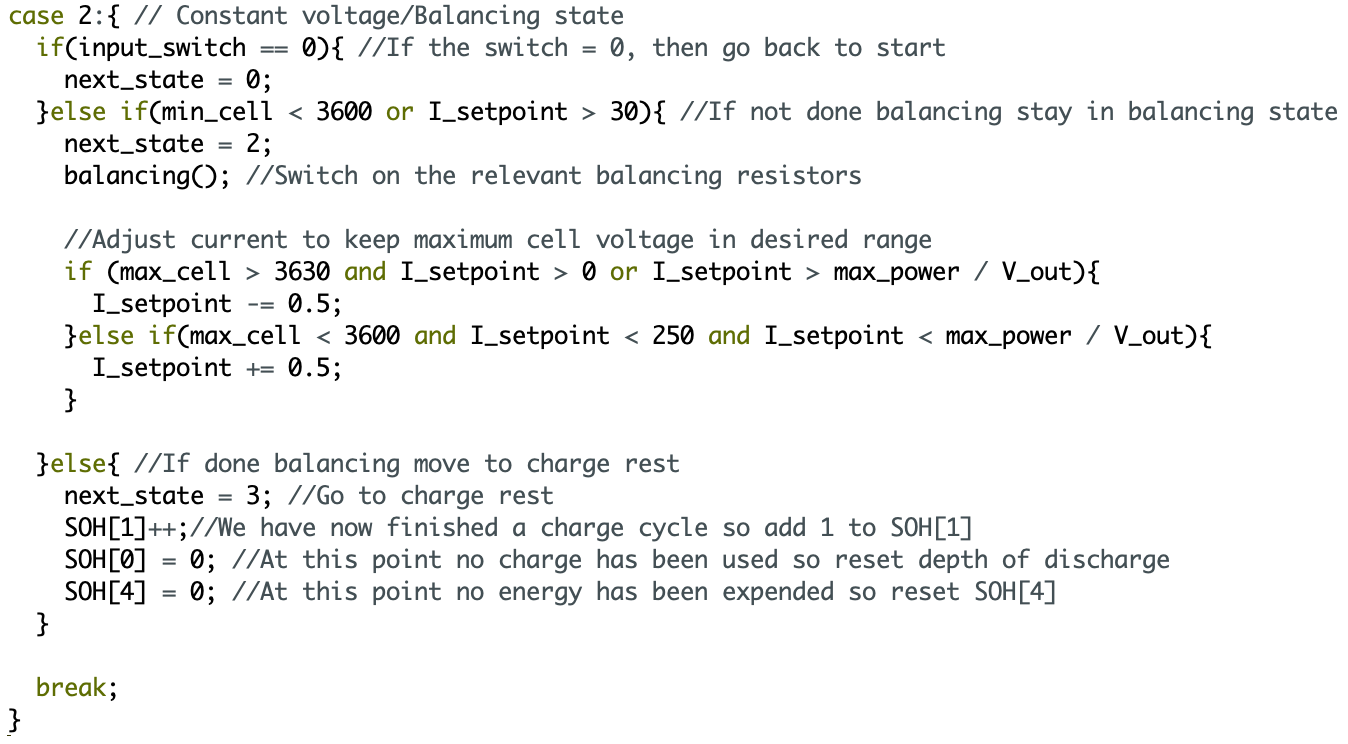
\includegraphics[width = 0.7\textwidth]{Constant_voltage.png}
    \caption{Code used to keep cell voltages constant.}
    \vspace{-10pt}
    \label{fig:Constant_Voltage}
\end{figure}

\paragraph*{SOH and Cell Balancing}
To monitor the battery’s SOH the charge capacity, energy capacity, 
cell voltage balance, and the number of completed charge/discharge 
cycles are all tracked. To retain the data between sessions, it was 
logged in a CSV format to the SD card every 60 seconds. The relevant data 
was then read in from the SD-card on start up.

To maintain SOH the cell voltages were balanced every charge cycle. 
As previously explained balancing should only occur at high SOC, 
which is why balancing is only done in the constant voltage state. 
The code use for balancing is shown in Figure~\ref{fig:balancingCode}. 
During CV charging it is desirable that all cells have a voltage of 
3600 mV. If any cell has a voltage which is higher than 3600 mV, 
its voltage is too high and the dissipative resistors are switched 
on to lower the voltage. When used in conjunction with the constant 
voltage charging algorithm this code was extremely successful at 
balancing the cells. The balancing is shown in action in 
Figure~\ref{fig:balancing}. As can be seen, the cell voltages are 
one by one brought up to and kept at 3600 mV. Even with an initial 
voltage difference of 200 mV, the balancing only takes about 
1000 seconds = 17 minutes. 
 
\begin{figure}[H]
    \centering
    \begin{minipage}[b]{0.49\textwidth}
        \raisebox{30pt}[\dimexpr\height-3\baselineskip\relax]{%
        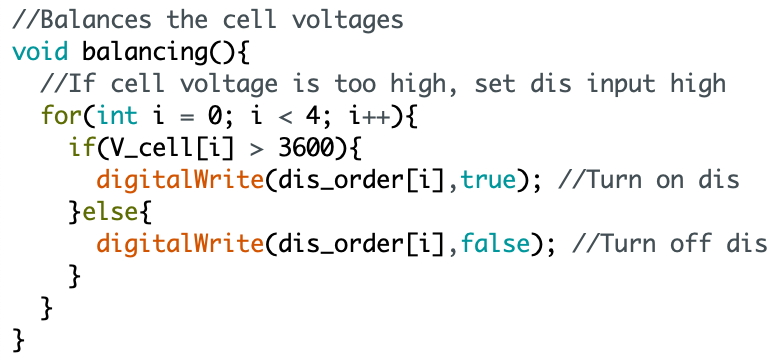
\includegraphics[width=\textwidth]{Balancing_code2.png}
        }%
        \caption{Function called while charging at high SOC to balance out the voltage of the cells.}
        \label{fig:balancingCode}
    \end{minipage}
    \hfill
    \begin{minipage}[b]{0.49\textwidth}
      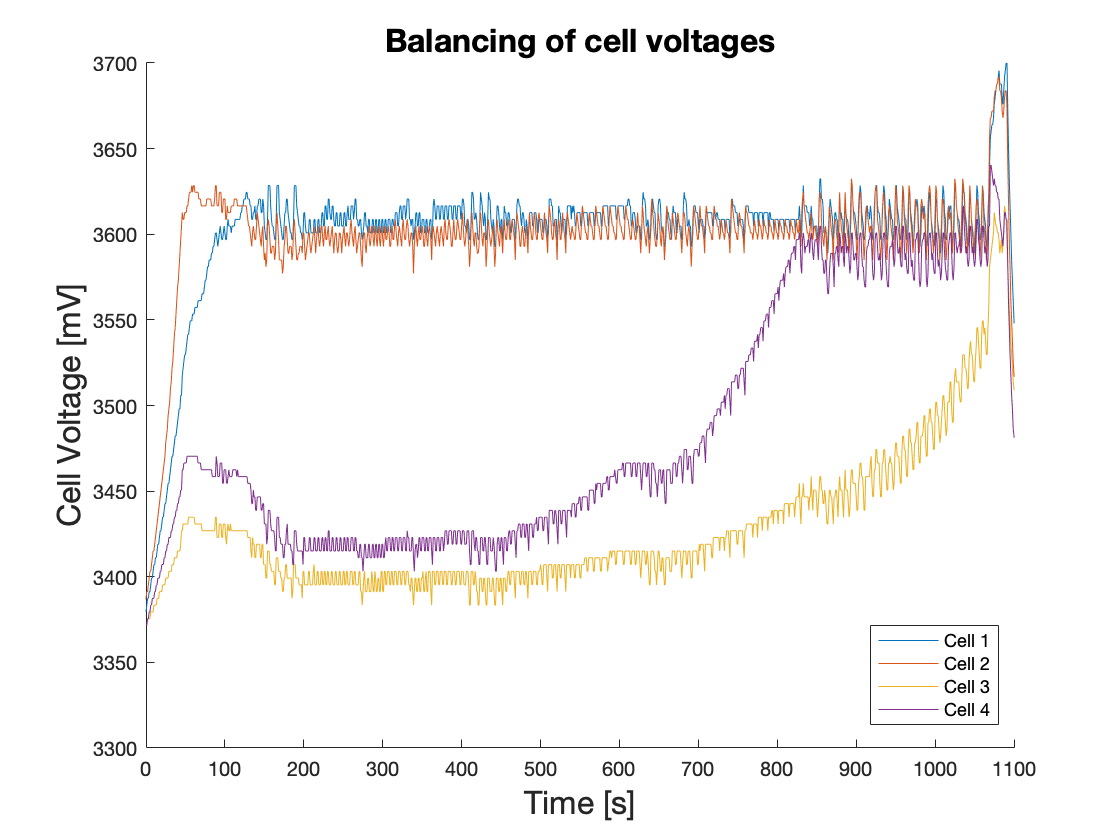
\includegraphics[width=\textwidth]{balancing.png}
      \caption{Cell voltages as they are being balanced, ignore voltage spikes at the end as they are not related to the balancing.}
      \label{fig:balancing}
    \end{minipage}
\end{figure}

\paragraph*{MPPT}
As previously discussed, the PV array should be operated in the region 
where the current is lower than at the maximum power point. To ensure 
this, the following algorithm was used. First, the duty cycle was set 
to 0. This makes the input impedance of the SMPS very high, leading 
to a near 0 PV array current. The duty cycle is then increased until 
the output current/voltage reaches its desired value. If the desired 
operating point requires less power than what the PV array can provide, 
then an equilibrium should be found as the duty cycle is increased. 
If however the desired operating point requires more power than the 
PV panels can provide, then no equilibrium can exist and the duty 
cycle will increase to 1 without ever reaching the desired operating 
point. Thus, if the duty cycle ever reaches 1 during operation the 
charging algorithm must be trying to draw more power from the PV 
array than is available. Whenever the duty cycle reaches 1, the 
variable \emph{max\_power}, is reduced by 100 mW and a new current 
setpoint is found through the 
formula $i_{setpoint} = max\_power / V_{out}$. The duty cycle 
is then reset to 0 and the process repeats until an equilibrium 
is found. When at an equilibrium, the algorithm increases 
\emph{max\_power} every 60 seconds to see if it is possible to 
operate at a higher power point than it currently is. If not, 
the algorithm will simply fall back to the same equilibrium. This 
algorithm was found to be very successful at tracking the maximum 
power point of the PV array. It is shown in action in the demo video.

\paragraph*{SOC}
\begin{wrapfigure}[13]{r}[0pt]{0.45\textwidth}
    \centering
    \raisebox{0pt}[\dimexpr\height-3\baselineskip\relax]{%
        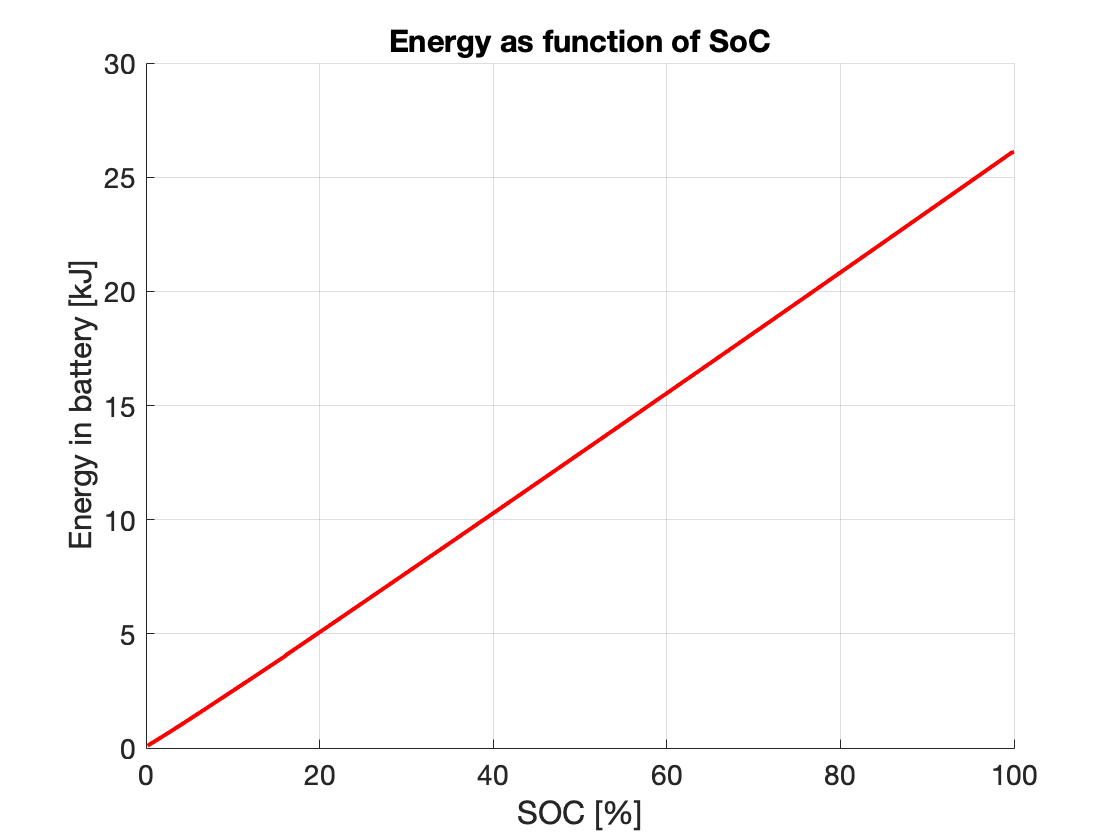
\includegraphics[width=0.45\textwidth]{lookup.png}
    }%
    \vspace{-10pt}
    \caption{Lookup table data}
    \label{fig:lookup}
\end{wrapfigure}

Implementing the Coulomb counting was done by integrating the current 
flowing into the battery. The integral value gives how much current 
has flowed in or out of the battery. The SOC as a percentage can 
then be found by dividing the net charge into the battery by the charge 
capacity of the battery and then multiplying by 100. However, due to
effects such as the Coulombic efficiency of the battery, the 
integral can start to stray when done over many cycles. As such, 
the SOC is reset to the maximum capacity every time the battery is 
fully charged. The maximum capacity will of course reduce over 
time as the battery degrades. This is why the maximum capacity is 
measured and updated with every discharge cycle. Moreover, as the 
Arduino is sometimes switched off before a charging/discharging 
cycle is complete, it is necessary to know the SOC on startup. 
As such, the current SOC is continually logged to the SD card during 
operation. When the Arduino is then switched on again, it simply 
fetches the SOC data from the SD card and continues at the SOC at 
which it left off. 

The SOC should be used to estimate the range of the rover. The 
obvious way of estimating the range is to divide the remaining energy 
in battery by the power consumption of the rover and multiply by 
the speed. However, the SOC does not directly give how much energy 
is in the batteries at any given time. To find the energy in the 
battery, the total expended energy was logged alongside SOC data 
for a full discharge of the battery. From this data a 600 element 
lookup table was created which related the SOC of the battery to 
the remaining energy in the battery. The lookup table data is plotted 
in Figure~\ref{fig:lookup}.

\paragraph*{Discharging}
The energy module is also tasked with keeping track of the SOC and SOH 
during discharging. This was done using the same algorithms as 
during charging. In addition the battery power was continually 
tracked as a function of time and SOC. When the battery is done d
ischarging, this information is used to update the table relating the 
SOC of the battery to the remaining usable energy. This is done using 
the formula 
\( New~Energy~Array = 0.99*(Old~Energy~Array) + 0.01*(Measured~Energy~Array) \). 
By having the energy array update itself it is hoped that the energy 
array will be a good approximation even after many battery cycles 
as the battery performance starts to deteriorate.

\paragraph*{Communicating with Other Modules}
Though it is not necessary to fully integrate the energy module with 
the rest of the rover, other submodules, specifically command, needs 
access data such as the battery SOH, SOC and remaining energy. For 
communicating with other modules the Arduino shield has a set of 
UART ports. However, as group members were not in the same location 
it was not possible to physically connect the energy module to the 
rover, which is necessary to use UART. As such, an alternative 
approach was employed. First the Arduino was connected to a computer 
via USB. On the computer a Python script was run. At the start, the 
Python script establishes a connection to a server created by running 
a similar script on the command module. After a connection has been 
established the Python script starts reading the serial data coming 
from the Arduino and transmits it using TCP to the command module. 
Each message coming from the Arduino is in CSV form where the first 
entry is the message ID, which allows the command script to decode 
what type of data is being sent. 
%End of energy implementation
%End of implementation section

\section{Evaluation and Conclusion}
\subsection{Testing}


    When testing the image processing and the Vision module, the camera had to 
    be recalibrated to match the testing enviroment. Initially, the only configurable
    parameters were the HSV thresholds as described in section 4.4.3, the exposure and
    the gain settings. This resulted in unsatisfactory performance as the testing enviroment
    was tinted yellow and there was no way of adjusting for that. 

    After researching the camera, and going through the OV8865's datasheet, \cite{OV8865DataSheet} it was discovered
    that white balance - the gains of the Red, Green and Blue pixels could be individual manipulated
    and manually calibrated. By testing these values with trial and error in conjunction with the 
    MATLAB Colour Threshold Tool, a set of gains were found that maximised the colour detection and
    reduced the number of false positives in the bounding box detection. This fixed the problem that 
    had occurred due to the tint of the room. 

    It was also noted in 
    initial testing that the corners of the camera were darker and dimmer than the rest 
    of the image, leading to difficulties in detecting objects that were in the corner
    of the frame due to different HSV values. This is a commonly seen phenomenon known as vignetting
    Although to the human eye, this may seem
    like a minor problem, for a computer vision algorithm, it can have highly detrimental 
    effects. \cite{zheng2008single} While also looking through the camera datasheet, 
    we realised that the OV8865 had a built in lens correction function that was not initially
    used. The lens correction algorithm on the OV8665 compensates for the vignetting effect by 
    calculating a gain for each pixel and correcting each pixel to compensate for the illumination
    drop off. \cite{OV8865DataSheet} By turning this on and using the default settings, 
    the problem was reduced and there was better illumination and colour pickup in the corners
    of the frame. Due to time constraints, the algorithm was not manually tuned to achieve
    the best results. 


\begin{comment}
    Could write about how we had to tune data for different lighting conditions, 
    taking pictures from different angles to compare how the objects looked in 
    different lighting, and changing the threshold values. 
\end{comment}

\section{Project Management and Organisation}
%Also had frequent teams meetings and used WhatsApp
As this project was carried out remotely
with contributors located in different countries, 
it was important to have a good framework for communication and management. 
For direct communications between the team, WhatsApp was used for short texts, 
and Microsoft Teams was utilised for calls as its screen-sharing functionality 
was useful for helping to debug errors. 

The main tool used for written communications and management was Git + GitHub.
As the codebase was incredibly complex, 
involving many different libraries and with each submodule being capable as a
standalone project, it was vital to have a version control system in place. 
Being able to keep a history of commits and changes made to a project was useful,
especially when trying to track down the origin of a bug and what caused it. 

The team also made use of GitHub Issues to track progress and accountability in 
the initial design phase. A thread was opened for each submodule to show what 
the lead for that submodule had been doing and potential avenues of achieving 
their goals. This was beneficial both for the leads to keep track of their 
research, but also allowed other members to contribute to other submodules 
by adding comments and voicing their thoughts. GitHub Issues were also linked 
directly to commits in the codebase to allow for a more in-depth explanation and
reasoning with context for a commit than what is allowed in the commit message 
area. 

By way of using GitHub, the team also made use of GitHub's Actions, which allow 
for automated workflows to be run on certain events like a commit or a push for 
continuous integration. An Action was designed for the writing of this report
that compiled the \LaTeX document and produced a PDF. 

Simultaneously, a Gantt chart was maintained to keep track of progress and is 
available for viewing under the maintained GitHub repository linked in the Appendix.

%TODO #7!
\section{Intellectual Property}
Intellectual Property (IP) is a complex topic that has financial, technological, 
and moral significance when developing products or inventions. In short, IP rights are what
lets companies, inventors and creators prevent other people from using their work\cite{perea}.
Many types of IP rights exists including copyrights, trademarks, design rights and patents.  

In the context of our design project, there are sections within IP which are less applicable than others. 
These include trademarks, as no brand is being developed, and design rights, as the rover's physical design has
been provided by the college and will not be significantly altered by students. Note however,
that as the college has created the rover design, it owns the design rights and could stop students
from using its appearance if desired, but would probably fail to obtain legal orders for it as the design
has been "publicly" circulated and freely provided.
Patenting is a vital step which should be encouraged for inventors to apply their negative rights and 
protect themselves from any infringement which seeks to use their original inventive work without permission. 
There are clear guidelines in place to determine what constitutes a patent and unfortunately, 
this is not the case for our rover. By no means is it a novel idea; all the technology being 
applied to the rover, like the hardware, communication protocols, vision algorithms and functionality 
have all been explored in depth and this could not be clearer when we look at the countless missions, 
development and papers that have been written for true Mars Rovers like Perseverance. 
Although there is a case to be made for industrial applicability, this first requirement being 
violated immediately nullifies the possibility of a patent. What is relevant is copyright as 
the combination of software algorithms being applied could be considered complex enough to assert 
copyright as it is original expression. However, as the Arduino and its libraries are under the GNU General 
Public License \cite{ArduinoLicense}, an open-source license, users need to follow the same license 
when using these libraries and we would hence be restricted to an (L)GPL license as well. A more complex 
situation is the system that is running on the FPGA, although all components are available for testing 
in what is known as the Intel FPGA IP Evaluation Mode, any commerical use of the IP would require a   
license to be bought from Intel\cite{IntelEvalMode}. There are few individual modules written in SystemVerilog that could be copyrighted, 
like the Image processing module and the image transfer over SPI module, if the FIFO and divider components were replaced
with either open-source/self-designed modules. 

\begin{comment}
This is just a draft, feel free to edit, add, remove, and change what you want.
Currently at 264 words
\end{comment}
\begin{comment}
Could link stuff about how we are using Intel IP in the FPGA, as well as things
like licencing and how some companies make their entire business based on it,
like Arm, hence ethically it is important to maintain standards and rules for IP
through the use of legislation and governmental regulatory authorities. 
\end{comment}
\begin{comment}
A lot of the technologies that we have used in this project is probably covered
by a patent.
\end{comment}
\begin{comment}
Could also talk about how some of the Libraries for the Arduino are open source
and the benefits that those bring to development in projects like these which
are not funded and the benefits of open source in general maybe?
\end{comment}

 
\newpage

\printbibliography[
heading=bibintoc,
title={References}
]


\newpage
\begin{appendices}


%\chapter{Appendix 1: Circuit Diagram of the Energy Submodule}
%\begin{figure}[H]
%    \centering
%    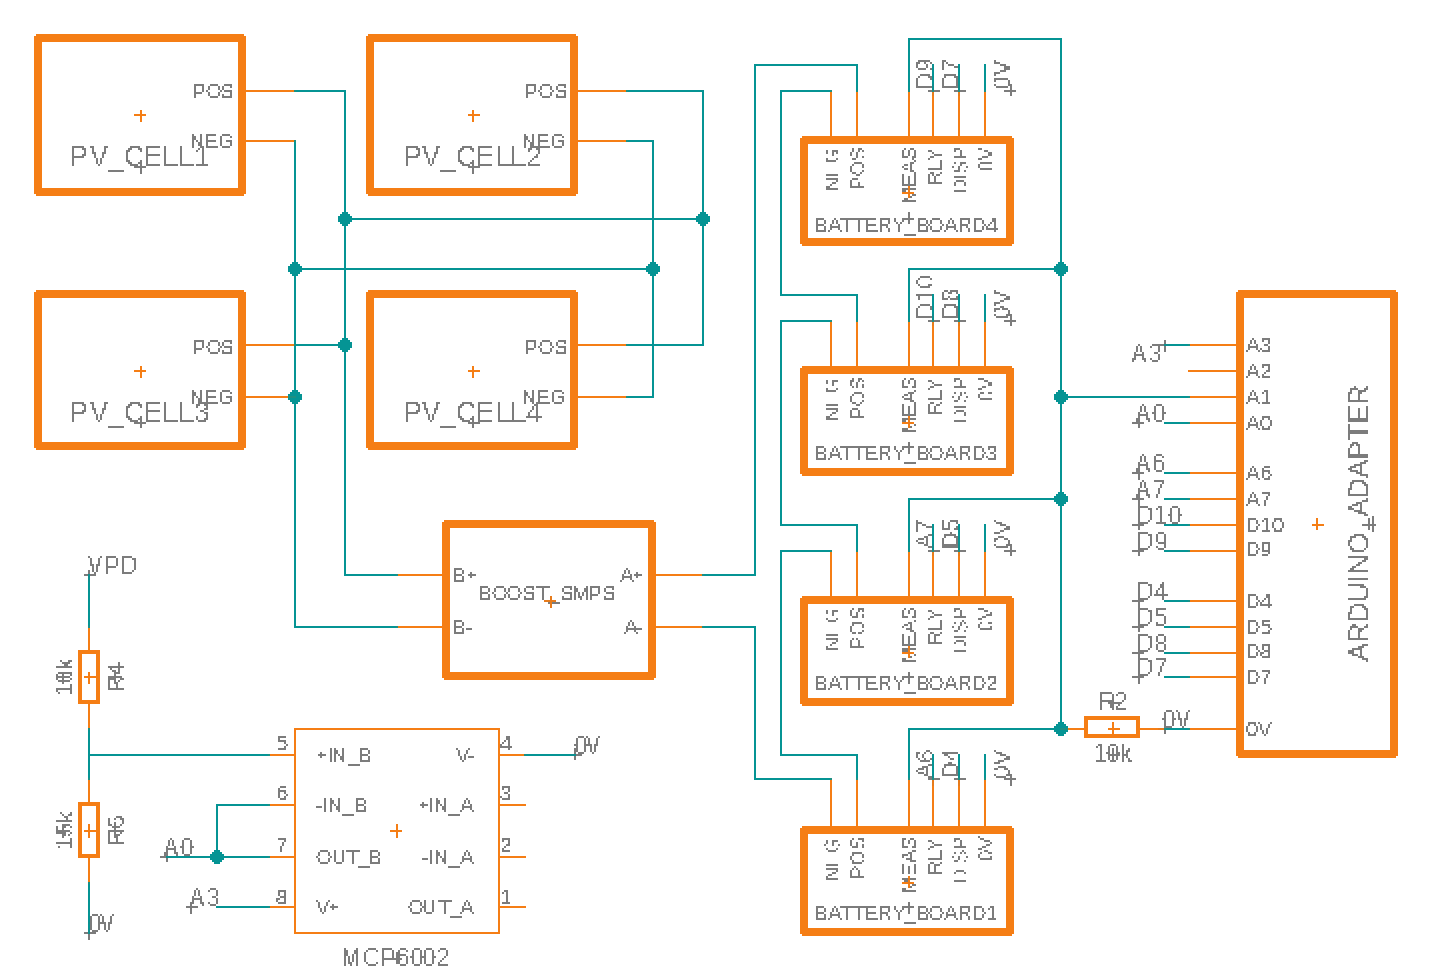
\includegraphics[width=\textwidth]{Circuit_Diagram.png}
%    \label{fig:circuitDiagram2}
%\end{figure}


\end{appendices}

\end{document}